\documentclass[openany,11pt,vi,oneside]{mitthesis}
\usepackage{lgrind}
\usepackage{calc}
\usepackage{cmap}
\usepackage{mathtools}
\usepackage{amssymb}
\usepackage{bm}
\usepackage{upgreek}
\usepackage{enumitem}
\usepackage{scrextend}
\usepackage{lscape}
\usepackage{geometry}
\usepackage{multicol}
\usepackage{multirow}
\usepackage{xcolor}
\usepackage{float}
\usepackage{afterpage}
\usepackage{rotating}
\usepackage{tabu}
\usepackage{booktabs}
\usepackage{graphicx}
\usepackage{subcaption}
\usepackage{nameref}
\usepackage{tikz}
\usepackage{matlab-prettifier}
\usepackage{listings}
\usepackage{mdframed}
\usepackage{minitoc-hyper}
%\usepackage[T1]{fontenc}
\usepackage[export]{adjustbox}
\usepackage[hang, flushmargin]{footmisc}
\usepackage[colorlinks,
            pdfusetitle]%
            {hyperref}
\usepackage[backend=biber,
            style=numeric,
            maxcitenames=2,
            sorting=none,
            url=false,
            isbn=false,
            doi=true,
            eprint=false]%
            {biblatex}
\hypersetup{citecolor={purple},linkcolor={blue}}
\usetikzlibrary{shapes,arrows.meta,calc}
%%%%%%%%%%%%%%%%%%%%%%%%%%%%%%%%%%%%%%%%%%%%%%%%%%%%%%%%%%%%%%%%%%%%%%%%%%%%%%%%%%%%%%%%%%%%%%%%%%%%
% resources
\addbibresource{./library.bib}
\graphicspath{{figs/}{figs/tikz/}{figs/tikz/algorithm/}{figs/ystd/}{figs/toy/}{figs/seg/}}
\newcommand{\matlabdir}{m/}
\makeatletter\newcommand{\setmaxcitenames}[1]{\numdef\blx@maxcitenames{#1}}\makeatother
\newcounter{papercount}
\newcommand{\citefortable}[1]{%
  \stepcounter{papercount}{\thepapercount}&{\cite{#1}}&{\citeyear{#1}}&{\citeauthor{#1}}}
% layout
\geometry{margin=2cm}
\setlength{\parindent}{0pt}
\setlength{\parskip}{8pt}
\setlength{\skip\footins}{24pt}
\setlength{\footnotemargin}{0.8em}
\renewcommand{\floatpagefraction}{.8}
\renewcommand{\textfraction}{.2}
%%%%%%%%%%%%%%%%%%%%%%%%%%%%%%%%%%%%%%%%%%%%%%%%%%%%%%%%%%%%%%%%%%%%%%%%%%%%%%%%%%%%%%%%%%%%%%%%%%%%
% math shorthands
\renewcommand{\Re}{\mathbb{R}}
\newcommand{\xxx}{\mathrm{x}_1,\mathrm{x}_2,\mathrm{x}_3}
\newcommand{\gm}{\textsc{gm}}
\newcommand{\wm}{\textsc{wm}}
\newcommand{\csf}{\textsc{csf}}
\newcommand{\wmh}{\textsc{wmh}}
\newcommand{\mrf}{\textsc{mrf}}
\newcommand{\lr}{\textsc{lr}}
\newcommand{\sk}{\textsc{k}}
\newcommand{\sn}{\textsc{n}}
\newcommand{\sr}{\textsc{r}}
\newcommand{\sv}{\textsc{v}}
\newcommand{\sx}{\textsc{x}}
\newcommand{\sy}{\textsc{y}}
\renewcommand{\d}{\partial}
\renewcommand{\b}{\beta}
\newcommand{\bb}{\bm{\beta}}
\newcommand{\by}{\bm{y}}
\renewcommand{\L}{\mathcal{L}}
\renewcommand{\P}{\mathcal{P}}
\newcommand{\N}{\mathcal{N}}
\newcommand{\J}{\mathcal{J}}
\newcommand{\Z}{\mathcal{Z}}
\newcommand{\Y}{\mathcal{Y}}
\newcommand{\C}{\mathcal{C}}
\newcommand{\X}{\mathcal{X}}
\newcommand{\bY}{\bm{\mathcal{Y}}}
\newcommand{\bC}{\bm{\mathcal{C}}}
\newcommand{\bV}{\bm{\mathcal{V}}}
\newcommand{\ep}{\circ}
\newcommand{\true}{\texttt{true}}
\newcommand{\false}{\texttt{false}}
\newcommand{\abs}[1]{\left|#1\right|}
\newcommand{\norm}[1]{\left|\left|#1\right|\right|}
\newcommand{\vox}[1]{\mathbb{#1}}
% scanner stuff
\newcommand{\sname}[1]{%
  \IfStrEqCase{#1}{%
    {01}{WMH 2017 (1)}
    {02}{WMH 2017 (2)}
    {03}{WMH 2017 (3)}
    {04}{MS  2016 (1)}
    {05}{MS  2016 (2)}
    {06}{MS  2016 (3)}
    {07}{ISBI MS 2015}
    {08}{In-House}
    {09}{MS  2008 CHB}
    {10}{MS  2008 UNC}
    {11}{T1 e.g.}
    {12}{T2 e.g.}}
  []}
\newcommand{\sclr}[1]{%
  \IfStrEqCase{#1}{%
    {00}{\color[rgb]{1.00 1.00 1.00}}
    {01}{\color[rgb]{1.00 0.00 0.00}}
    {02}{\color[rgb]{1.00 0.50 0.00}}
    {03}{\color[rgb]{1.00 0.80 0.00}}
    {04}{\color[rgb]{0.02 0.80 0.00}}
    {05}{\color[rgb]{0.00 0.40 1.00}}
    {06}{\color[rgb]{0.60 0.00 1.00}}
    {07}{\color[rgb]{1.00 0.00 1.00}}
    {08}{\color[rgb]{1.00 0.50 0.50}}
    {09}{\color[rgb]{0.50 1.00 0.70}}
    {10}{\color[rgb]{0.50 0.70 1.00}}}
  []}
\definecolor{gry}{rgb}{0.50 0.50 0.50}
\definecolor{blue}{rgb}{0.00 0.30 1.00}
% little text items
\renewcommand{\_}{\char`_}
\renewcommand{\ss}[1]{\textsuperscript{#1}}
\newcommand{\hreftt}[1]{\href{#1}{\footnotesize{\texttt{\lstinline|#1|}}}}
\newcommand{\et}{\thinspace}
\newcommand{\en}{\enspace}
\renewcommand\labelitemi{\raisebox{0.2em}{\fontsize{0.3em}{0}$\blacksquare$}}
\renewcommand\labelitemii{\raisebox{0.2em}{\fontsize{0.3em}{0}$\square$}}
\newcommand{\medfilt}[1]{\mathrm{Med}_{#1\times#1}}
\newcommand{\tablepost}[1]{\\[0.5em]\raggedright{\footnotesize{#1}}}
\newcommand{\subfigureoverl}[4][black]{%
  \begin{subfigure}{\textwidth}%
    \centering\setbox1=\hbox{#4}\leavevmode\rlap{\usebox1}%
    \rlap{\hspace*{0.5em}\raisebox{\dimexpr0.5em}{\color{#1}#2}}
    \phantom{\usebox1}\phantomsubcaption#3%
  \end{subfigure}}
% LaTeX penalties
\interfootnotelinepenalty=10000
\widowpenalty=500
\clubpenalty=500
% sizing
\newlength{\plotwidth}\setlength{\plotwidth}{0.48\textwidth}
\newlength{\sliceheight}\setlength{\sliceheight}{3.5cm}
\newlength{\fullheight}\setlength{\fullheight}{5cm}
\renewcommand*{\bibfont}{\footnotesize}
% appendix
\newcommand{\matlabsty}{\color{black}\ttfamily\footnotesize}
\global\mdfdefinestyle{graybar}{topline=false,rightline=false,bottomline=false,linewidth=0.2em,linecolor=lightgray,innertopmargin=0pt,innerbottommargin=0pt}
\lstnewenvironment{matlab}{%
  \linespread{1}\mdframed[style=graybar]%
  \lstset{style=Matlab-editor,basicstyle=\matlabsty,basewidth=0.5em}}%
  {\endmdframed}
\newcommand{\includecode}[1]%
  {\subsubsection[\ttfamily{#1}]{\hspace*{-1.5em}\ttfamily{>> #1}}\label{m:#1}%
  \begin{mdframed}[style=graybar]%
    \lstinputlisting[style=Matlab-editor,basicstyle=\linespread{1}\matlabsty]{\matlabdir#1}%
  \end{mdframed}}
%%%%%%%%%%%%%%%%%%%%%%%%%%%%%%%%%%%%%%%%%%%%%%%%%%%%%%%%%%%%%%%%%%%%%%%%%%%%%%%%%%%%%%%%%%%%%%%%%%%%
\begin{document}
  \title{Voxel-Wise Image Analysis\\for White Matter Hyperintensity Segmentation}
\author{Jesse Knight}
\department{School of Engineering}
\degree{Master of Applied Science}
\program{Engineering Systems and Computing}
\degreemonth{December}
\degreeyear{2017}
\thesisdate{2017-12-18}
\maketitle
\cleardoublepage{}
\pagenumbering{Roman}
\setcounter{page}{1}
\begin{abstractpage}
  White matter hyperintensities (WMH) are regions of increased pixel intensity
in T2-weighted magnetic resonance images (MRI)
which are correlated with several neurodegenerative diseases,
including vascular dementia and multiple sclerosis.
Manual segmentation of WMH -- labelling of image voxels as ``healthy'' or ``lesion'' --
is used for diagnosis and monitoring of these diseases.
However, human performance of this task is time consuming,
and is subject to variability which eclipses the subtle lesion changes of interest.
Therefore, automation of WMH segmentation is an attractive goal.
\par
While many algorithms for this task have previously been proposed
these have been generally either interpretable, or accurate, but not both.
Additionally, variability in protocols for estimating algorithm performance
has precluded robust identification of superior approaches.
In particular, few algorithms have been validated on MRI from different sources.
This is significant, since algorithms are often sensitive to
source-specific image features, including
inter-tissue contrasts, image resolution, scanner model, and field strength.
\par
This thesis addresses these two challenges.
First, a segmentation algorithm called
``Voxel-Wise Logistic Regression'' (VLR) is introduced,
which provides both good interpretability and good segmentation performance.
The model inspired by an existing open-source algorithm,
``Lesion Prediction Algorithm'' (LPA),
which uses fluid attenuation inversion recovery (FLAIR) MRI
to estimate the the WMH class probability image.
In the proposed VLR model,
all logistic regression feature weights are parameterized spatially
-- i.e.\ $\bm{\beta} \rightarrow \bm{\beta}(x)$ --
rather than just the intercept.
This significantly reduces training time and necessary modelling approximations,
and yields ``parameter images'' $\bm{\beta}(x)$
which concisely summarize the model class discrimination.
\par
Next, a validation framework called
``Leave-One-Source-Out Cross Validation'' (LOSO-CV) is introduced,
which provides more realistic estimation of model performance
on ``never-before-seen'' MRI sources.
Segmentation performance of the VLR model under LOSO-CV
is then used to guide optimization of pre- and post-processing operations,
as well as regularization strategies (incorporation of prior knowledge).
In the spirit of open research,
only data from recent WMH segmentation competitions
were used in this work, totalling 96 image sets from 7 MRI sources.
Additionally, the proposed algorithm will be deployed as a 3D Slicer application
for use by clinicians and researchers,
and source code for all investigations will be released on GitHub.

\end{abstractpage}
\cleardoublepage{}
\begin{titlepage}
  \begin{large}
    This masters thesis has been examined by \\ a Committee of the School of Engineering as follows:
    \signature{Hadis Karimipour}{Chair, Thesis Examination Committee \\
      Assistant Professor\\
      University of Guelph}
    \signature{April Khademi}{Thesis Co-Supervisor \\
      Assistant Professor\\
      Ryerson University}
    \signature{Graham Taylor}{Thesis Co-Supervisor \\
      Associate Professor\\
      University of Guelph}
    \signature{Medhat Moussa}{Member, Thesis Examination Committee \\
      Professor\\
      University of Guelph}
  \end{large}
\end{titlepage}
\section*{Acknowledgments}
I owe thanks to \dots
\\Jeremy, Danny, and Carly, for our cherished polemic forums;
\\Daniel, for sharing with me passions, pizza, and almost projects;
\\Thor, Colin, Terrance, and Dylan for our `deep' conversations;
\\Brayden, Aaron, and Carson, for board games and Jamaican bacon;
\\Erika, Denise, Emily, and Zyra, for bunting, crosswords, and Harambe;
\\My parents and Ali, for all your love and support;
\\and
\\My supervisors, for sharing with me your time, expertise, and so many opportunities.
\vfill
\begin{singlespace}
  \hspace*{4.0cm}\textit{If you want the truth to stand clear before you,}\\
  \hspace*{4.5cm}\textit{never be for or against.}                        \\
  \hspace*{4.0cm}\textit{The struggle between `for' and `against'}        \\
  \hspace*{4.5cm}\textit{is the mind's worst disease.}                    \\[0.5em]
  \hspace*{9.0cm}\normalfont{} --- Sent-ts'an c. 700 C.E.
\end{singlespace}

	%\pagenumbering{Roman}
\begin{singlespacing}
\tableofcontents
\newpage
\listoffigures
\newpage
\listoftables
\newpage
\subsection*{Abbreviations}
\begin{table}[H]
  \begin{tabular}{ll}
  	\hline
  	GM      & Grey matter                          \\
  	WM      & White matter                         \\
  	CSF     & Cerebrospinal fluid                  \\
  	PD      & Proton density                       \\
  	FLAIR   & Fluid attenuation inversion recovery \\
  	WML     & White matter lesion                  \\
  	WMH     & White matter hyperintensity          \\
  	DAWM    & Dirty appearing WM                   \\
  	MS      & Multiple Sclerosis                   \\
  	AD      & Alzheimer's Disease                  \\
  	PVE     & Partial volume effect                \\
  	VLR     & Voxel-Wise Logistic Regression       \\
  	MLE     & Maximum likelihood estimation        \\
  	MAP     & Maximum a posteriori                 \\
  	SI      & Similarity index                     \\
  	ICC     & Interclass Correlation Coefficient   \\
  	LL      & Lesion load                          \\
  	CV      & Cross validation                     \\
  	LOO-CV  & Leave-one-out CV                     \\
  	KF-CV   & K-fold CV                            \\
  	LOSO-CV & Leave-one-source-out                 \\
  	SVM     & Support vector machine               \\
  	K-NN    & K-nearest neighbours                 \\
  	MRF     & Markov random field                  \\
  	FPR     & False positive reduction             \\
    PMF     & Probability mass function            \\
    CDF     & Cumulative density function          \\ \hline
  \end{tabular}
\end{table}
\clearpage
\subsection*{Notation}
\begin{table}[H]
  \begin{tabular}{lll}
  	\hline
  	\multicolumn{3}{l}{Variables}                                                              \\ \hline
  	$y$                   & feature                                      & $\in\Re$            \\
  	$\tilde{y}$           & standardized feature                         & $\in\Re$            \\
  	$c$                   & true class                                   & $\in\{0,1\}$        \\
  	$\hat{c}$             & estimated class                              & $\in[0,1]$          \\
  	$\beta$               & logistic model feature weight                & $\in\Re$            \\
  	$\gamma$              & synthetic feature                            & $\in\Re$            \\
  	$\rho$                & prior probability                            & $\in[0,1]$          \\ \hline
  	\multicolumn{3}{l}{Indexing -- e.g. arbitrary variable $a$}                                \\ \hline
  	$k$                   & feature index                                & $\in \{1,\dots,K\}$ \\
  	$n$                   & subject index                                & $\in \{1,\dots,N\}$ \\
  	$t$                   & iteration index                              & $\in \{1,\dots,X\}$ \\
  	$x$                   & spatial location                             & $= [\xxx]$          \\
   	${a_n^k}^{(t)}(x)$    & $k$\ss{th} feature; $n$\ss{th} subject; $t$\ss{th} iteration; location $x$ & \\ \hline
  	\multicolumn{3}{l}{Images \& sets -- e.g. arbitrary variable $a$}                          \\ \hline
  	$a$                   & one voxel, one feature, one subject          &                     \\
  	$\bm{a}$              & one voxel, all features, one subject         &                     \\
  	$\mathrm{A}(x)$       & image in native space                        &                     \\
  	$A(x)$                & image in standard space (MNI)                &                     \\
  	$\bm{A}(x)$           & image set: all features, one subject         &                     \\
  	$\mathcal{A}(x)$      & image set: one feature, all subjects         &                     \\
  	$\bm{\mathcal{A}}(x)$ & image superset: all features, all subjects   &                     \\
  	$\vox{A}$             & full dataset: all features, subjects, voxels &                     \\ \hline
  \end{tabular}
\end{table}
\end{singlespacing}
\clearpage
\pagenumbering{arabic}
\setcounter{page}{1}

  %%%%%%%%%%%%%%%%%%%%%%%%%%%%%%%%%%%%%%%%%%%%%%%%%%%%%%%%%%%%%%%%%%%%%%%%%%%%%%%%%%%%%%%%%%%%%%%%%%%%
% ==================================================================================================
% --------------------------------------------------------------------------------------------------
\chapter{Introduction}
Digitization of medical imaging has facilitated innumerable advances in disease understanding and treatment. From multi-modal image fusion to image guided therapy, software tools now underpin research and clinical workflows in almost every domain of medical imaging.
\par
This work concerns an unsolved segmentation problem in 3D brain magnetic resonance imaging (MRI), in which the objective is to automatically predict the class, or label, of every voxel (``volume pixel'') in the image. The objects of interest are white matter hyperintensities (WMH), non-cancerous brain lesions which are correlated with several neurodegenerative diseases. This chapter presents the motivation for automated WMH segmentation, gives a problem definition, and explores the previously proposed solutions.
%%%%%%%%%%%%%%%%%%%%%%%%%%%%%%%%%%%%%%%%%%%%%%%%%%%%%%%%%%%%%%%%%%%%%%%%%%%%%%%%%%%%%%%%%%%%%%%%%%%%
\section{Background}
The brain is composed of three major classes of tissue: grey matter (GM), white matter (GM), and cerebrospinal fluid (CSF). Grey matter constitutes the peripheral surface of the brain -- the cortex, approximately 5mm thick -- as well as some deeper structures called the basal ganglia. It contains neuronal cell bodies, and performs the bulk of neural processing. The white matter is composed primarily of myelinated axons, and functions to relay information between different GM structures in the brain. The brain is surrounded by CSF, which provides mechanical and immunological defence. It is produced by the choroid plexuses in the ventricles of the brain -- a series of 4 connected cavities.
% ==================================================================================================
\subsection{Magnetic Resonance Imaging}\label{ss:mri}
Magnetic resonance imaging (MRI) provides superior and flexible brain tissue contrast versus computed tomography (CT) imaging, and is the primary modality for imaging brain disease. Whereas CT measures tissue density via attenuation of transmitted X-rays, which does not vary significantly among brain tissues, MRI measures a mutable combination of 3 tissue characteristics: the proton density (PD)\footnote{MRI can be used to image any nucleus with a net nuclear dipole, but proton (hydrogen) imaging is most common since hydrogen is biologically abundant and gives a strong signal intensity.}, and T1 and T2 relaxation constants \cite{Pooley2005}. The physics of signal generation are described below.
\par
\begin{figure}[b]
  \centering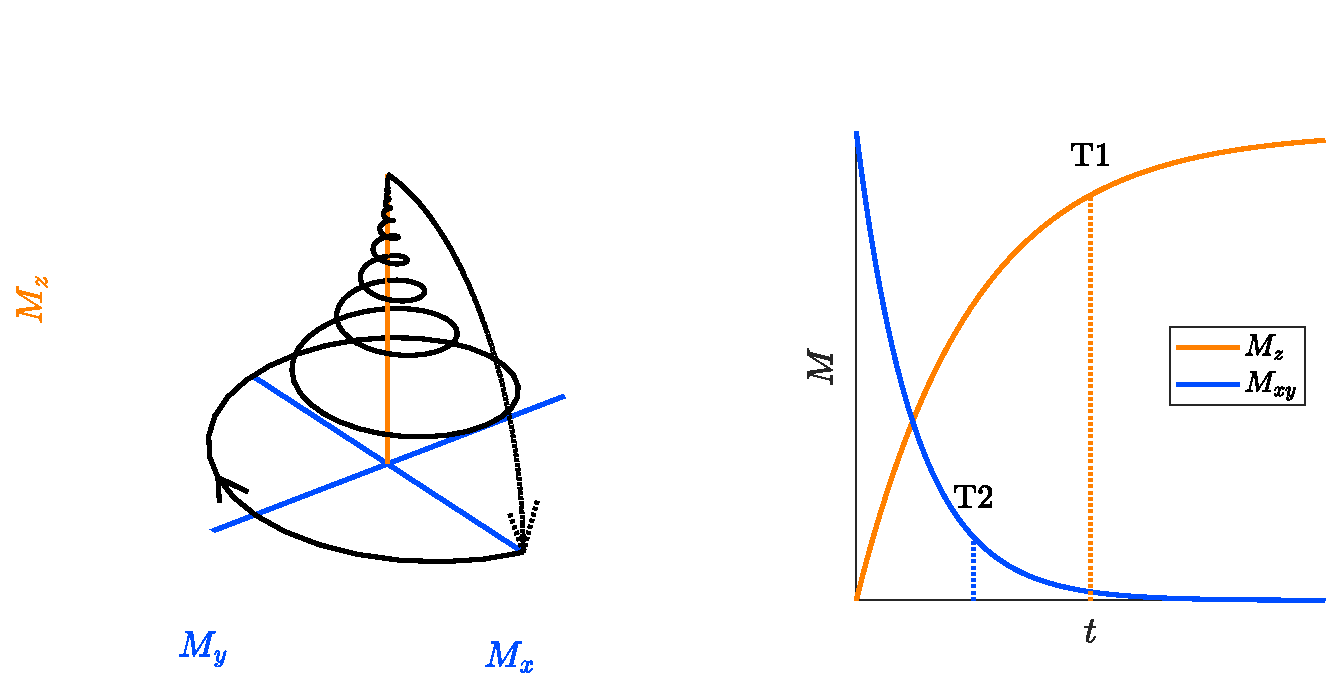
\includegraphics[width=\plotwidth]{mridecay3d}
  \caption{Visualization of T1 and T2 relaxation}
  \label{fig:mridecay3d}
\end{figure}
In an MR scanner, a powerful magnetic field induces alignment of proton dipoles with the field. Only a tiny fraction of the total protons align, but they create a small magnetic field $M_z$ which is distinct from the main field \cite{Bloch1946}. The aligned protons also rotate about the axis of alignment, imperfectly, like a spinning top; this is called precession, and the frequency of rotation is roughly homogeneous and proportional to the main field strength \cite{Bloch1946}. If a second magnetic field is applied which is $90^{\circ}$ perpendicular to the first, and rotating at the precession frequency, the aligned protons can be forced into temporary alignment with this transverse rotating field, before decaying back towards their original state, as illustrated in Figure \ref{fig:mridecay3d} \cite{Bloch1946}. This transient applied magnetic field is induced by a radio frequency (RF) pulse, and the rate at which the original magnetization $M_z$ is regained is described by the tissue-specific T1 relaxation constant,
\begin{equation}
M_z = M_0\et\left(1-e^{-\left(\frac{t}{T1}\right)}\right)\label{eq:T1}.
\end{equation}
The T1 constant is dictated by the ability of protons in the tissue to transfer energy to bonded atoms and surrounding molecules, since this energy transfer defines the transition from the high energy transverse state to the low energy original state \cite{Bloch1946,Bryant2005}. Large macromolecules, membranes, and lipids are generally able to facilitate this energy transfer more effectively than small molecules like water, producing a shorter T1 \cite{Koenig1990}. For this reason, myelinated WM has a shorter T1 than GM, which in turn has a shorter T1 than CSF, which is mostly water \cite{Roberts2007}.
\par
The rate of decay of the transverse moment $M_{xy}$ is actually not equal to the rate of regeneration of $M_z$. Rather, this is governed by the T2 relaxation constant,
\begin{equation}
M_{xy} = M_0\et\left(e^{-\left(\frac{t}{T2}\right)}\right)\label{eq:T2},
\end{equation}
which is always shorter that T1. This is because, in addition to T1 effects, the net rotating moment $M_{xy}$ is eroded by proton dephasing. When precessing protons, having a net dipole, interact with other dipoles or charged particles, their rotational frequency can be increased or decreased, but overall less coherent, reducing the perceptible net magnetization $M_{xy}$ \cite{Bloch1946}. In highly structured tissues like GM and WM, these interactions are more variable, dephasing is faster, and T2 is shorter \cite{Roberts2007}. In fluid environments like CSF, proton interactions are more homogeneous, yielding longer T2 \cite{Roberts2007}. For this reason, T2-weighted images are especially useful in identifying pathologies which degrade tissue structure, since they will have abnormally high T2 \cite{Roberts2007}. Both relaxation constants depend in a small way on the main magnetic field strength, measured in Tesla (T); T1 and T2 values for various brain tissues at 1.5T are summarized in Table \ref{tab:t1t2tissues}.
\par
\begin{table}
  \caption{T1 and T2 constants for brain tissues at 1.5 Tesla.}
  \label{tab:t1t2tissues}
  \centering{\setlength{\tabcolsep}{2pt}
    \begin{tabular}{ccrclcrclcrclcl}\hline
      Tissue && \multicolumn{3}{c}{T1 (ms)} && \multicolumn{3}{c}{T2 (ms)} && \multicolumn{3}{c}{$K [H]$ (a.u.)}&& Ref\\\hline
      WM  &&  719 & $\pm$ &  33 &&   73 & $\pm$ &   6 && 0.81 & $\pm$ & 0.03 && \cite{Schmitt2004}\\
      GM  && 1165 & $\pm$ &  88 &&   92 & $\pm$ &  11 && 0.98 & $\pm$ & 0.07 && \cite{Schmitt2004}\\
      CSF && 3337 & $\pm$ & 111 && 2562 & $\pm$ & 123 && 1.00 & $\pm$ & 0.07 && \cite{Schmitt2004}\\
      WML && 1124 & $\pm$ & 372 &&  136 & $\pm$ &  79 &&      &  $-$  &      && \cite{Stevenson2000}\ss{a}\\
      \hline
  \end{tabular}}
  \tablepost{\ss{a} Estimated from Fig 1 supratentorial data (numerical results not given); $\pm$ IQR, not SD; cf. \ref{ss:WMD} for definition.}
\end{table}
Image acquisition involves sensing the transverse magnetization $M_{xy}$ following proton excitation by an RF pulse. The problem is that this small signal decays very quickly due to proton dephasing, which occurs even faster than $T2$ would predict due to a third factor, inhomogeneity in the main magnetic field \cite{Chavhan2009}. The time constant for this decays is termed $T2^*$, and its effects are usually undesirable \cite{Chavhan2009}. As a result, $M_{xy}$ is easily overpowered by the magnetic moment from the RF pulse, even after it is turned off, due to resonance. An important solution to this, called the spin-echo, was proposed by Erwin Hahn in \citeyear{Hahn1950} \cite{Hahn1950}. If $T2^*$ for each proton is assumed to be constant, then reversing the direction of rotation at a time $t$ should cause all protons to align again at exactly $2t$. Therefore, at $2t$ the transverse magnetization $M_{xy}$ -- the image signal -- manifests again for sensing, no longer confounded by RF coil resonance \cite{Hahn1950}.
\par
This second signal is called the Spin Echo ($SE$), and the interval $2t$ is termed the echo time ($TE$). Reversing the direction of rotation can be achieved by a $180^{\circ}$ RF pulse at time $TE/2$, in the same way the original excitation is achieved using a $90^{\circ}$ RF pulse (amount of rotation is proportional to the energy of the pulse). Acquisition of an entire image requires repetitions of this sequence with an interval called the repetition time ($TR$). An example spin echo sequence, showing $TE$ and $TR$, as well as $T1$ and $T2$ decay, is illustrated in Figure \ref{fig:mrispinecho}. Spatial encoding for creation of 2D and 3D images requires the use of additional electromagnetic gradients; however this topic is omitted here since it is quite involved, and not essential to the current work\footnote{The interested reader is directed to this comprehensive resource on the topic: \hreftt{http://mri-q.com/}}.
\par
\begin{figure}
  \centering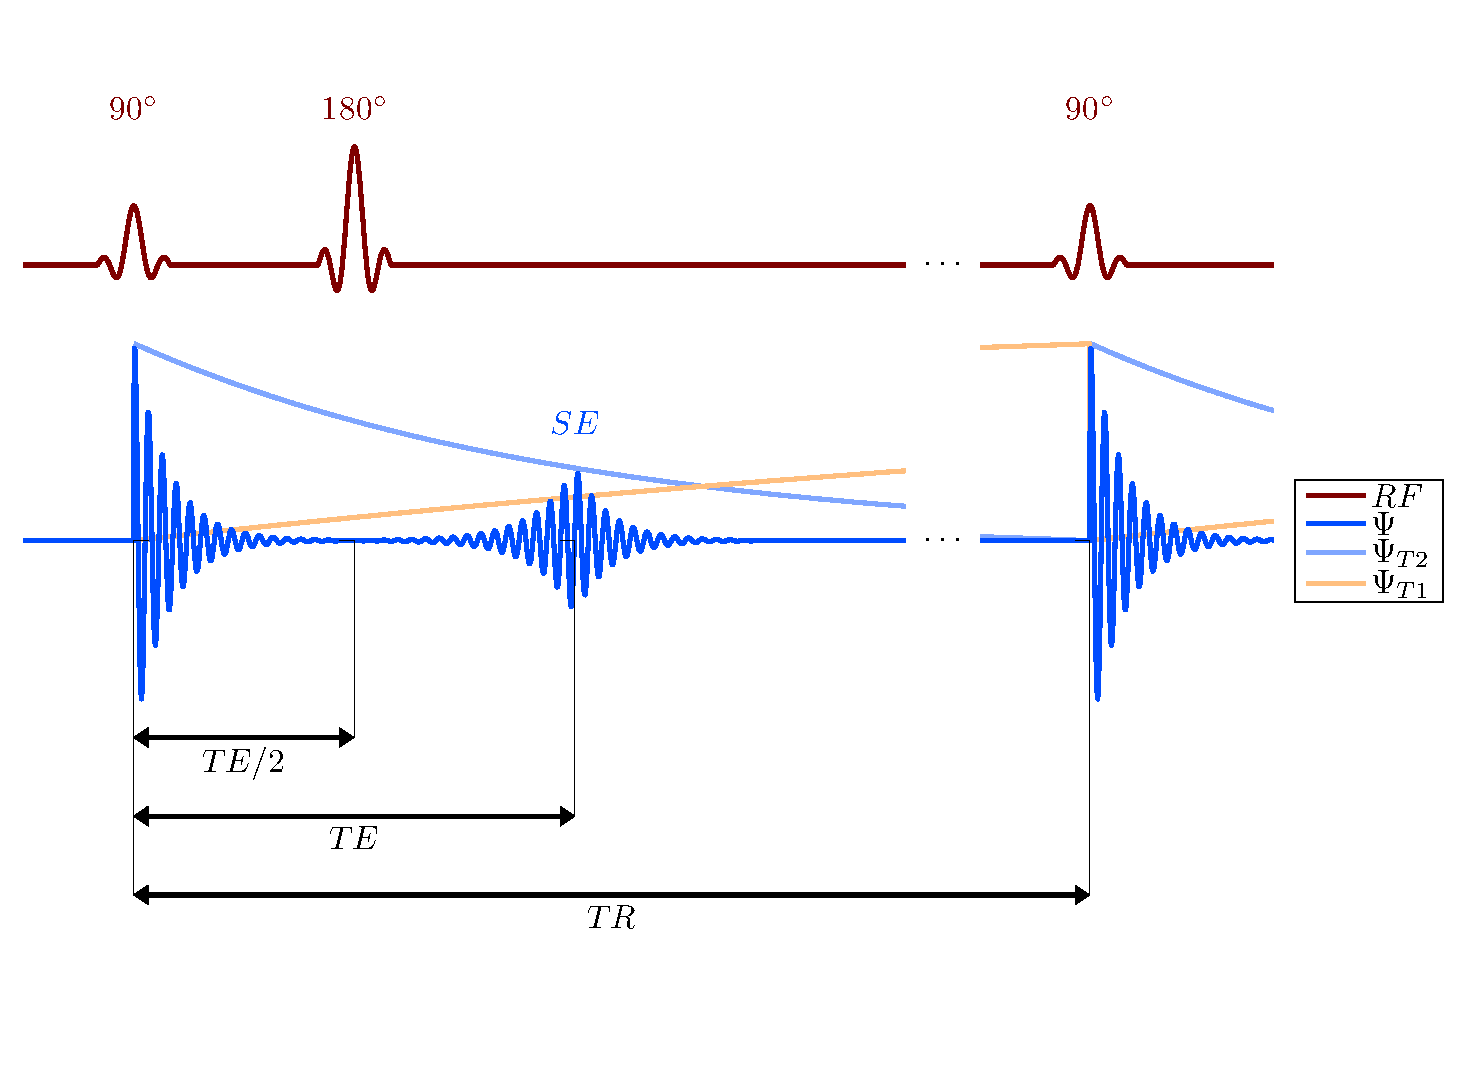
\includegraphics[width=\plotwidth]{mrispinecho}
  \caption{RF and MR signal for a basic Spin Echo sequence}
  \label{fig:mrispinecho}
\end{figure}
Using these principals, the nature of MR image contrast can finally be understood. That is, the signal intensity $\Psi$ for a spin echo sequence at location $x$ can be described by the following 3-term equation,
\begin{equation}\label{eq:MRI-SE}
\Psi_{SE}(x) = \bigg[K [H](x)\bigg]\bigg[e^{-\left(\frac{TE}{T2(x)}\right)}\bigg]\bigg[1 - e^{-\left(\frac{TR}{T1(x)}\right)}\bigg],
\end{equation}
where $K$ is scaling factor, and $\left[H\right]$ denotes the proton density. If $TR$ is chosen to be relatively long, then the longitudinal magnetization $M_z$ is allowed to recover completely after each repetition, the third term tends towards 1 for all tissues, and differences in tissue specific $T1$ are nullified. Similarly, if $TE$ is relatively short, then $M_{xy}$ has little time to dephase, the second term is maintained close to 1, and differences in $T2$ are nullified. In order to emphasize differences in $T1$, therefore, $TR$ can be chosen shorter; for $T2$-weighted contrast, $TE$ can be chosen longer; and if differences in $[H]$ (proton density, PD) are to be emphasized, $TR$ can be kept long and $TE$ short. An example MRI slice using each of these image sequences is shown in Figure \ref{fig:4mriT1}, \ref{fig:4mriT2}, and \ref{fig:4mriPD}.
\par
For identifying WML, T2-weighted images were conventionally used, since the lesions appear bright. However, CSF in the sulci and ventricles also appears bright on T2 images, making delineation of lesions -- especially periventricular ones -- difficult in T2 images (Figure \ref{fig:4mriT2}). To solve this problem, an adaptation of the spin echo RF pulse sequence can be used, called an inversion recovery (IR) \cite{Bydder1985}. In this sequence, an additional $180^{\circ}$ inverting RF pulse is added before the $90^{\circ}$ pulse, so that the longitudinal magnetization $M_z$ is inverted, then recovers to the original state, passing for a brief moment through zero net magnetization. The rate of recovery is governed by $T1$, so it is tissue specific. Furthermore, if the $90^{\circ}$ pulse is applied at the instant of zero net magnetization, no transverse moment will develop, nor the subsequent spin echo. Therefore this time interval, called the inversion time ($TI$), can be chosen to null the signal from any tissue with a unique $T1$. The equation governing the image signal simply adds an inversion term,
\begin{equation}\label{eq:MRI-IR}
\Psi_{IR}(x) = \bigg[K \left[H(x)\right]\bigg]\bigg[e^{-\left(\frac{TE}{T2(x)}\right)}\bigg]\bigg[1 + e^{-\left(\frac{TR}{T1(x)}\right)} - 2e^{-\left(\frac{TI}{T1(x)}\right)}\bigg].
\end{equation}
This inversion principal is now often used to null the signal from CSF, especially for delineation of WMH, in a sequence called FLuid Attenuation Inversion Recovery (FLAIR) \cite{Hajnal1992}. FLAIR images are usually T2-weighted. Figure \ref{fig:4mriIR} shows an example FLAIR image, where a WMH can be seen, posterior to the occipital horn of the left lateral ventricle, much more clearly than in the T2 image.
\begin{figure}
  \centering
  \begin{subfigure}{0.24\textwidth}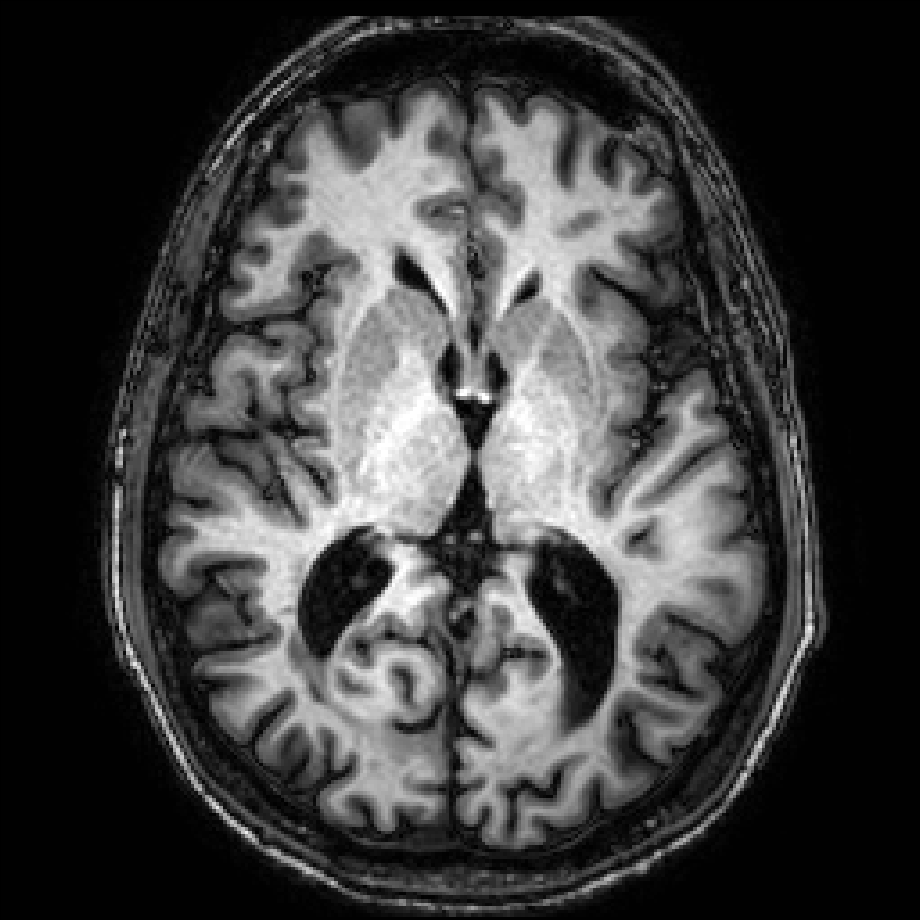
\includegraphics[width=\textwidth]{i15_training01_01_mprage.png}\caption{T1}  \label{fig:4mriT1}\end{subfigure}
  \begin{subfigure}{0.24\textwidth}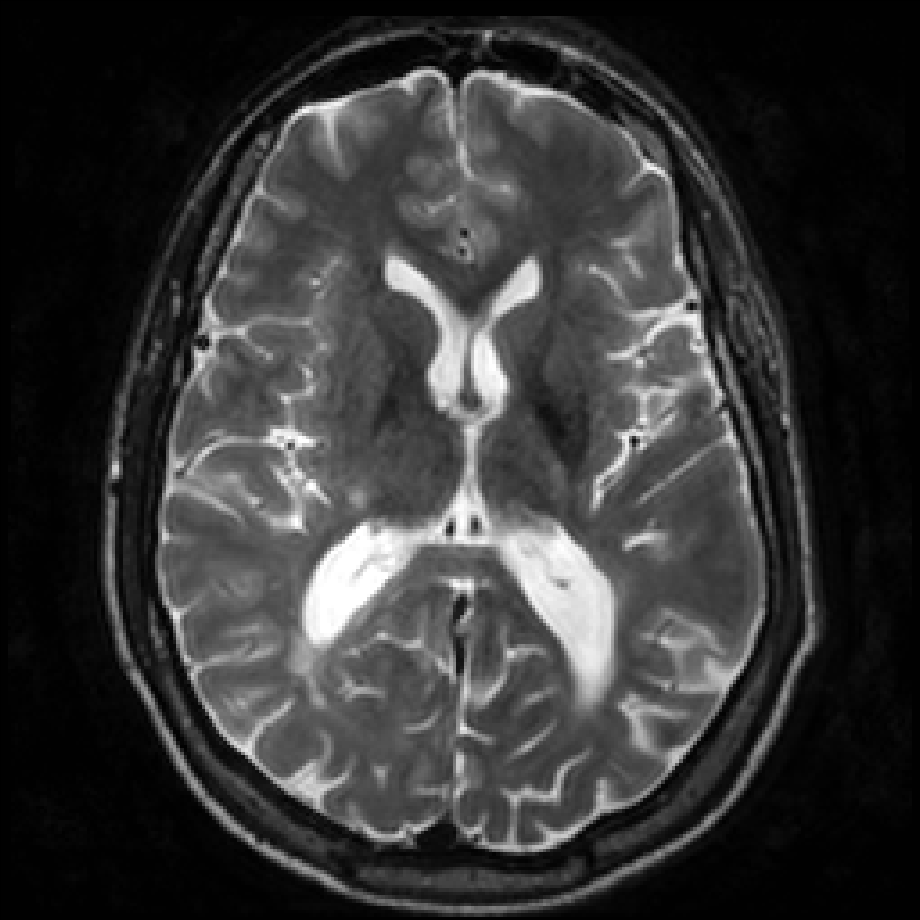
\includegraphics[width=\textwidth]{i15_training01_01_t2.png}\caption{T2}      \label{fig:4mriT2}\end{subfigure}
  \begin{subfigure}{0.24\textwidth}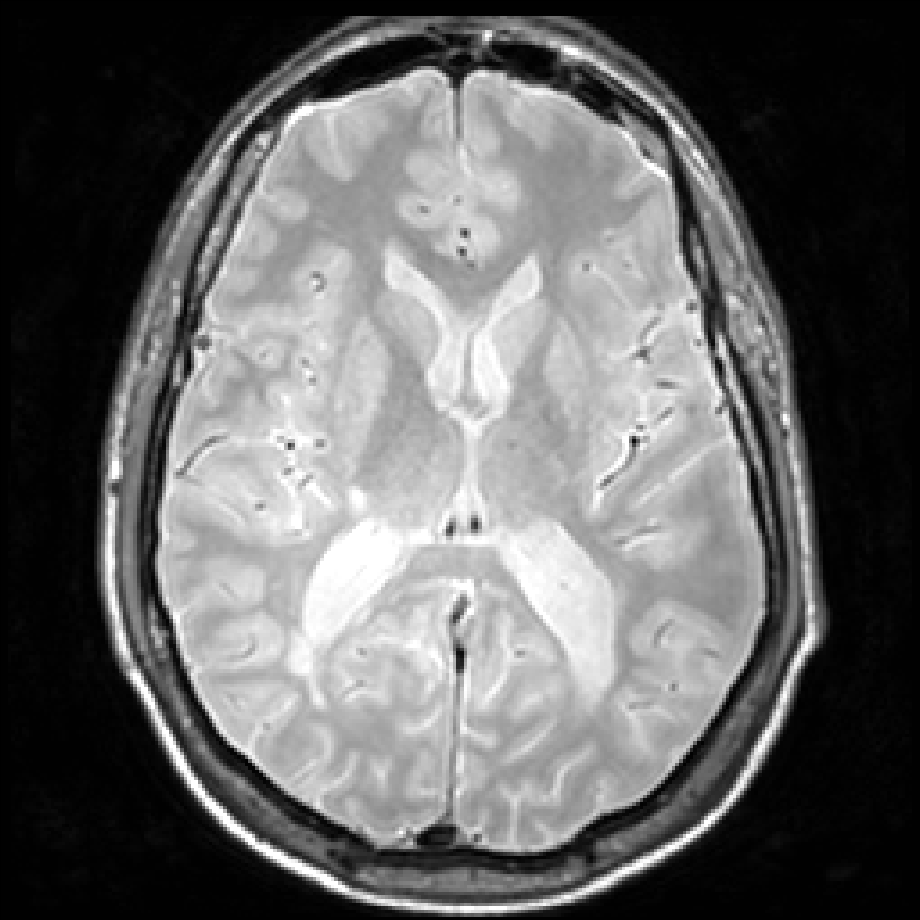
\includegraphics[width=\textwidth]{i15_training01_01_pd.png}\caption{PD}      \label{fig:4mriPD}\end{subfigure}
  \begin{subfigure}{0.24\textwidth}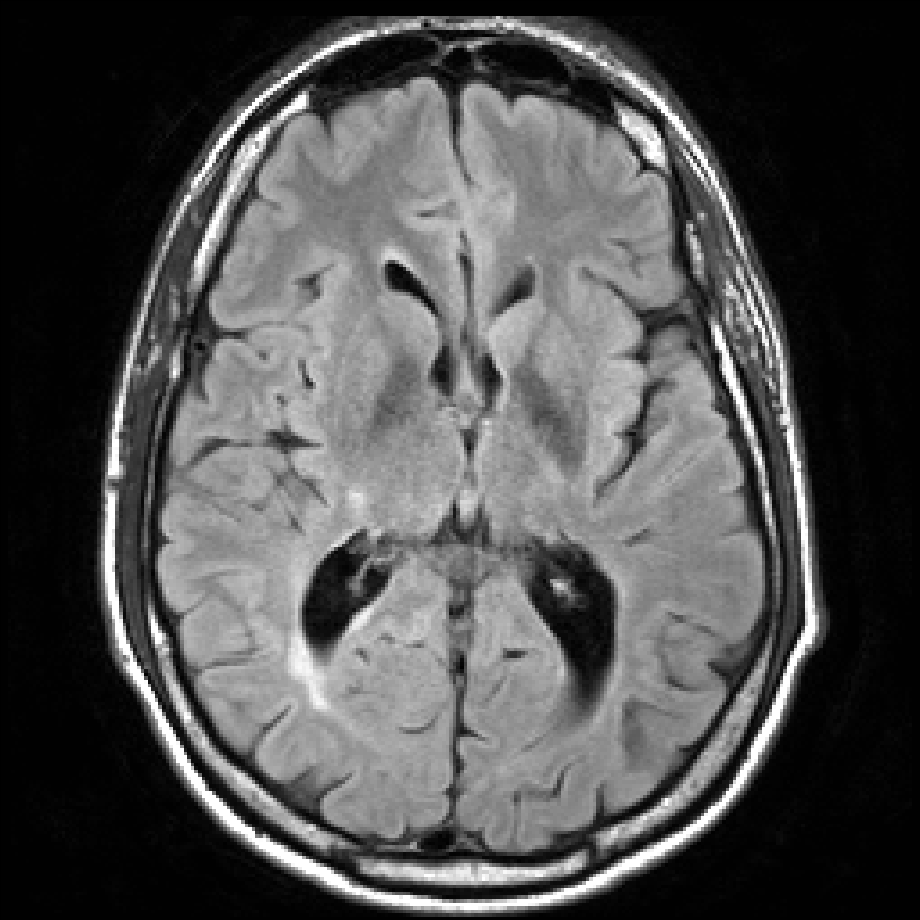
\includegraphics[width=\textwidth]{i15_training01_01_flair.png}\caption{FLAIR}\label{fig:4mriIR}\end{subfigure}
  \caption{Example MRI image set with WMH pathology; from \cite{WMHSEG2017}}
  \label{fig:4mri}
\end{figure}
% ==================================================================================================
\subsection{White Matter Disease}\label{ss:WMD}
``Normal'' ageing of the brain is characterized by a variety of physical and cognitive changes. Memory, synaptic plasticity, and brain volume decline, with observable effects on cognitive function \cite{Peters2006,Good2002}. Brain ageing is also expedited in many patients by neurodegenerative diseases targeting the white matter, including Alzheimer's disease (AD), cerebrovascular disease, and in rare cases Multiple Sclerosis (MS). While the etiologies of these diseases are not yet fully understood, there is considerable evidence to suggest that the they are intertwined \cite{Debette2010,Conklin2014,Heppner2015,Snyder2015}.
\par
Cerebrovascular disease describes changes to blood vessels in the brain which increase the risk of ischemic injury -- a reduction in blood flow due to vessel occlusion or hemorrhage. Ischemic injuries include major events (stroke) \cite{VanderWorp2007}, transient ischemic attacks \cite{Albers2002}, and chronic hypoperfusion due to small vessel disease \cite{Pantoni2010}. In all such events, neuronal death occurs from insufficient nutrient supply \cite{VanderWorp2007}. Strokes involving major cerebral arteries can be fatal, and post-event quality of life in survivors is highly variable \cite{Prabhakaran2015}. In the less dramatic courses, clinically quiet disease progression can lead to personality changes, memory loss, and reduced cognitive ability; such changes are termed vascular dementia \cite{Roman1993}.
\par
Alzheimer's Disease is another subclass of dementia with similar symptoms; in fact it is the most common type, affecting about 6\% of the population over age 65 \cite{Burns2009}. The cause of Alzheimer's disease is hotly debated. Two 30-year-old theories linking the disease to the build up of amyloid $\beta$ protein and misfolded protein $\tau$ have been widely supported by correlational studies \cite{Masters1985,Hardy2002,Lee2011}, but have lacked clear mechanisms of injury until recently. It is now thought that amyloid $\beta$ oligomers interfere with neuronal mitochondria and synapse function, leading to cell death \cite{Kim2013,Tu2014}, while aberrant $\tau$ proteins disrupt microtubules necessary for intraneuronal transport \cite{Lee2011}. During the search for these mechanisms, competing theories implicating vascular injury \cite{Snyder2015}, immune response \cite{Heppner2015}, and blood brain barrier disruption \cite{Bell2009} have emerged, painting the picture of a more complex disease.
\par
The pathophysiology of multiple sclerosis is similarly unclear, though genetics are a necessary factor, and it is known that symptoms arise from erosion of myelin -- a fatty insulating layer surrounding axons which is critical for normal neuron firing \cite{Trapp2008}. Several theories hypothesize either that this damage is driven by autoimmune attack, followed by neuronal dysfunction and death, or that neurodegenerative changes stimulate recruitment of immune cells as part of the usual response to injury \cite{Lucchinetti2000,Trapp2008}. Recent evidence favours the former mechanism, particularly with inflammatory injury as the initiating event \cite{Ciccarelli2014,Mahad2015}.
%A helpful visualization of MS lesion progression over one year is available here\footnote{\hreftt{http://www.msdiscovery.org/sites/default/files/MGrid\_crop4\_full\_0.gif}}.
\par
Connecting all these diseases are white matter lesions (WML, \textsc{aka} Leukoariosis), which represent the macroscopic changes to brain tissue in regions of white matter damage \cite{Debette2010,Bakshi2005,Wardlaw2015}. WML are very common in elderly populations, and a small volume of lesion does not necessarily implicate one of the above diseases; in one study of 1077 subjects aged 60-90, 95\% had at least one WML \cite{DeLeeuw2001}. WML appear as bright tissue regions in T2-weighted MRI due to some combination of inflammatory injury and degradation of tissue structure \cite{Bakshi2005,Wardlaw2015}; in this imaging context, they are often called white matter hyperintensities (WMH). Lesions are often focal, as opposed to diffuse, but there is evidence to suggest that surrounding regions of moderate hyperintensity, sometimes called ``dirty appearing white matter (DAWM)'', are also related to the diseases \cite{Ge2003}. As biomarkers of the most common WM diseases -- conditions with unsolved etiologies and inadequate treatments -- WML are of special interest to many brain researchers. The next section discusses how they are used.
% ==================================================================================================
\subsection{MRI in White Matter Disease}
MR imaging plays important roles in diagnosis and research of white matter diseases. Typical MRI protocols include T1, T2, and FLAIR sequences, though only the latter two sequences depict WML as hyperintense \cite{Simon2006,Wardlaw2013}. Depending on the disease and context, WMH can be quantified in several ways, including binary criteria (e.g. is there a lesion in a  specific location) \cite{Polman2011,Roman1993}, rating scales (e.g. a summary of several criteria) \cite{Fazekas1987}, or explicit manual segmentation of the lesions by an expert \cite{Egger2017}. 
\par
WMH are arguably most important in MS. Particularly since WMH are more specific to this disease in younger patients, WMH have long been used in the diagnosis of MS, and can even be used to replace some clinical criteria, as in the 2010 McDonald Criteria \cite{Polman2011}. MRI can also be used to discriminate between MS subtypes, which stratify disease aggression and course \cite{Polman2011,Lublin2014,Traboulsee2015}. In numerous clinical trials, WMH have also been used as biomarkers of treatment efficacy \cite{Sormani2013,Fahrbach2013,Ziemssen2015}, since WMH have been shown to be more sensitive to disease progression than clinical features in certain subtypes \cite{ORiordan1998}. IN fact, despite the central role of MRI in management and research of MS, there exists a so-called ``clinico-radiological'' paradox, which is the surprisingly limited correlation between WMH and clinical MS symptoms like physical and cognitive impairment \cite{Mollison2017}. However, this only strengthens the case for continued WMH research, particularly considering the recommendations by \citeauthor{Mollison2017} in \cite{Mollison2017} to standardize image analysis in order to better understand the paradox.
\par
In dementia (including vascular and AD), WMH are used to discriminate between disease subtypes during diagnosis. For example, the presence of at least one WML was deemed \textit{necessary} for diagnosis of vascular dementia in \citeyear{Roman1993} \cite{Roman1993}, and subsequent revisions to these widely used criteria (NINCDS-ADRDA) have added this feature as an \textit{exclusionary} criteria for AD \cite{Dubois2007}. While diagnosis of additional dementia subtypes may be improved using imaging \cite{Sorbi2012,Verhagen2016}, diagnosis of the most prevalent -- AD -- continues to be based on clinical features alone \cite{McKhann2011}. As a result, WMH have not been used as an endpoint to any AD clinical trial. In fact, only recently have specific standards for use of WMH in vascular dementia studies been outlined \cite{Wardlaw2013,Wardlaw2015}, with some subsequent uptake \cite{VanWesten2016}. And yet, a \citeyear{Debette2010} meta-analysis found that WMH in brain MRI were independently correlated with stroke risk, dementia (including AD) and death \cite{Debette2010}, suggesting that much more can be done to make use of WMH as hallmarks of neurodegenerative disease.
%%%%%%%%%%%%%%%%%%%%%%%%%%%%%%%%%%%%%%%%%%%%%%%%%%%%%%%%%%%%%%%%%%%%%%%%%%%%%%%%%%%%%%%%%%%%%%%%%%%%
\section{Problem Statement}
White matter hyperintensities, as ubiquitous biomarkers of several diseases with unsolved pathophysiology, are of great interest to brain researchers. Segmentation of WMH, compared to visual rating scales, provides a finer resolution for quantification of lesion load, and gives the explicit spatial distribution of pathology. This spatial information can be very useful, since diagnostic criteria often consider lesion location \cite{Sorbi2012} and there are several correlations between lesion location and suspected etiology of WMH \cite{Kim2008,Wardlaw2015}.
\par
Unfortunately, manual segmentation of WMH is laborious, and subject to large inter- and intra-rater variability, as reported in several works. Table \ref{tab:interrater-cite} summarizes these reports, where similarity index (SI $\in [0,1]$) is a measure of voxel-wise agreement, and interclass correlation coefficient (ICC $\in [0,1]$) measures total volume agreement (cf. \ref{ss:metrics} for definitions). Table \ref{tab:interrater-cite} also gives the results using four semi-automated approaches, since these methods are reported to reduce variability and task time over strictly manual segmentation. Yet, for very large scale research studies (e.g. CAIN, ADNI), any approach requiring human intervention would be prohibitively time consuming and subjective. 
\par 
Therefore, a fully automated algorithm to segment WMH in MRI is required. Such an algorithm would have, by construction, perfect repeatability, and consistent bias -- which is especially important for perceiving small changes in longitudinal studies \cite{MSISBI2015}. Additionally, while an automated approach may not necessarily be faster than manual or semi-automatic segmentation on a per-case basis, it could be run on several computers in parallel, yielding significant overall speed up.
\par
Furthermore, while T1, T2, and FLAIR sequences are typically recommended for both MS and dementia investigations \cite{Simon2006,Wardlaw2013,Traboulsee2015}, FLAIR sequences are at least as sensitive as T2 images for the detection of WML\footnote{Early studies exploring the utility of FLAIR sequences may contradict this claim \cite{Okuda1999,Rovaris2000}, but FLAIR imaging has since improved \cite{Wardlaw2015}.}. As noted above, FLAIR images also have the advantage of easily distinguishing WMH from confounding hyperintensity, which is important for highly prevalent periventricular lesions, and also for excluding lacunar infarcts \cite{Bakshi2001,Barkhof2002}. Consequently, it should be feasible to detect WMH using FLAIR MRI alone. This has several advantages, including minimizing the required MR sequences available during retrospective analyses, decreasing cost and scan time in prospective studies, and eliminating the need for image registration if sequences are acquired at different resolutions (as is often the case).
\par
\begin{table}[h]
  \caption{Mean inter-rater agreement measures for manual and semi-automated WMH segmentation reported in previous works}
  \centering
  \begin{tabular}{lccccc}
  	\hline
  	                                &         Ref          & Raters &    Data    &  SI  & ICC  \\ \hline
  	\multirow{4}{*}{Manual}         & \cite{Harmouche2006} &   5    & 10 images  & 0.64 & ---  \\
  	                                &  \cite{DeBoer2009b}  &   2    &  6 images  & 0.75 & ---  \\
  	                                & \cite{Steenwijk2013} &   2    & 120 slices & 0.83 & 0.96 \\
  	                                &   \cite{Egger2017}   &   3    & 50 images  & 0.66 & 0.97 \\ \hline
  	\multirow{4}{*}{Semi-Automated} &   \cite{Payne2002}   &   1    & 16 images  & ---  & 0.99 \\
  	                                &  \cite{Ghazel2006}   &   1    &  2 images  & 0.70 & ---  \\
  	                                &  \cite{Kawata2010}   &   1    & 33 slices  & 0.78 & ---  \\
  	                                &   \cite{Iorio2013}   &   2    & 30 images  & 0.78 & ---  \\ \hline
  \end{tabular}
  \label{tab:interrater-cite}
\end{table}
% ==================================================================================================
\subsection{Objective}
The primary objective of this thesis is to develop an algorithm for fully automatic segmentation of WMH, using FLAIR MRI alone. Secondary objectives include:
\begin{itemize}
  \item analysis of the limitations of prior work in this area;
  \item exploration and definition of appropriate cross validation techniques for the task;
  \item validation of the proposed algorithm on a large and heterogeneous database of FLAIR images.
\end{itemize}
% ==================================================================================================
\subsection{Challenges to Automatic Segmentation}\label{ss:autochallenges}
While fully automated segmentation of WMH is attractive, translation of expert knowledge into algorithmic constructs is difficult, and often requires assumptions which induce sensitivity of the model to seemingly extraneous image features. Moreover, human understanding of MR acquisition physics help radiologists to distinguish WML from image artifacts. Thus, there are several challenges to automatic segmentation. These can be summarized as follows:
\begin{enumerate}[itemsep=0pt,topsep=0pt]
  \item \label{chauto:overlap}     \textbf{Overlapping distributions:} \\
  Using the relaxation constants in Table \ref{tab:t1t2tissues} in conjunction with the FLAIR signal equation (\ref{eq:MRI-IR}), the predicted intensity distributions of GM and WMH can overlap, depending on the choice of TE, TR, and TI (cf. Table \ref{tab:database} for typical values and \ref{s:flairmodel} for modelling). As a result, the intensity of image voxels alone cannot be used to determine their class \cite{Mortazavi2012}.
  \item \label{chauto:bias}        \textbf{Bias field:} \\
  The most common image artifact in MRI is due to inhomogeneity in the main magnetic field during acquisition, which is difficult to eliminate in strong electromagnets; this creates a low frequency variation in signal intensity over the imaged volume \cite{Juntu2005}. The overall effect is that the same tissues may have different graylevels in different locations, further confounding the uniqueness of WMH graylevels \cite{Wardlaw2015}.
  \item \label{chauto:dawm}        \textbf{DAWM:} \\
  Most of the inter-rater disagreement in manual segmentation of WMH is arguably due to ambiguity of pathological extent at the lesion borders, where the core lesion meets so-called DAWM \cite{Ge2003}. If human judgement of this boundary is difficult, then programmatic definitions could be expected to be similarly challenged.
  \item \label{chauto:pva}         \textbf{Partial volume effect:} \\
  With finite image resolution, voxels located on tissue boundaries will inevitably contain tissues of two or more tissues. This is known as partial volume effect (PVE), and the resulting signal intensity can be modelled as a linear mixture of the components \cite{Santago1995}. \citeauthor{Niessen1999} \cite{Niessen1999} show that inadequate modelling of PVE can result in significant errors in tissue segmentation, though the widely reported 30\% figure from this work is derived from unrealistic conditions.
  \item \label{chauto:artifacts}   \textbf{Artifacts:} \\
  Due to the complexity of signal acquisition, there are several artifacts which can manifest in MR images. Artifacts which appear hyperintense in T2 images (including FLAIR) are of particular importance to the current work, since these confound bright pathologies, and must therefore be excluded using other features; the most notable artifacts include \cite{Wardlaw2015}:
  \begin{itemize}[itemsep=0pt,topsep=0pt]
    \item CSF flow artifacts -- ventricular hyperintensities resulting from movement of magnetically polarized CSF fluid during the inversion interval (cf. \ref{ss:mri}) \cite{Bakshi2000};
    \item Perivascular spaces -- minuscule spaces adjacent to cerebral vessels whose properties differ from ventricular and sulcal CSF, and are therefore not attenuated in FLAIR images \cite{Wardlaw2015};
    \item Motion artifacts -- artifacts which originate during frequency-domain encoding of spatial image content with subject motion, which is more common in MRI due to long acquisition times (several minutes); these typically manifest as high frequency ``ringing'' artifacts \cite{Zaitsev2015}.
 %  \item Recent small subcortical infarcts;
  \end{itemize}
  \item \label{chauto:variability} \textbf{Image variability:} \\
  There are a large number variable characteristics of MR images, some of which can be selected at acquisition time based on time constraints, and physician preferences, while others are immutable. ``Image variability'' is taken to comprise:
  \begin{itemize}[itemsep=0pt,topsep=0pt]
    \item differences in image contrasts (and tissue graylevel distributions), due to selection of MRI parameters;
    \item differences in image resolution (voxel size);
    \item differences in MRI scanner, including field strength and proprietary image reconstruction;
    \item inter-subject anatomical variability and lesion heterogeneity.
  \end{itemize}
  Modelling this immense gamut of possible image characteristics (e.g. using parametric distributions or task-specific assumptions) represents perhaps the most challenging aspect to automated image analysis. Some specific impacts will be further discussed in \ref{ss:priorlimits}.
\end{enumerate}
An optimal WMH segmentation algorithm will therefore consider and address each of these challenges.
%%%%%%%%%%%%%%%%%%%%%%%%%%%%%%%%%%%%%%%%%%%%%%%%%%%%%%%%%%%%%%%%%%%%%%%%%%%%%%%%%%%%%%%%%%%%%%%%%%%%
\section{Prior Work}
This endeavour is far from original. Efforts to automate segmentation of WMH date back to \citeyear{Kapouleas1990} \cite{Kapouleas1990} and the task has been the subject of several major reviews in \citeyear{Llado2012} \cite{Llado2012,Mortazavi2012}, \citeyear{Garcia-Lorenzo2013} \cite{Garcia-Lorenzo2013}, and \citeyear{Caligiuri2015} \cite{Caligiuri2015}. The task has also been featured in four international competitions at the MICCAI (Medical Image Computing and Computer Assisted Intervention) Conference -- 2008 \cite{MSSEG2008}, 2016 \cite{MSSEG2016}, and 2017 \cite{WMHSEG2017} -- and the ISBI (International Symposium on Biomedical Imaging) Conference -- 2015 \cite{MSISBI2015} -- in which researchers vie to produce the best segmentation algorithms (for more on competitions, cf. \ref{ss:competitions}). A summary of many of the proposed approaches is given in Table \ref{tab:wmlsegtable}\footnote{A more detailed and interactive version of this table is available at \hreftt{www.uoguelph.ca/~jknigh04/wmlseg/table.html}}. Below, the most important contributions in this area are introduced and summarized.
\begin{table}
  \caption{Summary of previous approaches to WMH segmentation with respect to image variability and reported performance (SI).}
  \footnotesize{\centering{{\setmaxcitenames{1}
\begin{tabular}{lcclcccc}
	\toprule
  \# & Ref. & Year & Authors          &     MRI Sequences     & I   & S  & SI  \\
  \midrule
	\citefortable{VanLeemput2001}       &      T1, T2, PD       & 20  & 1  & 0.51 \\
	\citefortable{Jack2001}             &         FLAIR         & 39  & 1  &      \\
	\citefortable{Zijdenbos2002}        &        T1, T2         & 10  & 1  & 0.6  \\
	\citefortable{Anbeek2004}           & T1, T2, PD, FLAIR, IR & 20  & 1  & 0.61 \\
	\citefortable{Anbeek2005}           & T1, T2, PD, FLAIR, IR & 10  & 1  & 0.78 \\
	\citefortable{Admiraal-Behloul2005} &     T2, PD, FLAIR     & 100 & 1  & 0.75 \\
	\citefortable{Lao2006}              &   T1, T2, PD, FLAIR   & 45  & 1  &      \\
	\citefortable{Wu2006}               &      T1, T2, PD       & 12  & 1  &      \\
	\citefortable{Sajja2006}            &     T2, PD, FLAIR     & 23  & 1  & 0.78 \\
	\citefortable{Harmouche2006}        &      T1, T2, PD       & 10  & 1  & 0.61 \\
	\citefortable{Khayati2008}          &         FLAIR         & 20  & 1  & 0.75 \\
	\citefortable{Wels2008}             &     T1, T2, FLAIR     &  6  & 1  & 0.57 \\
	\citefortable{Herskovits2008}       &   T1, T2, PD, FLAIR   & 42  & 2  & 0.6  \\
	\citefortable{Bricq2008}            &       T2, FLAIR       & 25  & 2  &      \\
	\citefortable{Dyrby2008}            &     T1, T2, FLAIR     & 362 & 10 & 0.56 \\
	\citefortable{Souplet2008}          &     T1, T2, FLAIR     & 25  & 2  &      \\
	\citefortable{DeBoer2009b}          &     T1, PD, FLAIR     & 20  & 2  & 0.72 \\
	\citefortable{Garcia-Lorenzo2009}   &      T1, T2, PD       & 10  & 1  & 0.63 \\
	\citefortable{Akselrod-Ballin2009}  &   T1, T2, PD, FLAIR   & 41  & 1  & 0.53 \\
	\citefortable{Schwarz2009}          &      T1, T2, PD       & 165 & 2  &      \\
	\citefortable{Gibson2010}           &     T1, T2, FLAIR     & 18  & 1  & 0.81 \\
	\citefortable{Shiee2010}            &       T1, FLAIR       & 10  & 1  & 0.63 \\
	\citefortable{Scully2010}           &     T1, T2, FLAIR     & 17  & 1  &      \\
	\citefortable{Garcia-Lorenzo2011}   &     T1, T2, FLAIR     & 10  & 1  & 0.65 \\
	\citefortable{Geremia2011}          &     T1, T2, FLAIR     & 20  & 2  &      \\
	\citefortable{Smart2011}            &       T1, FLAIR       & 30  & 1  &      \\
	\citefortable{Samaille2012}         &       T1, FLAIR       & 67  & 6  & 0.72 \\
	\citefortable{Khademi2012}          &         FLAIR         & 24  & 1  & 0.83 \\
	\citefortable{Schmidt2012}          &       T1, FLAIR       & 53  & 1  & 0.75 \\
	\citefortable{Abdullah2012}         &     T1, T2, FLAIR     & 61  & 3  &      \\
	\citefortable{Sweeney2013}          &   T1, T2, PD, FLAIR   & 111 & 1  & 0.61 \\
	\citefortable{Datta2013}            &     T1, T2, FLAIR     & 90  & 3  &      \\
	\citefortable{Steenwijk2013}        &       T1, FLAIR       & 40  & 2  & 0.8  \\
	\citefortable{Khademi2014}          &         FLAIR         & 25  & 1  & 0.78 \\
	\citefortable{Ithapu2014}           &       T1, FLAIR       & 38  & 1  & 0.67 \\
	\citefortable{Yoo2014}              &         FLAIR         & 32  & 2  & 0.76 \\
	\citefortable{Harmouche2015}        &   T1, T2, PD, FLAIR   & 100 & 35 & 0.56 \\
	\citefortable{Guizard2015}          &   T1, T2, PD, FLAIR   & 108 & 32 & 0.6  \\
	\citefortable{Jain2015}             &       T1, FLAIR       & 20  & 1  & 0.67 \\
	\citefortable{Tomas-Fernandez2015}  &     T1, T2, FLAIR     & 51  & 2  &      \\
	\citefortable{Wang2015}             &     T1, T2, FLAIR     & 70  & 2  & 0.84 \\
	\citefortable{Roy2015}              &         FLAIR         & 38  & 3  & 0.56 \\
	\citefortable{Brosch2015}           &     T1, T2, FLAIR     & 20  & 2  & 0.36 \\
	\citefortable{Fartaria2015}         &         FLAIR         & 39  & 1  & 0.55 \\
	\citefortable{Deshpande2015}        &   T1, T2, PD, FLAIR   & 52  & 1  & 0.5  \\
	\citefortable{Roura2015}            &       T1, FLAIR       & 20  & 2  & 0.34 \\
	\citefortable{Knight2016a}          &         FLAIR         & 15  & 3  & 0.7  \\
	\citefortable{Mechrez2016}          &     T1, T2, FLAIR     & 20  & 2  & 0.31 \\
	\citefortable{Strumia2016}          &       T1, FLAIR       & 20  & 3  & 0.52 \\
	\citefortable{Griffanti2016}        &       T1, FLAIR       & 130 & 2  & 0.76 \\
	\citefortable{Valverde2016}         &       T1, FLAIR       & 33  & 2  &      \\
	\citefortable{Dadar2017}            &       T1, FLAIR       & 80  & 3  & 0.62 \\
	\citefortable{Zhan2017}             &     T1, T2, FLAIR     & 50  & 2  & 0.76 \\ \bottomrule
\end{tabular}
}\\[0.5em]
\raggedright{\footnotesize{Abbreviations.
I\@: number of MR image sets used for validation;
S\@: number of MRI scanners used for validation;
SI\@: reported validation similarity index.}}
}}
  \label{tab:wmlsegtable}
\end{table}
% ==================================================================================================
\subsection{Segmentation Models \& Features}
Segmentation models represent a mapping from the content of an observed image to an image of labels or classes -- in this case, tissues. The output class image comprises an estimated label for each observed voxel, or, in probabilistic models, the probability of each class for each voxel. As in many classification problems, models can be described as either supervised or unsupervised. Supervised models have relatively large capacity to model arbitrary mappings, but learn a mapping relevant to the current task using feedback from labelled examples (i.e. by a human). Unsupervised models, by contrast, are usually problem-specific, and leverage prior knowledge and the image features to predict the label image; they do not require labelled data for optimization, at least in principle. 
\par
Features used for segmentation can be derived from individual voxels (e.g. graylevel), groups of voxels (e.g. local mean graylevel), the entire image (e.g. a histogram feature), spatial location (e.g. coordinates in a standardized space), or prior knowledge (e.g. class prior probability). It is often useful to imagine the space spanned by all possible values of all features; this is called the feature space. Each observed voxel, having a unique value for each feature, therefore represents a unique location in this space. The task of segmentation is therefore to divide the feature space into subspaces corresponding to each class. In probabilistic models, these subspaces are better described as distributions of each class over the features.
\par
Previous approaches to WMH segmentation have generally employed three types of features:
\begin{itemize}
  \item \textbf{Graylevel:} graylevels of MRI sequences, often following standardization (e.g. T1, T2, PD, FLAIR);
  \item \textbf{Prior:} prior tissue probability, often derived from a coregistered prior image (e.g. ICBM \cite{Mazziotta2001});
  \item \textbf{Spatial:} spatial location, often normalized to a common space (e.g. $\x_1, \x_2, \x_3$).
\end{itemize}
Additional features types are rarely used, since the combination of the above features are typically the only features employed by human raters. At least one graylevel feature is always used, since it is the only image-specific information (i.e. the evidence).
% ==================================================================================================
\subsection{Proposed Methods}
The specific methods proposed for WMH segmentation are now reviewed.\footnote{This section copied verbatim from a paper in submission \cite{Knight2017a} -- is this allowed?}
% --------------------------------------------------------------------------------------------------
\newcommand{\priorworksub}[1]{\subsubsection{#1}}
% --------------------------------------------------------------------------------------------------
\priorworksub{Thresholding Techniques}
Since WMH are brighter than healthy brain tissue in FLAIR images, many unsupervised works have used thresholding of FLAIR intensities as the initial lesion segmentation.
For example, in the works by~\citeauthor{Jack2001}~\cite{Jack2001},~\citeauthor{DeBoer2009b}~\cite{DeBoer2009b}, and~\citeauthor{Smart2011},~\cite{Smart2011} optimal FLAIR thresholds are empirically estimated relative to histogram statistics, though~\citeauthor{DeBoer2009b} use only estimated GM voxels in the histogram.
\citeauthor{Gibson2010} use a conservative FLAIR threshold initially, but then classify the remaining voxels using Fuzzy C Means clustering~\cite{Gibson2010}.
\citeauthor{Samaille2012} use nonlinear diffusion filtering and watershed segmentation, before classifying candidate regions based on a FLAIR image threshold.
\citeauthor{Yoo2014} estimate the optimal threshold for FLAIR images using histogram statistics, derived from a regression model primarily considering the total lesion load~\cite{Yoo2014}.
In works by~\citeauthor{Khademi2014}, a peak in the conditional probability of edge content on graylevel is used to predict the transition between healthy tissue and lesion~\cite{Khademi2014,Khademi2015,Knight2016a}.
% --------------------------------------------------------------------------------------------------
\priorworksub{Mixture Models}
Most other unsupervised approaches are probabilistic models, often framed as a mixture model.
The work by~\citeauthor{VanLeemput2001}~\cite{VanLeemput2001} uses a similar framework as the early work by~\citeauthor{Ashburner1997}~\cite{Ashburner1997}, later incorporated into the SPM ``segment'' tool~\cite{Ashburner2005}, which jointly estimates Gaussian graylevel distributions for each tissue class, and also bias field, using expectation maximization. In the model by~\citeauthor{VanLeemput2001}, distribution parameters are estimated using outlier-insensitive estimators, and WMH are derived from model outliers using heuristic rules. The predicted classes are also smoothed spatially using a Markov Random Field (MRF).
\par
Similar works by~\citeauthor{Bricq2008}~\cite{Bricq2008},~\citeauthor{Schmidt2012}~\cite{Schmidt2012},~\citeauthor{Jain2015}~\cite{Jain2015}, and~\citeauthor{Roura2015}~\cite{Roura2015} use parametric mixture models to predict WMH as model outliers, and all but~\cite{Roura2015} embed the model in a MRF\@.
~\citeauthor{Khayati2008}~\cite{Khayati2008} and~\citeauthor{Subbanna2009}~\cite{Subbanna2009} also use MRF-constrained mixture models, but model WMHs as a Gaussian-distributed tissue class, rather than as outliers.
In the works by~\citeauthor{Harmouche2006}, parametric distributions are also used to model lesions, but such distributions are parameterized independently per brain region, in order to reflect lobe heterogeneity; a MRF is again used for regularization~\cite{Harmouche2006,Harmouche2015}.
\citeauthor{Schwarz2009} again employ a Bayesian MRF model, but use lognormal distributions for WM and WMH~\cite{Schwarz2009}.
\citeauthor{Souplet2008} use an augmented mixture model which includes partial volume averaging classes and an outlier class to perform initial brain tissue segmentation; WMH are subsequently classified using a FLAIR intensity threshold after contrast enhancement~\cite{Souplet2008}. 
The work by~\citeauthor{Herskovits2008} is much the same, but uses statistical information from training data to classify lesions (i.e.\ it is supervised)~\cite{Herskovits2008}.
More recently, Graph-Cuts have been used in conjunction with mixture models, as in the works by~\citeauthor{Garcia-Lorenzo2009}~\cite{Garcia-Lorenzo2009},~\citeauthor{Tomas-Fernandez2015}~\cite{Tomas-Fernandez2015}, and~\citeauthor{Strumia2016}~\cite{Strumia2016}.
\par
The Lesion-TOADS method by~\citeauthor{Shiee2010}~\cite{Shiee2010}, a lesion-specific adaptation of the TOADS algorithm~\cite{Bazin2008}, presents an entirely new non-Gaussian paradigm for modelling class distributions, and incorporates topological energies in the objective function.
Other proposed unsupervised methods have used clustering by Fuzzy C-Means, including the works by~\citeauthor{Admiraal-Behloul2005}~\cite{Admiraal-Behloul2005},~\citeauthor{Gibson2010}~\cite{Gibson2010}, and~\citeauthor{Valverde2016}~\cite{Valverde2016}.
% --------------------------------------------------------------------------------------------------
\priorworksub{Classic Supervised Methods}
Many early supervised methods used K-Nearest Neighbours (K-NN) for voxel-wise WMH classification.
\citeauthor{Anbeek2005} used a K-NN model with features derived from spatial coordinates and voxel intensities from several modalities~\cite{Anbeek2004,Anbeek2005}.
In the works by~\citeauthor{Wu2006}~\cite{Wu2006},~\citeauthor{Steenwijk2013}~\cite{Steenwijk2013}, and~\citeauthor{Fartaria2015}~\cite{Fartaria2015}, spatial coordinates are substituted for tissue priors as K-NN features.
In the recently proposed BIANCA algorithm by~\citeauthor{Griffanti2016}~\cite{Griffanti2016}, spatial coordinates are added back, along with some patch-based features.
\par
Other works have also explored Support Vector Machines (SVM) for classification.
The works by~\citeauthor{Lao2006}~\cite{Lao2006},~\citeauthor{Abdullah2012}~\cite{Abdullah2012}, and~\citeauthor{Scully2010}~\cite{Scully2010} each use a selection of intensity features, neighbouring intensities, tissue priors, morphological, and texture features with an SVM classifier.
Several more recent works have used decision tree-based classifiers, including Random Forest (RF) and AdaBoost.
\citeauthor{Akselrod-Ballin2009}~\cite{Akselrod-Ballin2009} employ over 30 features for multi-scale image representation and classify voxels using RF\@.
Both~\citeauthor{Geremia2011}~\cite{Geremia2011} and~\citeauthor{Roy2015}~\cite{Roy2015} use a combination of intensity and tissue prior features to train a RF classifier, whereas~\citeauthor{Wels2008}~\cite{Wels2008} use a large number of Haar-like features to train an AdaBoost model.
\citeauthor{Ithapu2014}~\cite{Ithapu2014} explore the use of texton features in both SVM and RF models.
\par
Logistic regression models have also gained popularity recently.
In the OASIS model by~\citeauthor{Sweeney2013}~\cite{Sweeney2013}, image intensities from T1, T2, PD, and FLAIR sequences are used individually, in multiplicative combination, and with Gaussian blurring as predictors for a global set of logistic regression parameters.
In the work by~\citeauthor{Zhan2017}~\cite{Zhan2017}, a similar logistic model is fitted using only the raw T1, T2, and FLAIR intensities, while bias correction is performed as preprocessing and spatial smoothness using MRF post processing.
In the work by~\citeauthor{Dadar2017}~\cite{Dadar2017}, spatial and intensity features from a flexible selection of MR sequences are used to train a linear regression model, the results of which are thresholded to give the lesion prediction.
Still more works have proposed other supervised models, including nonparametric Parzen classifiers~\cite{Sajja2006}.
% --------------------------------------------------------------------------------------------------
\priorworksub{Deep Learning}
A number of deep learning approaches have also been proposed, though their permeation in this problem space is surprisingly limited.
Both~\citeauthor{Zijdenbos2002}~\cite{Zijdenbos2002} and~\citeauthor{Dyrby2008}~\cite{Dyrby2008} train fully-connected voxel-wise Neural Networks with a selection of intensity, spatial, and tissue prior features to predict the lesion class.
In contrast,~\citeauthor{Brosch2015}~\cite{Brosch2015} construct a more modern deep convolutional model, which is capable of capturing both local and global dependencies.
% --------------------------------------------------------------------------------------------------
\priorworksub{External Toolboxes}
Many of the proposed methods use registration, brain extraction, bias field correction, and segmentation tools available in freely available toolkits; these include the SPM\footnote{\hreftt{http://www.fil.ion.ucl.ac.uk/spm/}} toolkit
~\cite{Sajja2006,Dyrby2008,Akselrod-Ballin2009,Smart2011,Schmidt2012,Yoo2014,Ithapu2014,Roy2015,Valverde2016} and the
FSL\footnote{\hreftt{https://fsl.fmrib.ox.ac.uk/fsl/}} toolkit
~\cite{Herskovits2008,Gibson2010,Datta2013,Steenwijk2013,Sweeney2013,Roy2015,Wang2015,Griffanti2016,Zhan2017},
as well as bias correction by the
N3/4
\footnote{\hreftt{https://www.slicer.org/wiki/Documentation/4.6/Modules/N4ITKBiasFieldCorrection}} 
~\cite{Tustison2010}
algorithm
~\cite{Zijdenbos2002,Harmouche2006,Fartaria2015,Guizard2015,Harmouche2015,Mechrez2016,Valverde2016,Dadar2017,Zhan2017}.
% --------------------------------------------------------------------------------------------------
% ==================================================================================================
\subsection{Limitations}\label{ss:priorlimits}
Despite over 50 proposed algorithms and several competitions, no WMH segmentation algorithm has clearly emerged the superior method, nor has any been taken up for use in the wider research community. This is contrasted with other neuroimaging tasks, where several robust tools noted above are now regularly used in analysis pipelines -- e.g. N3/4 \cite{Tustison2010} for bias field correction, BET for brain extraction \cite{Smith2002a}, SPM Segment \cite{Ashburner2005} / FSL FAST \cite{Zhang2001} for healthy brain segmentation, SPM Coregister \cite{Ashburner2005} / FSL FLIRT \cite{Jenkinson2001} for registration. We hypothesize two reasons for this gap in WMH segmentation tools.
\par
First, very few of the proposed methods have been released as either open-source code or compiled applications. Researchers may not want to release source code for reasons related to intellectual property, or the additional work of ensuring robustness and writing documentation. Yet the field of deep learning illustrates how these practices can accelerate progress in the field enormously. Similarly, compiling applications for cross-platform compatibility is no small feat, though there are many examples for SPM extensions\footnote{\hreftt{http://www.fil.ion.ucl.ac.uk/spm/ext/}}, as well as events by NA-MIC (National Alliance for Medical Image Computing) for development of 3D Slicer modules\footnote{\hreftt{https://na-mic.org/wiki/Events}}.
\par
Second, very few of the WMH segmentation methods have been validated on large, multi-centre databases: of the 53 works reviewed (Table \ref{tab:wmlsegtable}), less than half use more than one scanner for validation, and only 4 use more than three. As noted in \ref{ss:autochallenges}, there are several sources of image variability in MRI, and both supervised and unsupervised methods can be sensitive to these factors, as noted by several authors \cite{Llado2012,Sweeney2013,Dadar2017}. Therefore, while many of the proposed methods may be of use for in-house work (i.e. with images from a consistent source), there can be little confidence that they will perform as reported on data from new sources (generalization performance).
\par
In supervised models, graylevel features must be standardized, since the MRI intensity scale is not consistent across scanners or scan parameters, due to the complexity of signal acquisition \cite{Nyul1999}. However, this is not an easy task. For example, \citeauthor{Steenwijk2013} validate a supervised WMH segmentation algorithm using same-scanner training and testing for two different scanners independently (mean SI = 0.75, 0.84), after variance scaling of intensity features \cite{Steenwijk2013}. Yet, a follow-up experiment which saw the method trained on one scanner and tested on the other showed a precipitous drop in performance to mean SI = 0.50. 
\par
Unsupervised models also have parameters which can be inadvertently overfit to data from one or two sources. For example, mixture models which classify lesions as outliers often employ an outlier definition which depends on mixture model parameters (e.g. tissue graylevel mean and variance), which in turn are subject to MR slice thickness, noise level, and contrast \cite{VanLeemput2001,Souplet2008,Garcia-Lorenzo2011,Roura2015}. Graylevel thresholding techniques \cite{Jack2001,Smart2011,Samaille2012,Schmidt2012,Khademi2014} are similarly affected by changes in image properties.
\par
It is worth noting three works\footnotemark\ which run counter to this trend, demonstrating strong validation of their proposed methods. These works are summarized in Table \ref{tab:priorworkval}. Perhaps not surprisingly, these works report lower performance (mean SI $\le 0.60$) than other works. Yet, even these works do not optimally estimate the model generalization performance for data from new scanners, as will be discussed in \ref{s:CVframeworks}.
\footnotetext{The work by \citeauthor{Samaille2012} (\citeyear{Samaille2012}) \cite{Samaille2012} is also a good candidate, having used 6 scanners for validation; however, 43 of the 67 images (64\%) come only from one scanner, reducing the robustness of generalization results.}
\begin{table}[h]
  \newcommand{\citefortablev}[1]{{\cite{#1}}&{\citeyear{#1}}&{\citeauthor{#1}}}
  \caption{Works demonstrating excellent validation of a WMH segmentation algorithm}\label{tab:priorworkval}
  \centering
    \begin{tabular}{cclccc}
      \hline
      Ref.&Year&Authors&I&S&SI
      \\\hline
      \citefortablev{Dyrby2008} & 362 & 10 & 0.56 \\
      \citefortablev{Guizard2015} & 108 & 32 & 0.60 \\
      \citefortablev{Harmouche2015} & 100 & 35 & 0.56 \\
      \hline
    \end{tabular}
  \tablepost{
    Abbreviations. 
    I: number of MR image sets used for validation;
    S: number of MRI scanner-parameter combinations used for validation;
    SI: reported validation similarity index.}
\end{table}
%%%%%%%%%%%%%%%%%%%%%%%%%%%%%%%%%%%%%%%%%%%%%%%%%%%%%%%%%%%%%%%%%%%%%%%%%%%%%%%%%%%%%%%%%%%%%%%%%%%%
\section{Contributions}
This thesis therefore aims to produce a WMH segmentation algorithm which can be used on MRI from any source, and to characterize the expected performance on unseen data. The major contributions are as follows:
\begin{enumerate}
  \item A review and critique of the previously proposed WMH segmentation algorithms, especially with respect to expected performance on unseen data;
  \item Voxel-Wise Logistic Regression (VLR): a new FLAIR-only WMH segmentation algorithm;
  \item Leave-One-Source-Out Cross Validation (LOSO-CV): a validation framework which accurately characterizes the generalization performance of medical image analysis methods;
  \item Extensive validation of the proposed method and its components.
\end{enumerate}
The remainder of this thesis is organized as follows:
Chapter 2 motivates and develops the voxel-wise logistic regression model, including expected challenges and solutions with this approach;
Chapter 3 explores optimization of model components through experiment, and then presents segmentation performance results under various cross validation schemes;
Chapter 4 discusses the performance results, summarizes the contributions, and highlights avenues of future work.
% --------------------------------------------------------------------------------------------------
% ==================================================================================================
%%%%%%%%%%%%%%%%%%%%%%%%%%%%%%%%%%%%%%%%%%%%%%%%%%%%%%%%%%%%%%%%%%%%%%%%%%%%%%%%%%%%%%%%%%%%%%%%%%%%

  %%%%%%%%%%%%%%%%%%%%%%%%%%%%%%%%%%%%%%%%%%%%%%%%%%%%%%%%%%%%%%%%%%%%%%%%%%%%%%%%%%%%%%%%%%%%%%%%%%%%
% ==================================================================================================
% --------------------------------------------------------------------------------------------------
\chapter{Pre-Processing}\label{ch-pre}
The proposed VLR classification model addresses
several of the challenges outlined in \S~\ref{ss:autochallenges}.
The problem of overlapping tissue graylevel distributions
is mostly solved through expansion of the feature space to include spatial features.
CSF flow-through artifacts, which appear in roughly consistent locations, are similarly managed.
Heterogeneity in the appearance of lesions is also considered
by the spatial parametrization of logistic parameters.
Finally, ambiguity regarding moderately hyperintense DAWM,
and voxels affected by partial volume effect,
is captured in the probabilistic output.
\par
Several challenges, however, still remain.
In particular, a number of assumptions were made about the input data for the VLR model
which are likely invalid for raw images.
These assumptions are that:
1.\ input MRI images are free of bias field artifact;
2.\ feature intensities are consistent across different subjects;
3.\ images are consistently sized and
voxels represent the same anatomical regions across different subjects.
Solving these challenges must therefore be accomplished by one or more pre-processing steps.
This section explores these steps.
%%%%%%%%%%%%%%%%%%%%%%%%%%%%%%%%%%%%%%%%%%%%%%%%%%%%%%%%%%%%%%%%%%%%%%%%%%%%%%%%%%%%%%%%%%%%%%%%%%%%
\section{Registration}\label{s:pre-reg}
Image registration is the process of geometrically transforming a source image
so that the image content is aligned per-voxel with a target image of the same subject.
This process facilitates voxel-wise analysis of MRI from different subjects,
such as  ``voxel-based morphometry''~\cite{Ashburner2000a}
and analysis of functional MRI data~\cite{Smith2004}.%
\footnote{Incidentally, investigation of these topics were the motivations
  for developing of the SPM and FSL software packages, respectively.}
Source images from multiple subjects are usually registered to the same target image;
in this context, it is useful to define a ``native space'' and a ``standardized space'',
denoting the original, subject-specific geometry, and the standardized target geometry.
By convention, the target brain space is usually either
the Talairach space~\cite{Talairach1988} or
the Montreal Neurological Institute (MNI) space~\cite{Evans1993},
though any reasonable target image could be used.
Figure~\ref{fig:pre-registration} shows three FLAIR images before and after registration,
with cross-hair shown to highlight differences in alignment corrected by the transformation.
\par
\begin{figure}
  \centering
  \subfigureoverl[white]{(a) Native Space}{}{%
    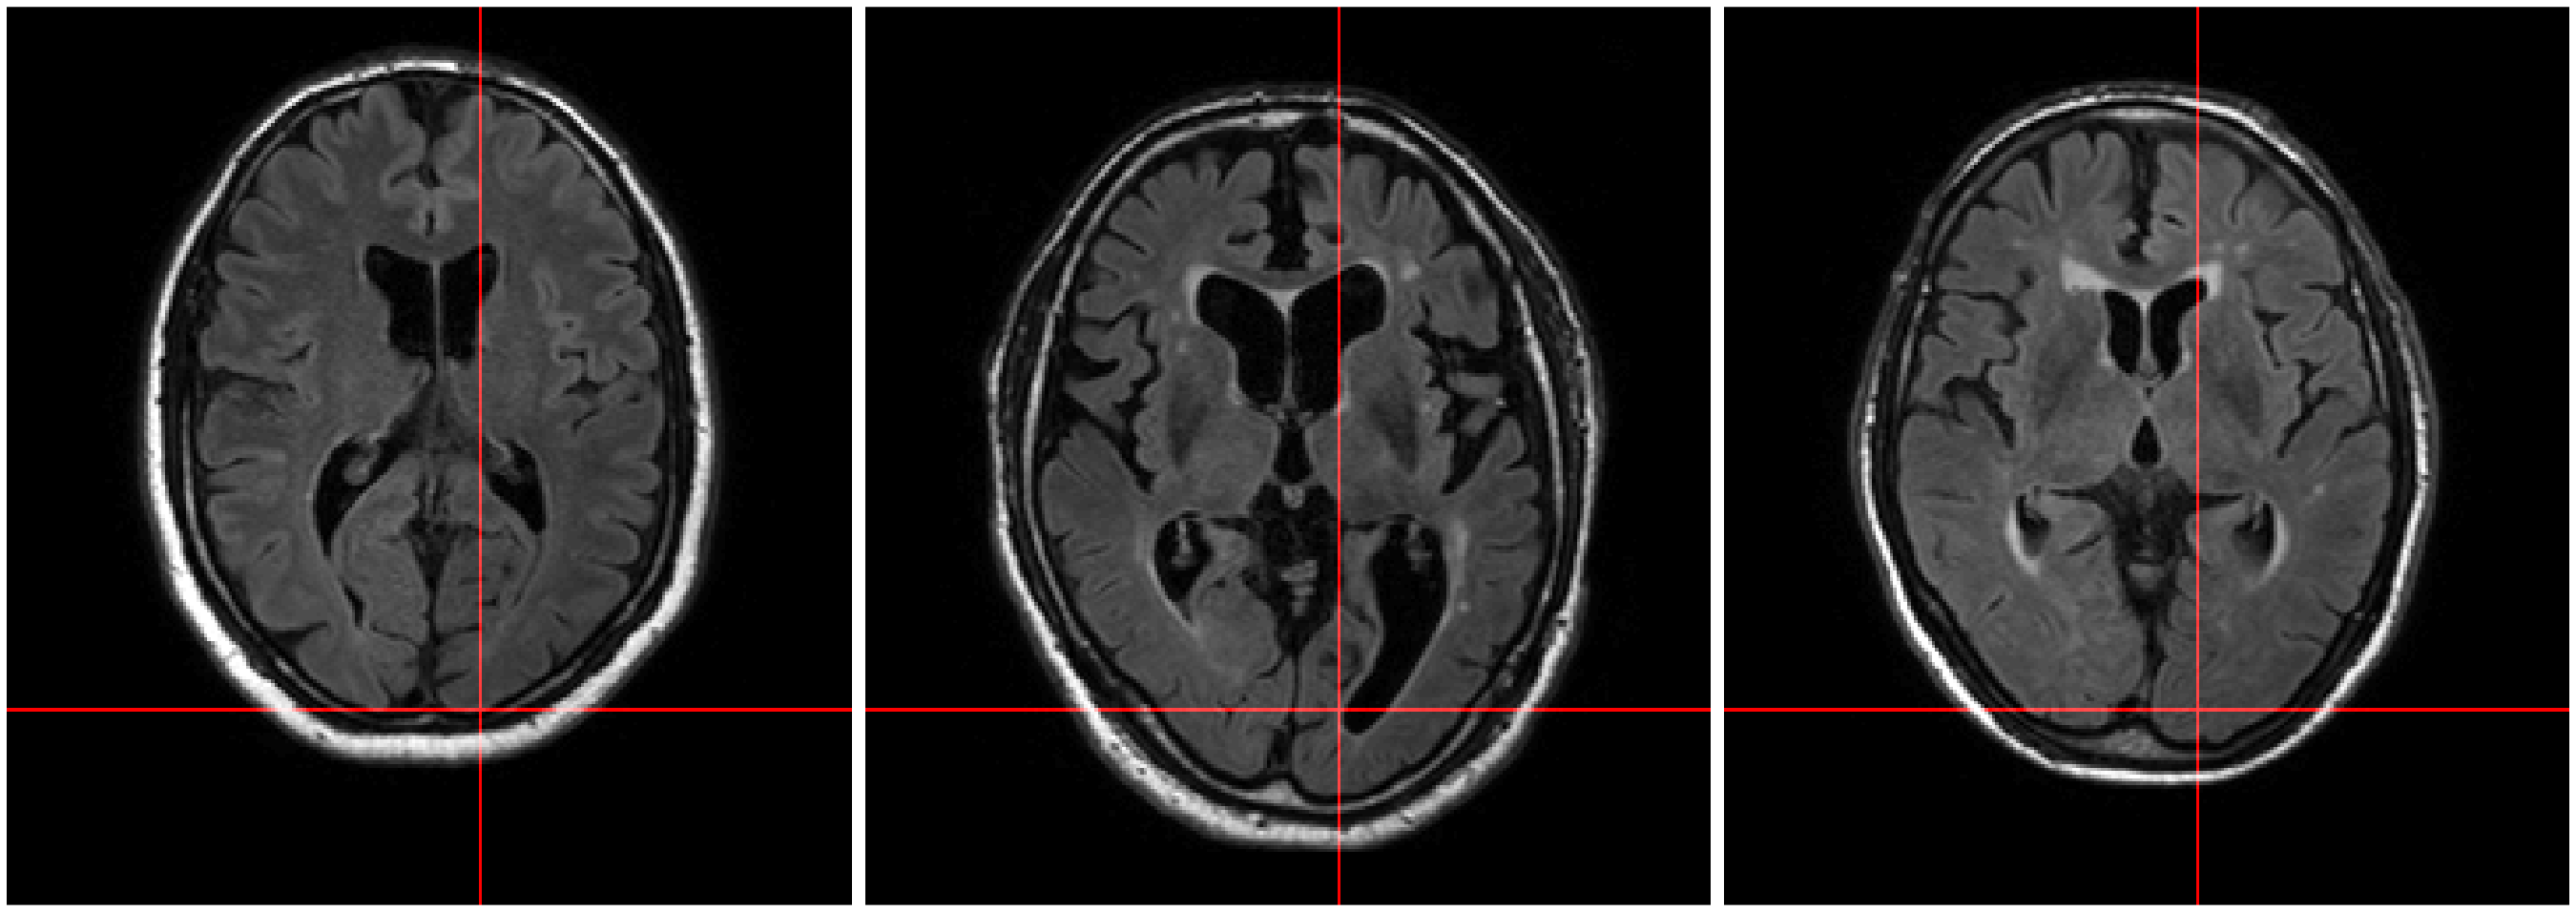
\includegraphics[width=0.9\textwidth]{pre-registration-1.png}
  }\\[0.5em]
  \subfigureoverl[white]{(b) Standard Space}{}{%
    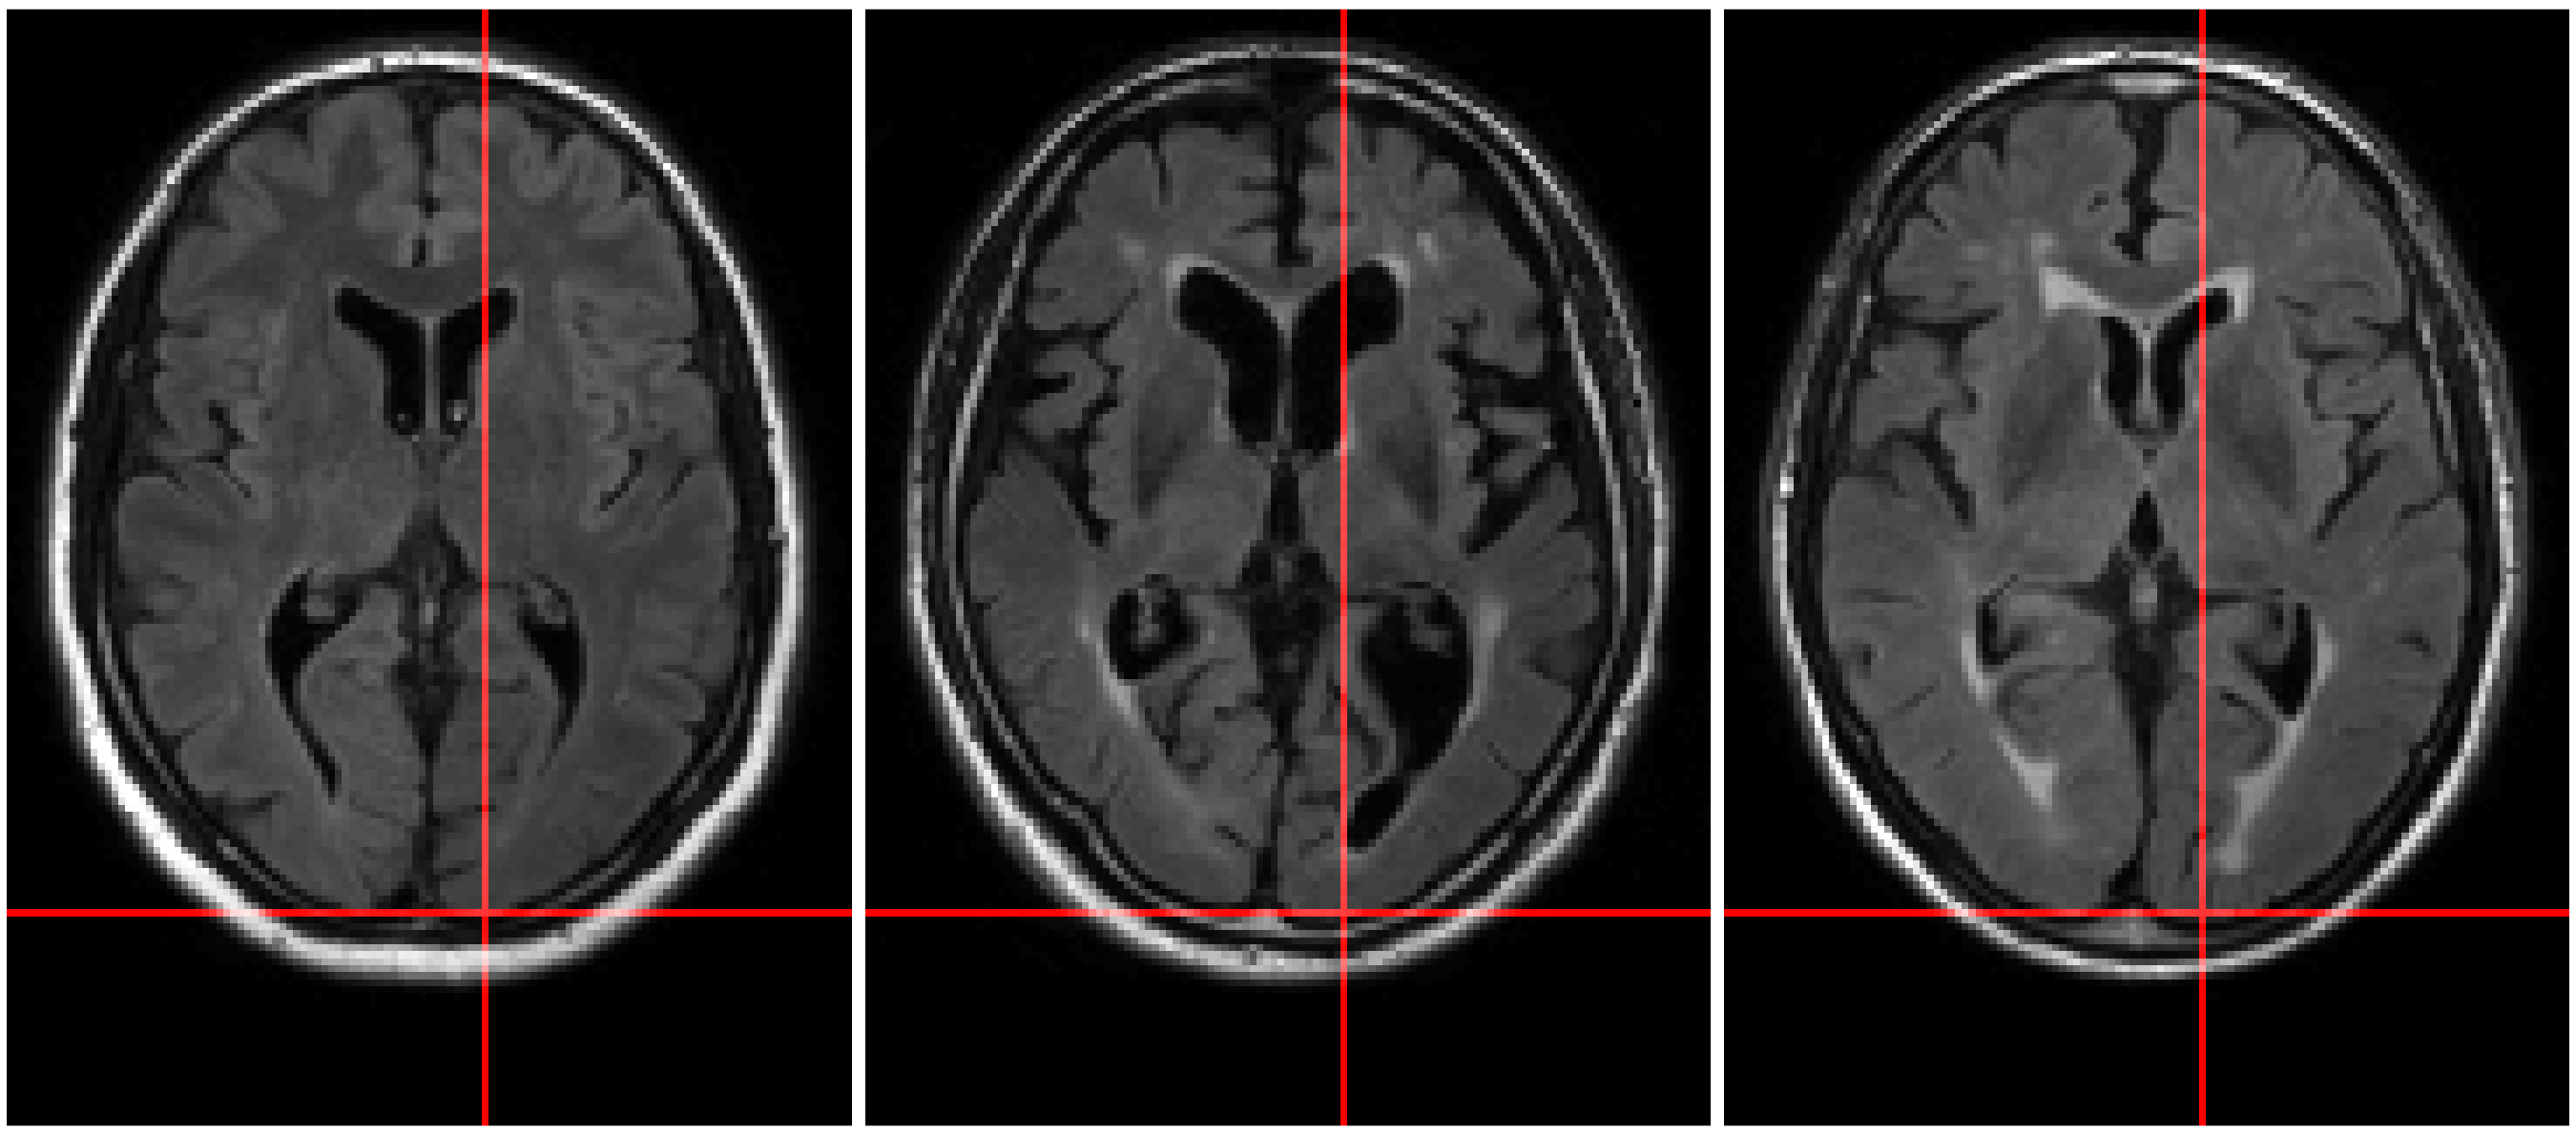
\includegraphics[width=0.9\textwidth]{pre-registration-2.png}
  }
  \caption{Example set of FLAIR MRI before and after registration to the MNI brain space.
    From~\cite{WMHSEG2017}.}%
  \label{fig:pre-registration}
\end{figure}
Parameters defining registration transforms are fit by
maximizing some measure of overlap between the images~\cite{Sotiras2013}.
Simple registration methods employ only affine transformations,
comprising a combination of translation, scaling, and shear transformations
(e.g.\ the \tool{FLIRT} tool~\cite{Jenkinson2002} in FSL).
The utility of these methods for neuroimage analysis is limited,
since there are often significant differences in brain anatomy between subjects.
Rather, most tools parametrize a spatial warping model,
permitting local nonlinear deformations to better match brain structures (e.g.\
cubic B-splines in FSL \tool{FNIRT}~\cite{Andersson2007},
discrete cosine transform in SPM \tool{Normalize}~\cite{Ashburner1997,Ashburner2005},
a general diffeomorphism in the SyN algorithm~\cite{Avants2008}).
While these models are more difficult to fit,
several robust algorithms have been released for general use,
with widespread acceptance (e.g.\ the toolboxes mentioned above).
A~\citeyear{Klein2009} comparison of 14 different methods
is a good resource on the subject~\cite{Klein2009},
while a more recent (\citeyear{Kazemi2014}) study
ranks the popular toolboxes SPM, FSL, and Brainsuite~\cite{Kazemi2014}.
\par
In the current work, registration is required during both training at testing.
During training, the model parameters $\bb(x)$ are estimated using
mutually aligned segmentation examples $\{\bY,\C\}$ in a standard brain space.
At test time (or for actual use), these parameter images
are transformed in the opposite direction from the standard space
to the native space of the current subject.
Since registration transforms are typically bijections -- i.e.\ invertible --
the second registration case can be estimated using the same method as the first, minimizing bias.
\par
Unlike other applications, it is not essential that perfect image registration is achieved here.
As noted by~\citeauthor{Harmouche2015}~\cite{Harmouche2015}, in smoothly varying models,
small registration errors can be expected to have a negligible impact.
Therefore, registration was not a primary focus of optimization in this work.
\par
While the registration component of the SPM8 \tool{Segment} feature~\cite{Ashburner2005}
was not among the top performing in the~\citeyear{Klein2009} study~\cite{Klein2009},
subsequent implementation revisions in SPM12%
\footnote{\hreftt{http://www.fil.ion.ucl.ac.uk/spm/software/spm12/SPM12_Release_Notes.pdf}}
called \tool{New Segment} have apparently improved results.
In the~\citeyear{Kazemi2014} study~\cite{Kazemi2014}, the SPM12 \tool{New Segment} method
achieved the highest Similarity Index of all methods on real (IBSR~\cite{IBSR}) data.
\par
Furthermore, the SPM module has several other features amenable to this work.
First, unlike many other registration algorithms,
the objective function does not require source and target images to have the same contrast.
This is helpful, since no suitable FLAIR template image is available for use as a target.%
\footnote{One FLAIR template is available in~\cite{Winkler2012};
  however, this was generated using SPM5, so using it
  would compound any registration biases associated with the older method.}
Second, it is simple to invoke the SPM modules via the command line or \matlab\ scripts;
this facilitates smooth integration of this tool in the pipeline.
Third, it is possible to save previously estimated registration transformations,
and apply them in the forward or reverse directions efficiently.
This can save significant time during cross validation,
since the estimated parameter images $\bm{\b}(x)$ must eventually be transformed
to the native space of every subject.
Finally, the SPM \tool{New Segment} model additionally estimates the bias field during execution
with high accuracy, saving an additional step (cf.~\S~\ref{s:pre-bias}, below).
For all these reasons, the registration performed by SPM \tool{New Segment}
was used throughout this work.
After satisfactory visual inspection of all training set images,
no other registration tools were investigated.
The default brain space of this module is MNI.
\par
The algorithm underlying \tool{New Segment} combines several models
in a unified probabilistic framework~\cite{Ashburner2005}.
Graylevels are modelled using a mixture of Gaussians,
parameterized by means $\bm{\mu}$ and covariances $\bm{\Sigma}$ (for-multi-image compatibility);
potential bias field is modelled using a discrete cosine transform,
parameterized by a vector $\bm{b}$;
spatial tissue priors in MNI space are deformed according to a similar discrete cosine transform,
parameterized by a vector $\bm{a}$~\cite{Ashburner1999}.
The parameters of each sub-model are optimized using expectation maximization
-- i.e.\ iteratively maximizing the likelihood of each parameter set,
given the data (input images), while fixing the others, until convergence.
The deformation field defined by the optimal $\bm{a}$ then gives
the transformation from MNI space to native space,
which can be inverted as needed.
%%%%%%%%%%%%%%%%%%%%%%%%%%%%%%%%%%%%%%%%%%%%%%%%%%%%%%%%%%%%%%%%%%%%%%%%%%%%%%%%%%%%%%%%%%%%%%%%%%%%
\section{Bias Correction}\label{s:pre-bias}
As noted in \S~\ref{ss:autochallenges}, bias field (\textsc{aka} intensity inhomogeneity),
is a smoothly varying intensity variation artifact common in MRI.
The sources of bias field artifact include
inhomogeneities in the magnetic field and RF coils used for pulse transmission and signal sensing,
as well as non-ideal magnetic properties of the imaged object~\cite{Vovk2007}.
The field and coil related sources are more significant at clinical field strengths.
These can be corrected prospectively, though techniques for doing so are limited,
and often a small bias field continues to corrupt acquired images~\cite{Vovk2007}.
Therefore, retrospective correction has been the subject of much research.
\par
Similar to image registration,
several widely accepted algorithms for estimating and correcting bias field have emerged.
The N3 algorithm~\cite{Sled1998}, subsequently updated to N4(ITK)~\cite{Tustison2010}
and integrated in the FreeSurfer toolbox%
\footnote{\hreftt{https://surfer.nmr.mgh.harvard.edu/}}
is perhaps the most popular, as it makes minimal assumptions about the image.
This method aims to sharpen the image histogram by dividing the image by an estimated bias field,
parameterized by B-splines for smoothness.
As noted above, the SPM \tool{New Segment} model~\cite{Ashburner2005}
includes integrated bias field estimation and correction,
and models the field using a discrete cosine transform.
The FSL \tool{Segment} feature also estimates bias field
in a similar overall model to SPM \tool{New Segment},
except the tissue prior probability maps in SPM are replaced with a Markov Random Field Model,
as described in~\cite{Zhang2001}.
Again, two reviews with quantitative performance comparisons
provide a good reference of other proposed algorithms,
including a comprehensive review in~\citeyear{Belaroussi2006}~\cite{Belaroussi2006}
and a comparison of mainly popular methods in~\citeyear{Ganzetti2016}~\cite{Ganzetti2016}.
\par
In the~\citeyear{Ganzetti2016} comparison~\cite{Ganzetti2016},
the authors note that the SPM and FSL models -- which include segmentation --
outperformed the N3 algorithm~\cite{Sled1998} and another non-segmenting method~\cite{Dawant1993}.
These results are consistent with
the advantages of unified generative models described in \S~\ref{sss:prior-models}
and discussed in~\citetitle{Ashburner2005}~\cite{Ashburner2005}.
Specifically, the estimation of both bias field and tissue segmentation are each improved
if the other is already known.
Rolling these tasks into a single EM-fitted model allows
alternating conditional estimates to converge on better results overall.
\par
Bias field estimation was not a primary focus of this work.
Therefore, due to the better performance over N3/4,
and the advantages already afforded by SPM \tool{New Segment} for registration noted above,
this model was employed for bias correction throughout this work.
No other bias field correction tools were investigated.
Figure~\ref{fig:pre-bias} shows a FLAIR image with conspicuous bias field,
the bias field estimated by SPM, and the corrected image.
\par
\begin{figure}
  \centering
  \begin{subfigure}{0.3\textwidth}
    \centering
    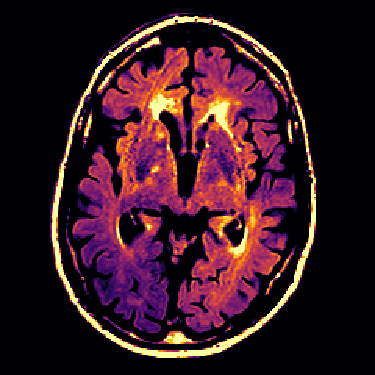
\includegraphics[height=1.5\sliceheight]{pre-bias-1.png}
    \caption{Raw FLAIR}
  \end{subfigure}
  \begin{subfigure}{0.3\textwidth}
    \centering
    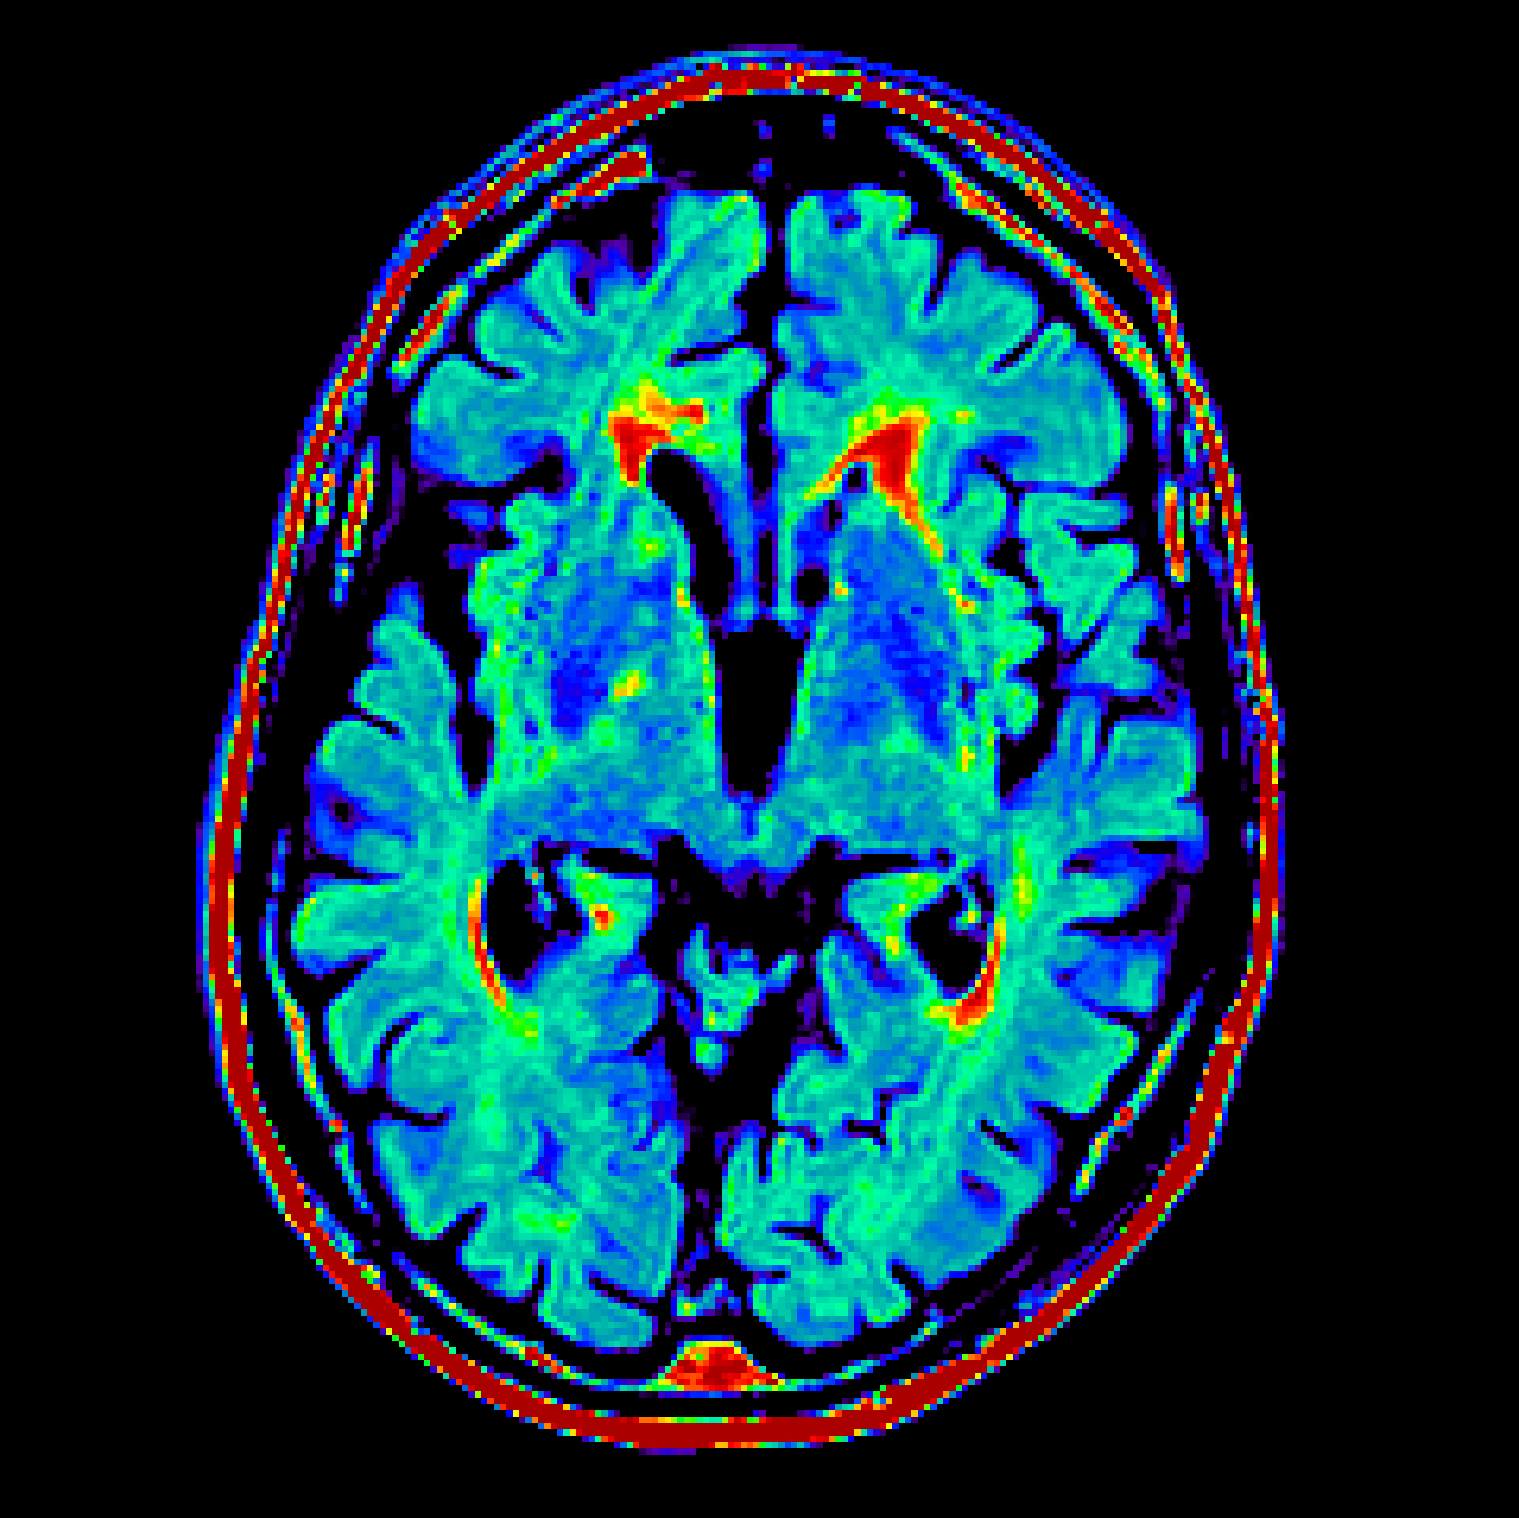
\includegraphics[height=1.5\sliceheight]{pre-bias-2.png}
    \caption{Bias-corrected FLAIR}
  \end{subfigure}
  \begin{subfigure}{0.30\textwidth}
    \centering
    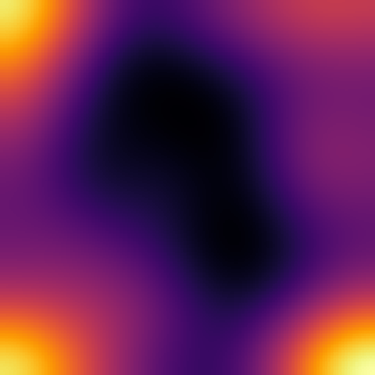
\includegraphics[height=1.5\sliceheight]{pre-bias-3.png}
    \caption{Estimated bias field}
  \end{subfigure}
  \begin{subfigure}{0.04\textwidth}
    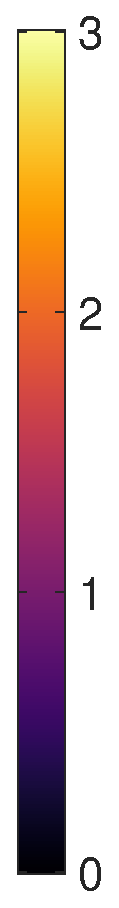
\includegraphics[height=1.5\sliceheight]{cmap-pre-bias}
    \\\vphantom{(x)}
  \end{subfigure}
  \caption{Example bias correction. From~\cite{WMHSEG2017}. Best viewed in colour.}%
  \label{fig:pre-bias}
\end{figure}
%%%%%%%%%%%%%%%%%%%%%%%%%%%%%%%%%%%%%%%%%%%%%%%%%%%%%%%%%%%%%%%%%%%%%%%%%%%%%%%%%%%%%%%%%%%%%%%%%%%%
\section{Graylevel Standardization}\label{s:pre-ystd}
The flexibility of image contrast in MRI is a double-edged sword.
This feature, in addition to properties of spatial encoding during acquisition,
preclude direct interpretation of image graylevels as a tissue property.
As a result, the same brain region in the same subject may be assigned a different graylevel
depending on the MRI sequence time constants, scanner, and spatial acquisition protocol.
For automated analysis of MRI images, therefore, standardization of image graylevels is required.
\par
Graylevel standardization can be achieved using a univariate transformation
$\uptau:y\mapsto\tilde{y}$, defined as
\begin{equation}
  \tilde{y} = \uptau(y),
\end{equation}
where $\uptau$ is monotonic, and considers characteristics of the input image,
such as basic graylevel statistics or the histogram.
The histogram of an image represents the number of occurrences of each graylevel in the image.
Normalizing the histogram by the total number of voxels $X$
yields the the probability mass function (PMF) $f_{\sy}(y)$,
\begin{align}
  f_{\sy}(y) &= \frac{1}{X}h_{\sy}(y)\nonumber\\
             &= \frac{1}{X}\sum_{i=1}^{X}
    \begin{cases}
      1 & Y(x_i) = y\\
      0 & Y(x_i) \ne y.\\
    \end{cases}
\end{align}
The cumulative density function (CDF) $F_{\sy}(y)$ is the cumulative sum of $f_{\sy}(y)$,
\begin{equation}
  F_{\sy}(y) = \sum_{\gamma=y_{\min}}^{y} f_{\sy}(\gamma).
\end{equation}
The PMF of an MRI can be decomposed into the contributions of each constituent tissue,
as shown in Figure~\ref{fig:simflairplot}.
This is the fundamental principle underlying mixture models.
% (cf.~\S~\ref{ss:priorproposed}).
The goal of standardization is therefore to align these sub-distributions as closely as possible.
\par
Previously proposed methods of standardizing MRI intensities include the following:%
\footnote{This section considers only univariate standardization methods,
  since only FLAIR intensities are used in this work.}
\begin{itemize}
  \item \textbf{Range Matching:}
  The simplest approach to standardization involves
  rescaling the data using the minimum and maximum intensities,
  \begin{equation}
    \uptau(y) = \frac{y-y_{\min}}{y_{\max}-y_{\min}}.
  \end{equation}
  Naively, this method is very susceptible to corruption by outliers.
  For more robustness, $y_{\min}$ and $y_{\max}$ can be defined using intensity quantiles
  -- e.g.\ $[\epsilon_1,1-\epsilon_2]$.
  However, selection of an appropriate $\epsilon_2$ for WMH segmentation is difficult,
  since WMH typically constitute only the top 1\% of the total brain volume.
  Furthermore, differences in image contrasts are not considered by this approach.
  \item \textbf{Statistical standardization:}
  Another simple but popular approach uses the first and second order moments of the PMF,
  \begin{equation}
    \uptau(y) = \frac{y-\mu_{\sy}}{\sigma_{\sy}}.
  \end{equation}
  As with range matching, variable image contrasts are not well modelled by this method.
  \item \textbf{Histogram equalization:}
  Histogram equalization transforms the image PMF to a uniform distribution,
  thereby distributing image intensities equally across the available range.
  The desired transform  is defined as the CDF of the input image
  (cf.~\cite{Gonzalez2006} for derivation),
  \begin{equation}
    \uptau(y) = F_{\sy}(y).
  \end{equation}
  The chief assumption of histogram equalization for standardization is
  that input images contain consistent amounts of each tissue class.
  In MRI with WMH, this assumption may not be valid;
  however, this technique may still have value.
  \item \textbf{Histogram matching:}
  Histogram matching is similar to histogram equalization, except that
  the output PMF is not uniform, but some other specified distribution, $f_{\tilde{\sy}}$.
  This transform is defined as
  the function composition of the input CDF and the inverse target CDF,
  \begin{equation}
    \uptau(y) = {F_{\tilde{\sy}}}^{-1}\big(F_{\sy}(y)\big).
  \end{equation}
  While histogram matching yields images with different contrast characteristics than
  histogram equalization, these two methods are equivalent in their ability
  to standardize image graylevels
  (cf.~\ref{s:hm-vs-he} for an illustration and experimental evidence).
  \item \textbf{Nyul standardization:}
  In~\cite{Nyul1999,Nyul2000},~\citeauthor{Nyul1999} proposed a method for
  intensity standardization which has subsequently been used in other works. %__JK__find these
  This method defines $\uptau$ with piecewise linear segments
  connecting the $Q$ quantiles of the input PMF $q$, with quantiles of a target PMF $r$,
  \begin{equation}
    \uptau(y) = r_i + \left(y-q_i\right)
      \left(\frac{r_{i+1}-r_i}{q_{i+1}-q_i}\right),\quad y\in[q_i,q_{i+1}].
    \end{equation}
  However, it can be shown that this transformation is
  a non-uniform trapezoidal Riemann approximation of true histogram matching,
  which performs worse in terms of intensity standardization.%
  \footnote{This result is presented and supported with experiments in~\cite{Knight2017}.} % chktex 42
  \item \textbf{Regional characteristics:}
  Decorrelating variation in intensities from variability in anatomical content
  is a central challenge in intensity standardization.
  One solution is to define the image-specific transformation using characteristics
  from a more anatomically consistent brain region.
  This is the approach employed by~\citeauthor{Shinohara2014}
  in the so-called white stripe method~\cite{Shinohara2014}.
  In the current work, this region, denoted $\X_{\uptau}$,
  can be defined in MNI space using tissue priors (Figure~\ref{fig:tpm-3}),
  anatomical label maps, or any other method of selecting a subset of voxels.
\end{itemize}
% ==================================================================================================
\subsection{Quantifying Standardization}
While the major advantages and challenges to several graylevel standardization methods
have been briefly noted, it remains to explore the utility of each experimentally.
In the current work, the goal of this step is to maximize the separation of the two classes.
This can even be maximized voxel-wise, due to the characteristics of the VLR model.
Therefore, an intermediate objective function $\Z$ should be defined
which quantifies the degree of separation of the two classes.%
\footnote{Alternatively, the entire pipeline can be executed under cross validation
  and overall performance compared between standardization methods.
However this does not consider potential interactions
between the standardization method and tunable downstream parameters.}
This objective function can then be used to optimize
any tunable parameters in each of the transforms
-- e.g.\ $\bm{\epsilon}$, $Q$, $\X_{\uptau}$ --
and also to select the best overall method.
\par
Two such functions are proposed.
The first is discrete, and inspired by the Zero-Crossing Rate~\cite{Kedem1986}.
It measures the number of class transitions in the sorted feature data $\tilde{\Y}_s$,
as shown in Figures~\ref{fig:jsep-diff-1} and~\ref{fig:jsep-diff-2}.
With $\C_s$ as the class labels after sorting by the feature $\tilde{\Y} = \uptau(\Y)$,
the objective function $\Z_{\Delta}$ is defined as
\begin{equation}
  \Z_{\Delta} = \sum_{n=1}^{N-1}
     \begin{cases}
      1 & \C_s^{n} \ne \C_s^{n+1}\\
      0 & \C_s^{n}  =  \C_s^{n+1}.
    \end{cases}%
    \label{eq:zsep-diff}
\end{equation}
This function is discrete and bounded, as in
$\Z_{\Delta}\in\mathbb{Z}\left[1,\lfloor\frac{N}{2}\rfloor\right]$%
\footnote{The lower bound can be zero if one class is not observed.}
and the lower bound is optimal -- i.e.\ $\Z_{\Delta}$ should be minimized.
\par
The second function is continuous, and inspired by probability theory.
It measures the relative overlap of class distributions,
$p(\tilde{y}\mid c=1)$ and $p(\tilde{y}\mid c=0)$,
estimated using kernel smoothing,
as shown in Figures~\ref{fig:jsep-conv-1} and~\ref{fig:jsep-conv-2}.
This objective function $\Z_{\star}$ can be defined as
\begin{equation}
  \Z_{\star} = \int_{\tilde{y}_{\min}}^{\tilde{y}_{\max}}
    \frac{\min\{p(\psi \mid c=1), p(\psi \mid c=0)\}}
         {\max\{p(\psi \mid c=1), p(\psi \mid c=0)\}}\d\psi,
    \qquad p(\psi \mid c)
      \approx \sum_{\tilde{y}\in\{\tilde{\Y}\mid c\}}\delta(\psi-\tilde{y}) \star G_{\sigma}(\psi).%
      \label{eq:zsep-conv}
\end{equation}
where $G_{\sigma}(\psi)$ is a Gaussian convolution kernel with width $\sigma$.
This function is continuous and bounded, as in
$\Z_{\Delta}\in\left[0,1\right]$,
and the lower bound is again optimal.
\par
\begin{figure}
  \centering
  \foreach \i/\desc in {% % chktex 1
    1/{with overlapping classes},%
    2/{with barely separable classes},%
    3/{with easily separable classes}%
  }{%
    \begin{subfigure}{\plotwidth}
      \includegraphics[width=\textwidth]{jsep-diff-\i}
      \caption{$\Z_{\Delta}$ \desc}%
      \label{fig:jsep-diff-\i}
    \end{subfigure}
    \begin{subfigure}{\plotwidth}
      \includegraphics[width=\textwidth]{jsep-conv-\i}
      \caption{$\Z_{\star}$ \desc}%
      \label{fig:jsep-conv-\i}
    \end{subfigure}
  }
  \caption{Illustration of potential separability objective functions
    using three sets of sample data (black circles).
  $\Z_{\Delta}$ counts the class changes in the sorted feature data
  (numbered red lines).
  $\Z_{\star}$ computes the ratio of the overlap between class data distributions (red area)
  to the total data distribution (blue areas).}%
  \label{fig:jsep}
\end{figure}
% ==================================================================================================
\subsection{Supervised Standardization}
It is not hard to see that it should be possible to estimate an
optimal graylevel standardization transform using the training data.
That is, a \textit{supervised graylevel standardization}.%
\footnote{To the best of this author's knowledge, such a technique has never been proposed.}
If $\Z$ is differentiable, then this optimization can be performed
using gradient descent, or similar methods.
Unfortunately, neither of the above objective functions $\Z$ were reasonably differentiable,
but many other optimization paradigms which do not require
differentiable objective functions could be used
-- e.g.\ reinforcement learning~\cite{Mnih2015} or Bayesian Optimization~\cite{Shahriari2016}.
Due to time constraints, these methods were not explored.
%%%%%%%%%%%%%%%%%%%%%%%%%%%%%%%%%%%%%%%%%%%%%%%%%%%%%%%%%%%%%%%%%%%%%%%%%%%%%%%%%%%%%%%%%%%%%%%%%%%%
\section{Pre-Processing Summary}
In summary, to train the VLR model,
a set of labelled training images must first be registered to a standard brain space (MNI).
This is achieved using the SPM \tool{New Segment} tool, which also produces bias corrected images.
Next, image intensities are standardized using a graylevel transformation,
to be determined in Chapter~\ref{ch-exp}.
Training then proceeds to fit the VLR model parameters, as described in Chapter~\ref{ch-vlr}.
\par
At test time, SPM \tool{New Segment} is used again to
correct the bias field and estimate the registration to MNI space for a given input image.
However, the inverse transform is now used to warp the parameter images $\bb(x)$
from MNI space to the native space.
This transformation of the smooth parameter images prior to inference is preferable
to transforming the detailed label image afterwards.
The VLR model then predicts the WMH class label, followed by the necessary post-processing steps.
% --------------------------------------------------------------------------------------------------
% ==================================================================================================
%%%%%%%%%%%%%%%%%%%%%%%%%%%%%%%%%%%%%%%%%%%%%%%%%%%%%%%%%%%%%%%%%%%%%%%%%%%%%%%%%%%%%%%%%%%%%%%%%%%%

  %%%%%%%%%%%%%%%%%%%%%%%%%%%%%%%%%%%%%%%%%%%%%%%%%%%%%%%%%%%%%%%%%%%%%%%%%%%%%%%%%%%%%%%%%%%%%%%%%%%%
% ==================================================================================================
% --------------------------------------------------------------------------------------------------
\chapter{Voxel-Wise Logistic Regression}\label{ch-vlr}
This section presents the proposed classification model
-- Voxel-wise Logistic Regression (VLR) --
in more detail, and explores the specific parameters and regularization strategies
requiring optimization.
\par
To review, the predicted lesion class label image $\hat{C}(x)$ is defined
using the subject-specific features $\bY(x) = {[1,Y^1(x),\dots,Y^\sk(x)]}^T$
and the corresponding model weights $\bb(x) = {[\b^0(x),\b^1(x),\dots,\b^\sk(x)]}^T$,
\begin{equation}
\hat{C}(x) = \frac{1}{1+e^{-\eta(x)}},\qquad\eta = {\bb(x)}^T\bm{Y}(x).%
\label{eq:eq:vlrmodel}
\end{equation}
While the implementation used for experimentation in this work
uses only one feature image ($K=1$), the FLAIR graylevel,
the derivations and discussions below will maintain generality for any selection of features.
%%%%%%%%%%%%%%%%%%%%%%%%%%%%%%%%%%%%%%%%%%%%%%%%%%%%%%%%%%%%%%%%%%%%%%%%%%%%%%%%%%%%%%%%%%%%%%%%%%%%
\section{Model Fitting}\label{ss:modelfitting}
Fitting the VLR model involves estimating $\bb$ for each voxel $x$.
This requires some training data:
feature vectors from a population of $N$ observations $\bY(x) = \{\bY_1(x),\dots,\bY_{\sn}(x)\}$,
and the corresponding labels $\C(x) = \{C_1(x),\dots,C_{\sn}(x)\}$.
As in many probabilistic models,
parameter estimation involves maximizing the likelihood of the model, given this data --
i.e.\ maximum likelihood estimation (MLE).
% ==================================================================================================
\subsection{Challenges}\label{ss:vlr-chmle}
Three major challenges emerge during model fitting.
These challenges involve contradictions between prior knowledge
and the fitted model using the available training data.
That is, these challenges could all be overcome by a more complete training set,
but this is rarely available.
The three challenges are:
\begin{enumerate}
  \item\label{chmle:separable} \textbf{Separable classes:}
  When data from two classes are perfectly separable,
  the MLE-fitted logistic model can approach a step-function -- i.e.\ $\b^k\rightarrow+\infty$.
  This implies that on either side of a specific graylevel threshold,
  the model is either 100\% confident in predicting the healthy class,
  or 100\% confident in predicting the lesion class.
  In fact, no threshold is ever so perfect,
  and instead a level of uncertainty should be maintained around the decision boundary.
  These two cases are illustrated in Figure~\ref{fig:chmle-sep}.
  \item\label{chmle:sparse} \textbf{Sparsely observed lesion class:} 
  Since WML are often distributed in consistent locations,
  many brain regions contain no lesions across the entire training dataset.
  These voxels will be termed ``healthy training'' voxels, and denoted $\X_{h}$.
  In some locations, this is expected
  (e.g.\ the GM, since by definition WMH manifest in the WM),
  while in others, prior knowledge predicts lesions will eventually be observed
  (e.g.\ the rest of the WM).
  As illustrated in Figure~\ref{fig:chmle-noles},
  the MLE-fitted model may not maintain the ability to predict $\hat{c} = 1$ in such locations,
  regardless of the features.
  However, the ability to predict lesion should be maintained in many of these locations.
  \item\label{chmle:noisy} \textbf{Smooth parameter images:} 
  It is assumed that similar locations will contain similar training data,
  yielding smooth parameter images.
  If this assumption is sometimes invalid,
  parameter images could contain noise or discontinuities,
  creating artifacts in estimated lesion class images.
\end{enumerate}
\begin{figure}
  \centering
  \begin{subfigure}{\plotwidth}
    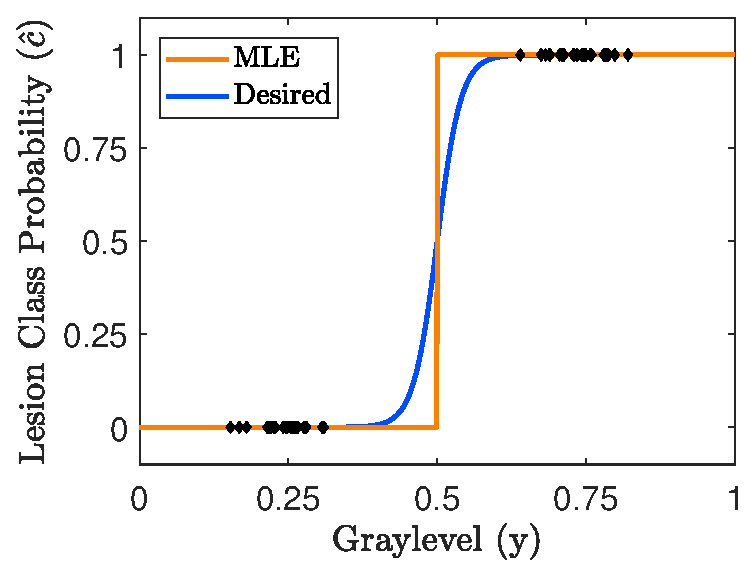
\includegraphics[width=\textwidth]{chmle-sep}
    \caption{Separable classes}%
    \label{fig:chmle-sep}
  \end{subfigure}
  \begin{subfigure}{\plotwidth}
    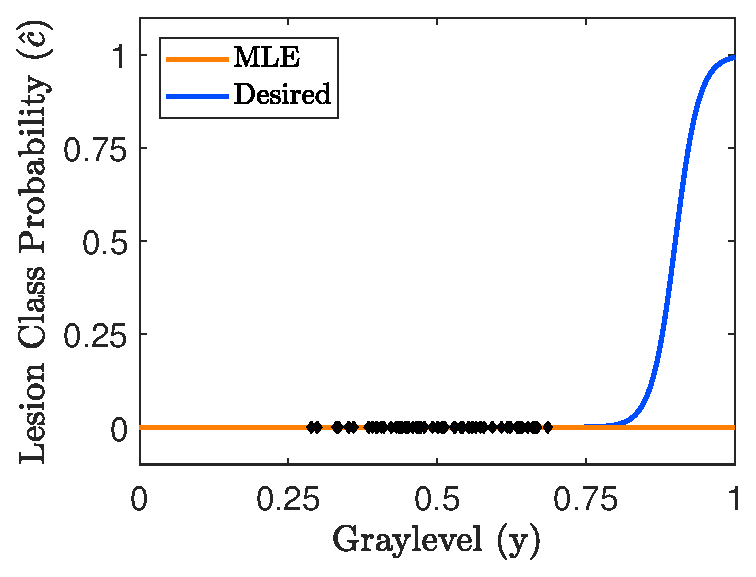
\includegraphics[width=\textwidth]{chmle-noles}
    \caption{No lesions}%
     \label{fig:chmle-noles}
   \end{subfigure}
  \caption{Challenges encountered during estimation of a logistic model.}%
  \label{fig:chmle}
\end{figure}
% ==================================================================================================
\subsection{Maximum Likelihood Estimation}
Each parameter vector $\bb(x)$ is considered completely independent.
Doing so greatly simplifies model fitting, but does not address the challenges described above.
These must instead be addressed using regularization strategies,
as discussed below in \S~\ref{s:vlr-reg}.
In this section, ML estimation of independent parameter vectors $\bb$ is developed.
For clarity, only a single voxel is considered -- i.e.\ $y$ from $Y(x)$, etc.
\par
As note above, the optimal $\bb$ for each independent voxel can be resolved using MLE.
If the training data are also assumed to be independently observed,
then the likelihood (conditioned on the data) is defined from binomial theory as
\begin{align}
  L(\bb\mid\C,\bY) &= \prod_{n=1}^{N} {P(c=1\mid\by_n,\bb)}^{c_n}
                              \left(1-{P(c=1\mid\by_n,\bb)}^{1-c_n}\right)\nonumber\\
                   &= \prod_{n=1}^{N} \Big[\hat{c}_n^{\en c_n}
                                   \left(1-\hat{c}_n^{\en 1-c_n}\right)\Big].%
  \label{eq:likelihood}
\end{align}
For computational reasons,
it is simpler and asymptotically equivalent to maximize the log-likelihood,
\begin{align}
  \L(\bb) &= \log{ \prod_{n=1}^{N} \Big[\hat{c}_n^{\en c_n}
                                \left(1-\hat{c}_n^{\en 1-c_n}\right)\Big] }\nonumber\\
          &= \sum_{n=1}^{N} \Big[ c_n \log \hat{c}_n + (1-c_n) \log (1-\hat{c}_n) \Big] \nonumber\\
          &= \sum_{n=1}^{N} \Big[ c_n \bb^T\by_n - \log (1+e^{\bb^T\by_n}) \Big].%
  \label{eq:loglikelihood}
\end{align}
The optimal $\bb$ is therefore resolved by maximizing the log-likelihood,
\begin{align}
  \bb^* &= \underset{\bb}{\arg\max}\en\L(\bb)\nonumber\\
        &= \underset{\bb}{\arg\max}\en\sum_{n=1}^{N}
             \Big[ c_n \bb^T\by_n - \log (1+e^{\et\bb^T\by_n}) \Big]%
  \label{eq:argmaxmle}
\end{align}
% ==================================================================================================
\subsection{Iterative Updates}
Estimation of $\bb^*$ can be performed using iterative optimization,
using an initial estimate $\bb^{(0)}$ and an update term $\Delta\bb^{(t)}$,
\begin{equation}
  \bb^{(t+1)} \leftarrow \bb^{(t)} + \alpha\thinspace\Delta\bb^{(t)},%
  \label{eq:update}
\end{equation}
where $\alpha$ is a small valued learning rate parameter.
There are many possible definitions of $\Delta\bb$,
including simply the gradient of $\L(\bb)$, denoted $\nabla_{\bb}\L$.
However, it can be shown that $\L(\bb)$ is convex, so higher order update equations can be used.
The work by~\citeauthor{Minka2003}~\cite{Minka2003} compares several options,
including Newton's method (and variants),
conjugate gradient, iterative scaling (and variants), and dual optimization.%
\footnote{Matlab code available at \hreftt{https://github.com/tminka/logreg/}}
For small feature dimensionality ($K$), performance differences among the options were small.
Classic Newton updates gave a good balance between memory requirements and computational order,
so they are used.
\par
If the gradient $\nabla_{\bb}\L$ and Hessian matrix $\nabla^2_{\bb}\L$ are defined as
\begin{align}
  \nabla_{\bb}\L   &= \left[\begin{array}{c}
                        \frac{\d L}{\d\b^1}\\\vdots\\\frac{\d L}{\d\b^\sk}
                      \end{array}\right],%
  \label{eq:llgradient0}\\
  \nabla^2_{\bb}\L &= \left[\begin{array}{ccc}
                        \frac{\d^2 L}{\d\b^1\d\b^1}   & \cdots & \frac{\d^2 L}{\d\b^1\d\b^\sk}\\
                                               \vdots & \ddots & \vdots \\
                        \frac{\d^2 L}{\d\b^\sk\d\b^1} & \cdots & \frac{\d^2 L}{\d\b^\sk\d\b^\sk}
                      \end{array}\right]%
  \label{eq:llhessian0},
\end{align}
then the Newton update is given by
\begin{equation}
  \Delta\bb = -{\nabla^2_{\bb}\L}^{-1}\nabla_{\bb}\L.%
  \label{eq:newtonmle}
\end{equation}
In the current model, the gradient is given by 
\begin{equation}
  \nabla_{\bb}\L = \sum_{n=1}^{N} \by_n\left(c_n - \hat{c}_n\right),%
  \label{eq:llgradient}
\end{equation}
and the Hessian by
\begin{equation}
  \nabla^2_{\bb}\L = \sum_{n=1}^{N} \by_n{\by_n}^T \left(c_n - \hat{c}_n\right).%
  \label{eq:llhessian}
\end{equation}
Substituting (\ref{eq:llgradient}) and (\ref{eq:llhessian}) into (\ref{eq:newtonmle}),
the explicit update $\Delta\bb$ for (\ref{eq:update}) is obtained.
At each iteration, $\Delta\bb^{(t)}$ is re-computed,
and the process continues until some convergence criterion is satisfied.
% ==================================================================================================
\subsection{Simplification}\label{ss:vlr-simple}
It is not necessary to complete the above procedure for all voxels in the standardized space.
Instead, only voxels in the expected location of the brain need to be computed;
such voxels can be selected using a binary ``brain mask'', denoted $M(x)$.
More details about the brain mask used in this work can be found in \S~\ref{ss:brainmask}.
Moreover, since the parameters of each voxel are estimated independently,
this can also be computed in parallel.
The details of this implementation are presented in \S~\ref{s:parallelfit},
after incorporation of the regularizations described in the next section.
\par
Finally, the model has so far been derived in general terms,
so that any choice of feature set $\by$ can be used.
However, with only one feature -- the FLAIR graylevel --
it is possible to reparameterize the sigmoid argument as
\begin{align}
  \bb^T\by &= \b^0 + \b^1 y^1\nonumber\\
           &= s(y-\tau)
           \qquad\begin{cases}
             s = \b^1\\
             \tau = -\frac{\b^0}{\b^1}
           \end{cases}.%
  \label{eq:reparameterize}
\end{align}
In this form, the parameters $\tau$ and $s$ emerge
as a graylevel threshold and a slope parameter, respectively.
Specifically, when $y = \tau$,
the predicted probability of lesion is $\hat{c} = \tfrac{1}{1+e^{0}} = 0.5$,
so $\tau$ controls the location of the class discrimination,
as shown in Figure~\ref{fig:reparam-t}.
Similarly, the $s$ parameter defines the sensitivity of the logistic function to $y$,
as shown in Figure~\ref{fig:reparam-s}.
By contrast, varying the original parameter $\beta^1$ with $\beta^0$ constant
(Figure~\ref{fig:reparam-b1}) results in correlation of these characteristics.
These new parameters, and the corresponding images $\mathcal{T}(x)$ and $\mathcal{S}(x)$,
are therefore salient descriptors of the predictive model.
\begin{figure}
  \centering
  \begin{subfigure}{\plotwidth}
    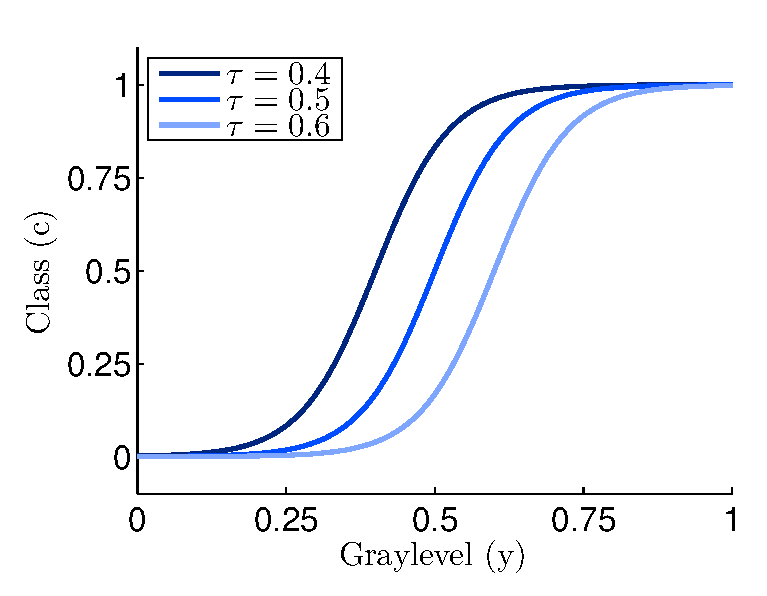
\includegraphics[width=\textwidth]{reparam-t}
    \caption{Vary $\tau$ with $s = 16$ constant.}%
    \label{fig:reparam-t}
  \end{subfigure}
  \begin{subfigure}{\plotwidth}
    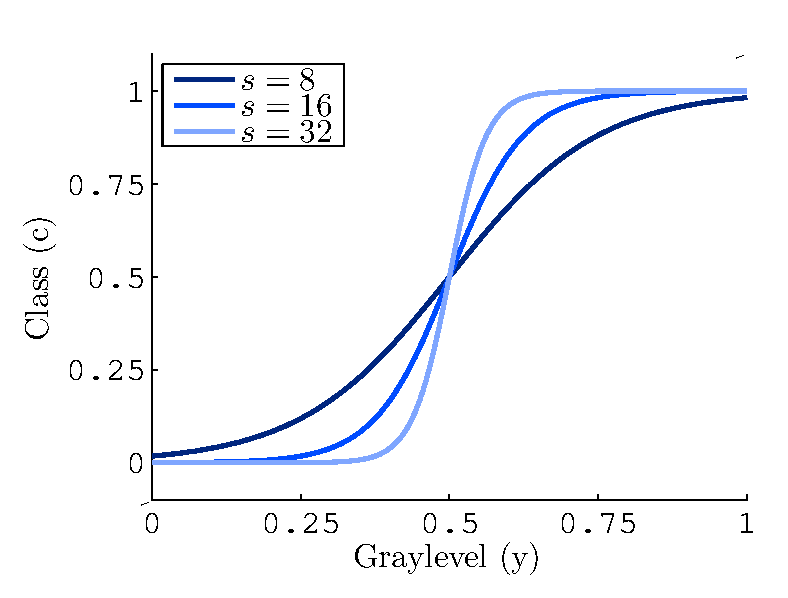
\includegraphics[width=\textwidth]{reparam-s}
    \caption{Vary $s$ with $\tau = 0.5$ constant.}%
    \label{fig:reparam-s}
  \end{subfigure}
  \begin{subfigure}{\plotwidth}
    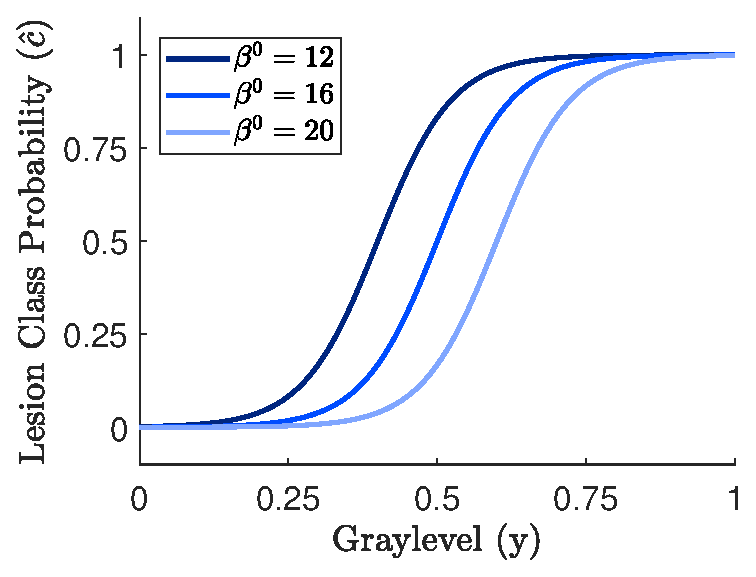
\includegraphics[width=\textwidth]{reparam-b0}
    \caption{Vary $\b^0$ with $\b^1 = 16$ constant.}%
    \label{fig:reparam-b0}
  \end{subfigure}
  \begin{subfigure}{\plotwidth}
    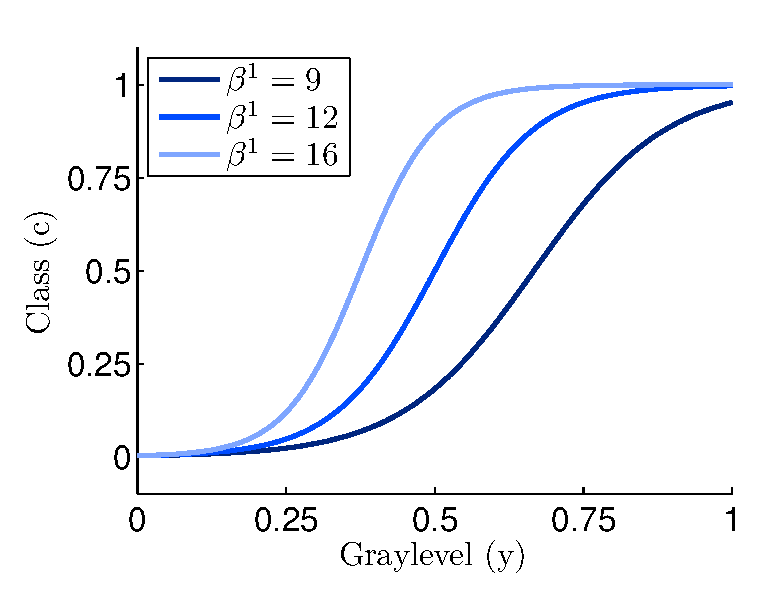
\includegraphics[width=\textwidth]{reparam-b1}
    \caption{Vary $\b^1$ with $\b^0 = -6$ constant.}%
    \label{fig:reparam-b1}
  \end{subfigure}
  \caption{Effect of varying the logistic model parameters.}%
  \label{fig:reparam}
\end{figure}
%%%%%%%%%%%%%%%%%%%%%%%%%%%%%%%%%%%%%%%%%%%%%%%%%%%%%%%%%%%%%%%%%%%%%%%%%%%%%%%%%%%%%%%%%%%%%%%%%%%%
\section{Regularization}\label{s:vlr-reg}
Regularizations are
methods of injecting prior knowledge about the expected model into the optimization.
Assuming voxel-wise independence of model parameters requires the use of regularization strategies
to solve the challenges outlined in \S~\ref{ss:modelfitting}.
Several regularization methods are explored below.
% ==================================================================================================
\subsection{Data Augmentation}\label{ss:vlr-reg-aug}
Noting the central role of training data in each of the challenges,
methods of artificially increasing the training dataset size
may be particularly useful in solving them.
Data augmentation has long been used in machine learning tasks with limited training data,
and there are several methods of generating synthetic data.
In low dimensional input/output spaces,
random sampling of fitted class-conditional posterior distributions
can produce reasonable samples with known labels~\cite{Tanner1987}.
In higher dimensional problem spaces, however, imputation is more difficult~\cite{Goodfellow2014}.
For example, the space of potential $100\times100\times100$-sized images has $100^3$ dimensions
(one per voxel), yet only a small subspace represents plausible images.
Generating synthetic examples in this space is therefore challenging,
especially for segmentation tasks,
where the outputs have dimensionality roughly equal to the input.
\par
Alternatively, simple image manipulations can still afford model improvements~\cite{Krizhevsky2012}.
In segmentation tasks, both the input image(s) and the corresponding label images can be
translated, reflected, rotated, and perhaps resized,
thereby avoiding the generation of genuinely synthetic examples.
In the current work, reflections and small (one-voxel) translations
can be applied to the label and FLAIR images following registration to the MNI brainspace.
The potential benefits of this augmentation are explored in \S~\ref{ss:exp-reg}.
%__JK__ need also to define MNI before here...?
% ==================================================================================================
\subsection{Classic Regularization}\label{ss:vlr-reg-lambda}
The separable classes challenge is well-known in regression problems,
and a good solution is to penalize the magnitude of model parameters using the $L_p$-norm:
$\lambda\norm{\bb}_p$~\cite{Zou2005}.
It can be shown that $L_1$ regularization corresponds to a Laplacian prior on elements of $\bb$,
with scale parameter inversely proportional to $\lambda$
(equivalently, this assumes that the model error follows this distribution).
Similarly, $L_2$ regularization implies a Gaussian prior,
with standard deviation inversely proportional to $\lambda$~\cite{Zou2005}.
Model fitting which includes this prior-derived term is called
maximum a posteriori (MAP) estimation,
and the penalty can be appended to the objective function (\ref{eq:argmaxmle}), as in
\begin{align}
  \bb^* &= \underset{\bb}{\arg\max}\en\J(\bb) \nonumber\\
        &= \underset{\bb}{\arg\max}\en\L(\bb) - \lambda\norm{\bb}_p \nonumber\\
        &= \underset{\bb}{\arg\max}\en\sum_{n=1}^{N}
           \Big[ c_n \bb^T\by_n - \log (1+e^{\et\bb^T\by_n}) \Big] - \lambda\norm{\bb}_p%
  \label{eq:argmaxmap}
\end{align}
Due to its relatively large gradient near zero,
$L_1$ regularization is typically used to encourage sparsity in the feature weights
(i.e.\ $\b^k\rightarrow0$)~\cite{Tibshirani1996}.
This is not desirable in the current model,
since the feature (FLAIR graylevel) is known to be discriminative.
Moreover, the expansion of the $\norm{\bb}_1$ term
in the gradient of the objective function is not straightforward,
since it is non-differentiable at zero~\cite{Tibshirani1996,Lee2006}.
Conversely, $L_2$ regularization is more effective at limiting parameter magnitude
-- which is the current aim --
and the first and second order gradients of (\ref{eq:argmaxmap}) derive easily~\cite{Minka2003}.
For these reasons, only $L_2$ regularization is considered,
yielding the following change to the Newton update expression (\ref{eq:newtonmle}),
\begin{align}
  \Delta\bb &=-{\nabla^2_{\bb}\J}^{-1}\nabla_{\bb}\J \nonumber\\
            &=-{\left(\nabla^2_{\bb}\L-\lambda I\right)}^{-1}\left(\nabla_{\bb}\L-\lambda\bb\right)%
  \label{eq:newtonmap}
\end{align}
What remains is to select an appropriate value of $\lambda$.
This is explored experimentally in \S~\ref{ss:toyreg} using a toy model.
% ==================================================================================================
\subsection{Pseudo-Lesions}\label{ss:vlr-reg-pseudo}
The sparsely observed lesion class challenge is less common,
since discriminative models are rarely fit in the absence of one class altogether.
This occurs here because all voxels are modelled independently.
It is therefore tempting to simply sample features from the lesion class at other spatial locations
in order to fit the logistic model in the healthy training voxels,
similar to the approach by~\citeauthor{Schmidt2017a}.
However, as noted in \S~\ref{ss:autochallenges} and \S~\ref{sss:limits-flair},
WML are thought to have different intensities
in different brain regions~\cite{Sled2004,Stevenson2000},
and some locations will likely never contain any WMH.
Considering these facts, the use of deterministic synthetic lesion-class samples,
or ``pseudo-lesions'', could instead permit better use of prior knowledge about WMH.
These synthetic observations could be appended to the training data for each voxel
so as to minimally balance the training classes,
and act as a prior on the distribution of lesion-class features.
% This approach would not be subject to variations in the training data,
% and it would be feasible to consider the prior probability of healthy tissues
% (GM / WM / CSF) in the definition.
\par
If the same number of synthetic observations are appended to the training data for each voxel,
this is equivalent to appending a number of synthetic images to the training set.
The synthetic feature data are denoted
$\bV(x) = \{\bm{\gamma}_{1}(x),\dots,\bm{\gamma}_{\sv}(x)\}$.
It is assumed that the labels of all synthetic data are ``lesion'',
so the set of synthetic label images is simply denoted $\bm{1}(x)$.
The updated training set is therefore
$\bY_{\gamma}(x) = \{\bY(x),\bV(x)\}$, and $\bC_{\gamma}(x) = \{\bC(x),\bm{1}(x)\}$.
\par
Design of the synthetic image set $\bV(x)$ should be guided by prior knowledge.
For the same reasons as described above,
it is not possible to derive this knowledge from the training set.
Unfortunately, few other sources of structured information are available.
One reasonable approach could make use of healthy tissue prior probability images
(Figure~\ref{fig:tpm-3}), denoted $\rho(x)$.
Specifically, the expected intensity for the lesion class in each tissue
can be multiplied by the tissue probability image,
and the results summed to give the overall synthetic image,
\begin{equation}
  \gamma(x) = \gamma_{\gm{}}\cdot\rho_{\gm{}}(x)
            + \gamma_{\wm{}}\cdot\rho_{\wm{}}(x)
            + \gamma_{\csf{}}\cdot\rho_{\csf{}}(x)
\end{equation}
While WMH are not possible in either the GM or the CSF,
it is necessary to select a FLAIR graylevel
-- perhaps the maximum possible intensity --
to complete this model.
Additionally, such parameters will inevitably play a role
for subjects with imperfect registration or outlier anatomy.
The contributions of pseudo-lesions to model fitting
are explored experimentally in \S~\ref{ss:toyreg}.
%__JK__ should TPMs be introduced sooner?
\begin{figure}
  \centering
  \subfigureoverl[white]{(a) $\rho_{\gm{}}(x)$}{}{%
    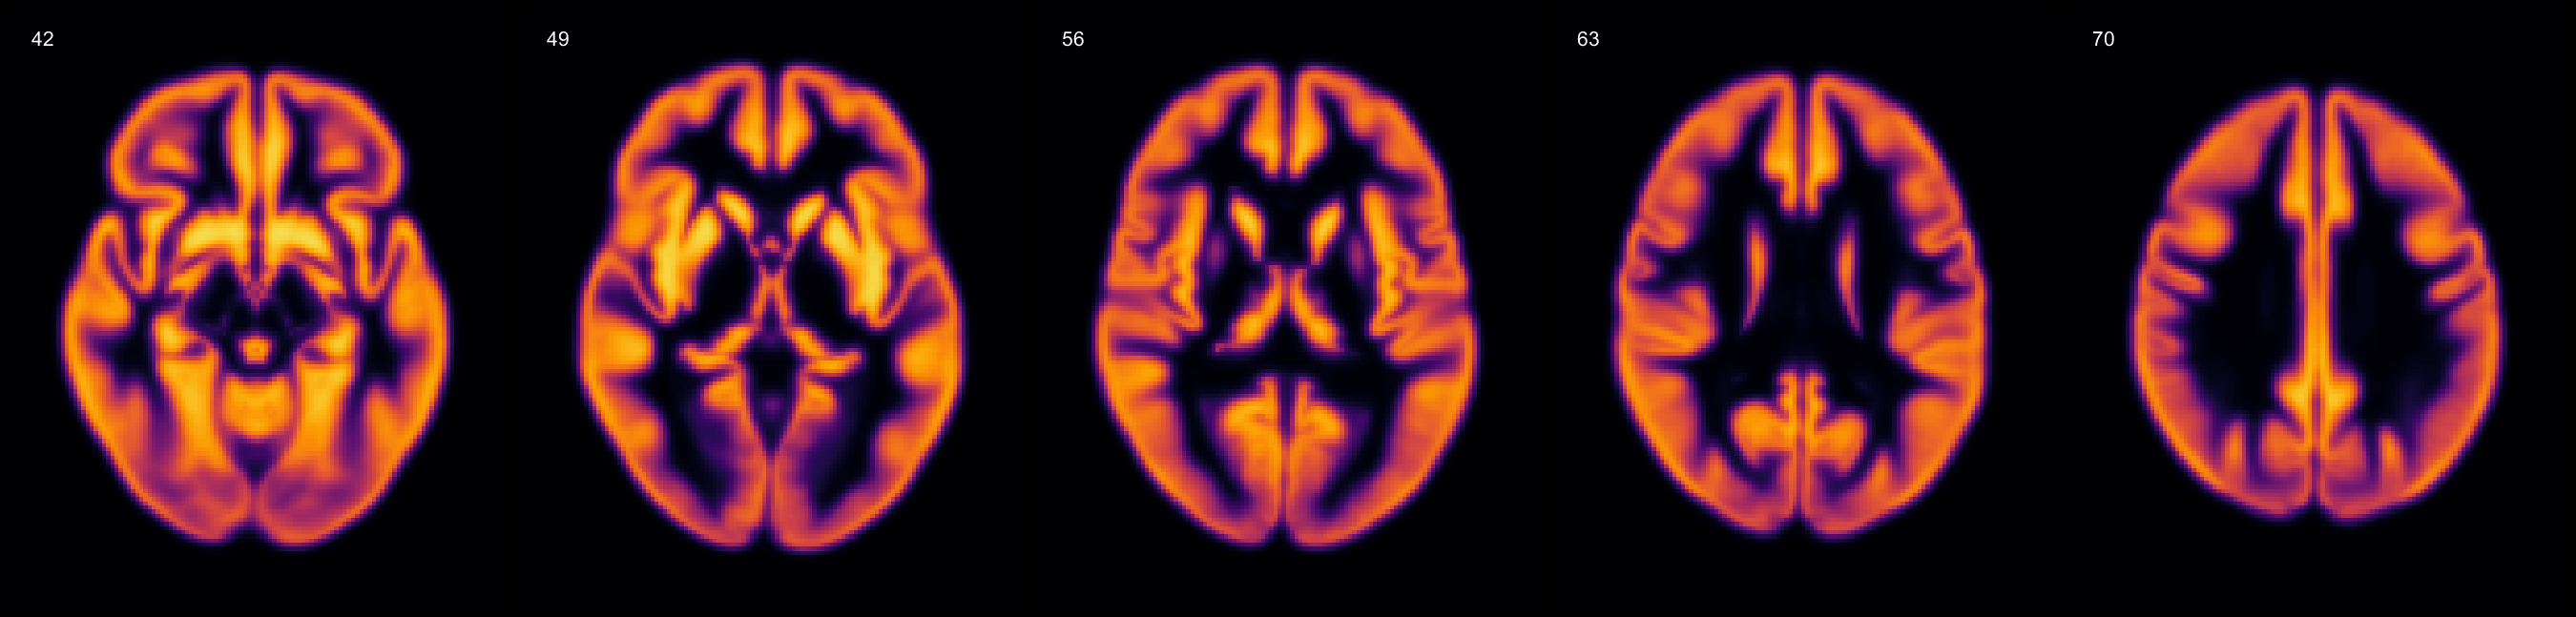
\includegraphics[height=\sliceheight]{tpm-gm.png}
    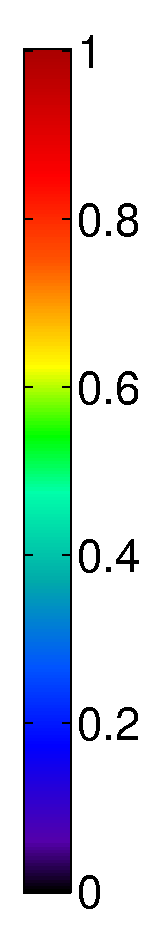
\includegraphics[height=\sliceheight]{cmap-tpm}%
  }\\[0.5em]
  \subfigureoverl[white]{(b) $\rho_{\wm{}}(x)$}{}{%
    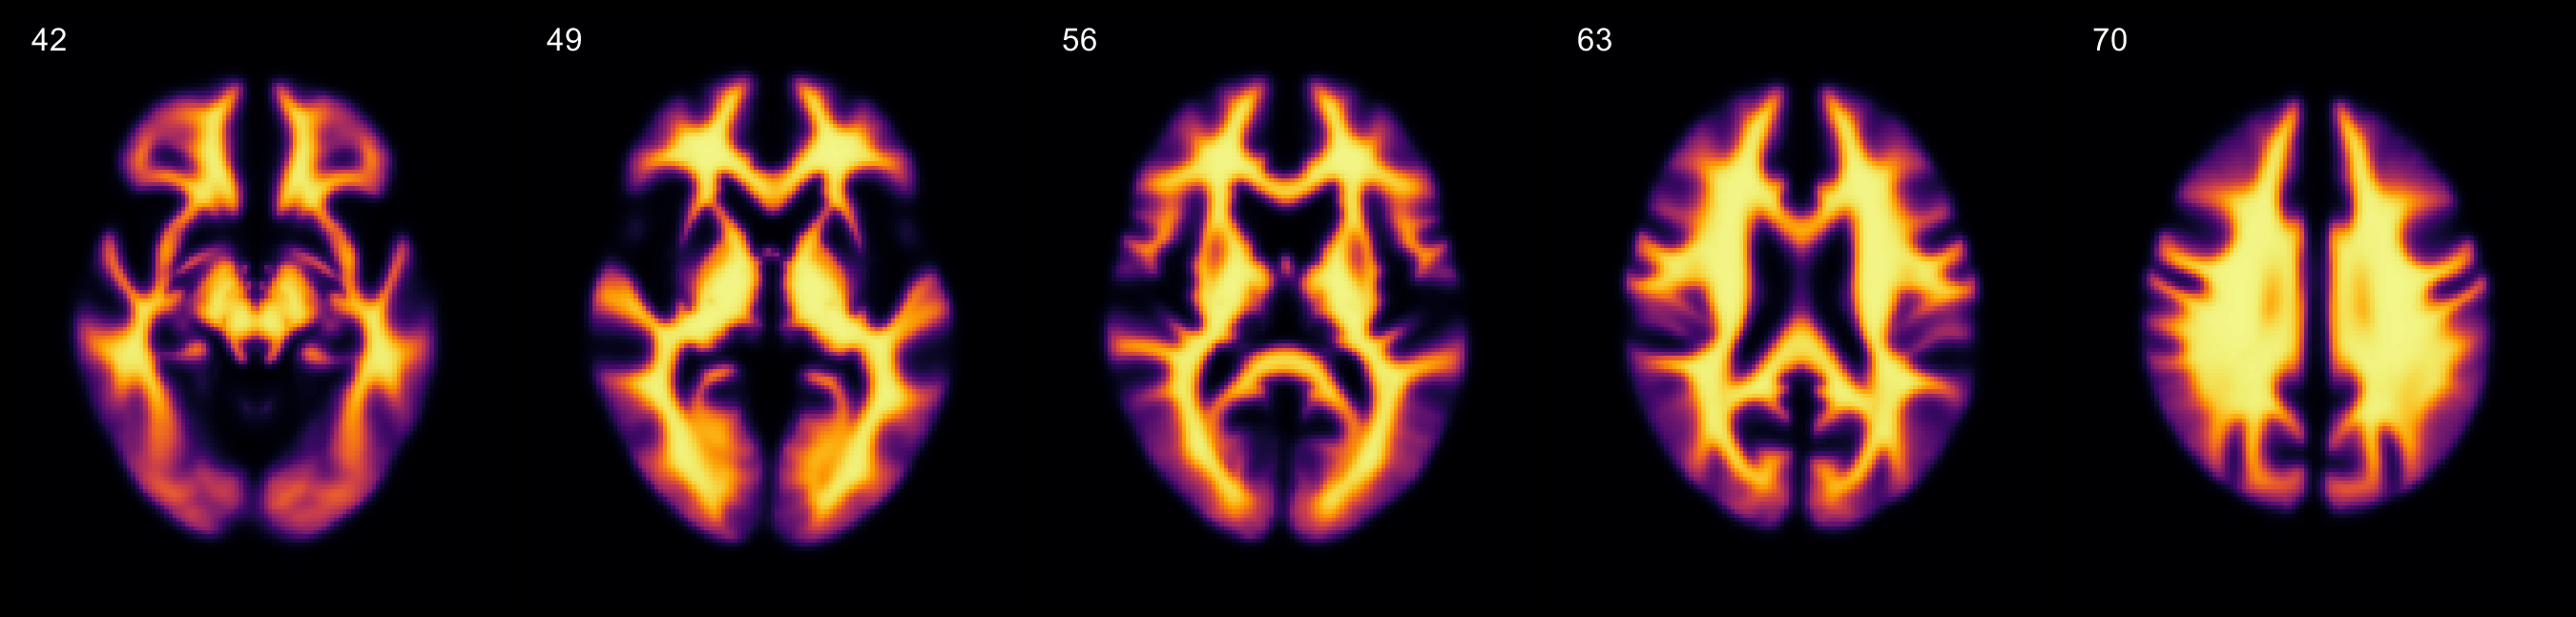
\includegraphics[height=\sliceheight]{tpm-wm.png}
    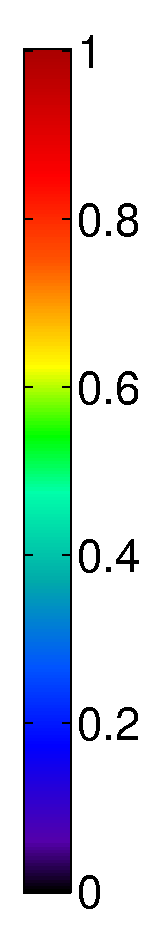
\includegraphics[height=\sliceheight]{cmap-tpm}%
  }\\[0.5em]
  \subfigureoverl[white]{(c) $\rho_{\csf{}}(x)$}{}{%
    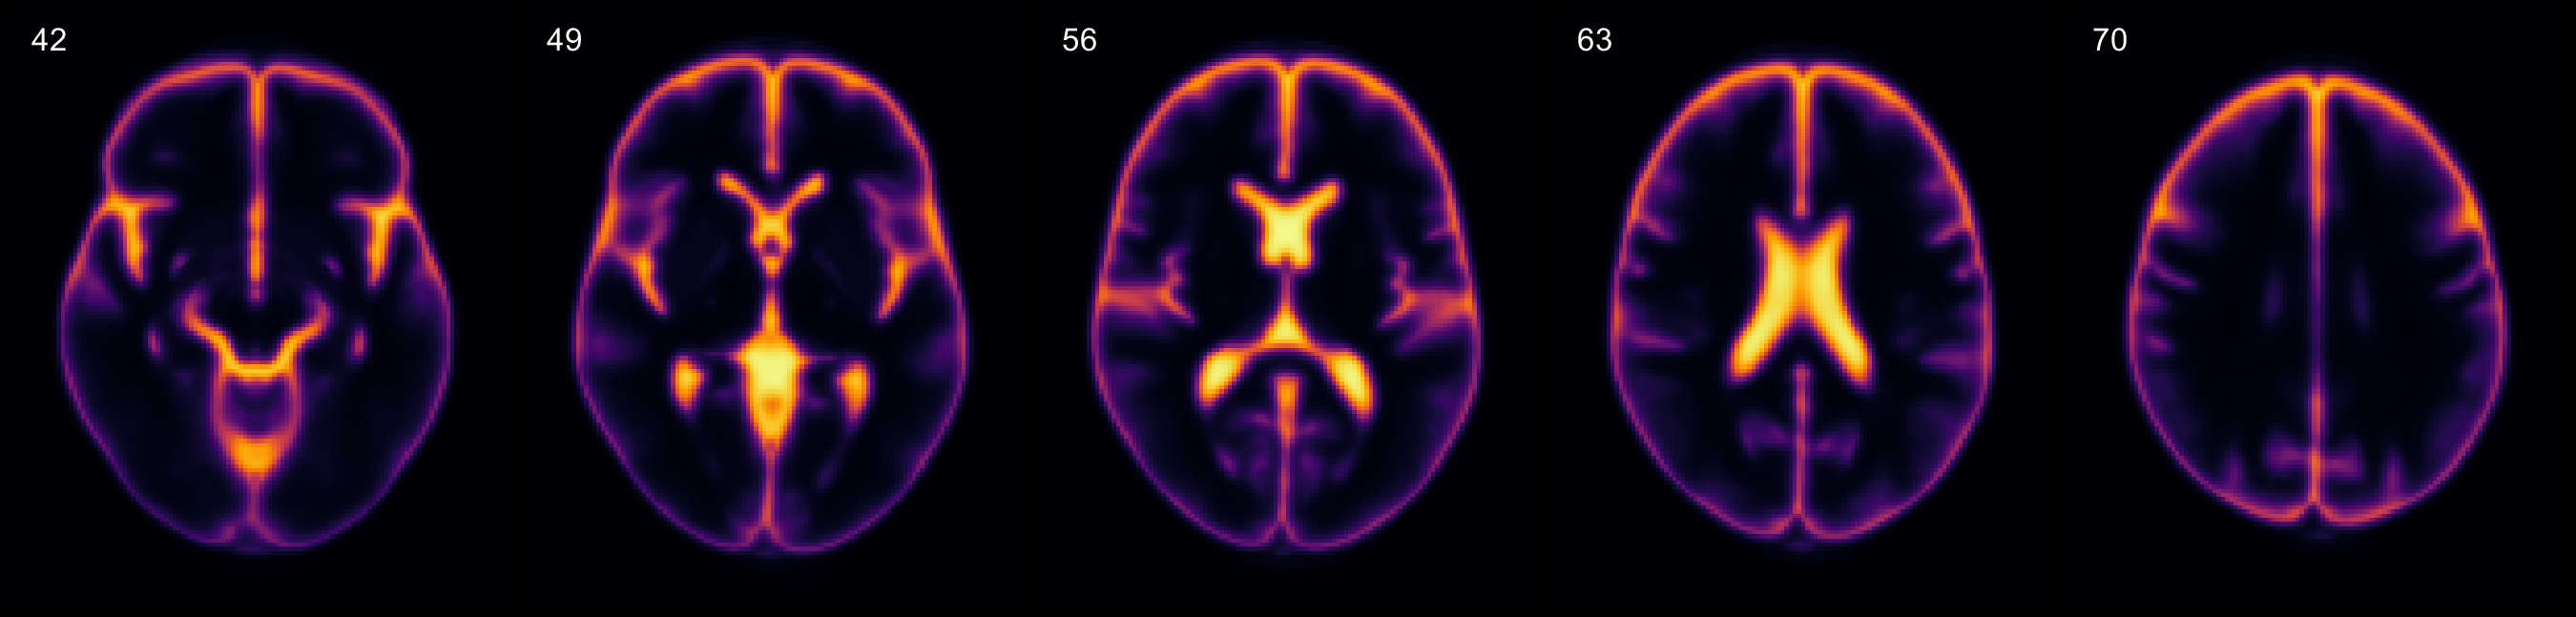
\includegraphics[height=\sliceheight]{tpm-csf.png}
    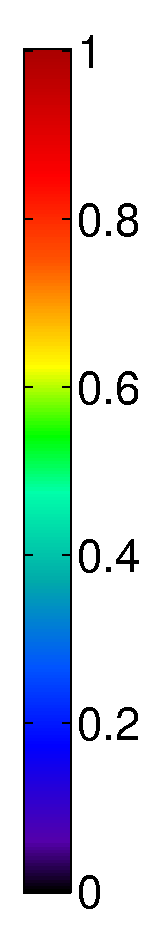
\includegraphics[height=\sliceheight]{cmap-tpm}%
  }
  \caption{Tissue prior probability images in MNI space.
    Derived from~\cite{Mazziotta2001}.}%
  \label{fig:tpm-3}
\end{figure}
% ==================================================================================================
\subsection{Parameter Image Smoothing}\label{ss:vlr-reg-smooth}
Finally, independent model fitting in every voxel risks yielding noisy parameter images.
The simplest solution to this problem involves
filtering the reconstructed parameter images after estimation.
A wide range of possible filters for this task exist,
and a selection of these are summarized in Table~\ref{tab:filters},
including the mutable parameters for each.
\begin{table}
  \centering
  \caption{Image filters considered for smoothing the estimated parameter images.}%
  \label{tab:filters}
  \begin{tabular}{llllc}
  	\toprule
  	Name      & Parameters            & Advantages                   & Disadvantages    &        Ref.         \\ \midrule
  	Gaussian  & width $\sigma$        & no artifacts                 & blurs edges      & \cite{Gonzalez2006} \\ % chktex 2
  	Median    & width $w$             & preserves edges              & square artifacts & \cite{Gonzalez2006} \\ % chktex 2
  	Bilateral & $\sigma_y$,$\sigma_x$ & balanced blurring and detail & Expensive        &  \cite{Tomasi1998}  \\ \bottomrule % chktex 2
  \end{tabular}
\end{table}
\par
An alternative solution might involve modelling the parameter images as a spatial function
(e.g.\ band-limited discrete cosine / Fourier transform).
However, there are two challenges with this approach.
First, deriving the update gradients for such a model would be challenging,
and their computation could significantly increase training time.
Second, such an encoding may introduce artifacts in the resulting parameter images.
Moreover, it is well known that frequency domain band-limiting
can be equivalently achieved by convolution (i.e.\ filtering)
in the spatial domain~\cite{Gonzalez2006}.
Therefore, only conventional filtering is explored in this work (cf.~\S~\ref{}).
%__JK__ define this reference in ch-exp
%__JK__ address MRFs for smoothing here?
%%%%%%%%%%%%%%%%%%%%%%%%%%%%%%%%%%%%%%%%%%%%%%%%%%%%%%%%%%%%%%%%%%%%%%%%%%%%%%%%%%%%%%%%%%%%%%%%%%%%
\section{Post-Processing}\label{s:vlr-post}
At this point, the motivation and details of the proposed VLR model have been presented,
in addition to the preprocessing steps required to satisfy its assumptions.
The last component of a segmentation pipeline typically includes post-processing. 
In principle, this step aims to incorporate any additional knowledge of the problem
which has not been considered in upstream elements.
Here, these include the connected morphology of WML, and the minimum lesion size.
Discussions of these topics, however, would assume that the label image is already binary,
whereas the output from the VLR model is probabilistic.
Therefore, the first post-processing step
thresholds the WMH class probability to give a ``hard'' classification:
$\hat{c}\rightarrow \hat{c}^{\circ}$
This also facilitates comparison with manual segmentation masks, which are usually binary.
%__JK__ better notation for this hard label: \hat{c}^{\circ}? 
% ==================================================================================================
\subsection{Thresholding}\label{ss:vlr-thr}
If the assumptions of any probabilistic model are valid,
then the ``hard'' classification is straightforward:
\begin{equation}
  \hat{c}^{\circ} = \underset{\omega}{\arg\max}\en p(\omega\mid\by,\bb)\quad\forall \omega.
\end{equation}
In a 2-class logistic regression model, this simplifies to thresholding:
\begin{equation}
  \hat{c}^{\circ} = \begin{cases} 0 & \hat{c} < \pi_c \\ 1 & \hat{c} \ge \pi_c \end{cases},
\end{equation}
with $\pi_c = 0.5$.
However, since these assumptions are often only partially true,
most models are able to achieve better agreement with manual segmentations
using a different threshold $\pi_c$ for the WMH class.
In fact several of the freely available toolboxes (cf.~\S~\ref{sss:wmhsegtoolboxes})
permit a user-specified threshold which can be optimized for the user's data.
During model validation,
this parameter should be optimized using the training data for each cross validation fold.
It is also prudent to illustrate the sensitivity of the model to this parameter, using either 
a plot of performance versus threshold~\cite{Steenwijk2013}, or
a precision-recall (PR) curve~\cite{Arbelaez2011}.
In the current work, both these techniques are employed:
$\pi_c$ is optimized on the fly, and a PR curve is given after.
% ==================================================================================================
\subsection{Minimum Lesion Size}\label{ss:vlr-minx}
With finite image resolution and appreciable noise in MRI,
lesions appearing as only a few connected voxels are indistinguishable from image noise,
even by human experts.
Such potential lesions are therefore not included in radiologists assessment of WML.
Accordingly, most WMH segmentation algorithms employ
a minimum-connected-voxels exclusion criterion during post-processing.
Connectedness can be defined in 2D or 3D,
and consider only direct adjacency or diagonal connections too.
Most works employ the most liberal definition: 26-connectedness,
which considers all $3\times3\times3-1=26$ candidates surrounding a given voxel in 3D.
Ideally, the number of required connected voxels will adapt to the image resolution,
and correspond to a minimum lesion volume.
Typical volumes range from about $\mathrm{x}_{\min}^{c} = $
$3.5$ mm\textsuperscript{3} in~\cite{Steenwijk2013,Fartaria2015}, to 
$9.0$ mm\textsuperscript{3} in~\cite{Yoo2014,Elliott2013}.
\par
In the current work, the inclusion of a minimum lesion size rule is explored.
The optimal value for $\mathrm{x}_{\min}^{c}$ is resolved experimentally
during each cross validation fold, and the resulting values compared with the above conventions.
Additionally, the gains in performance afforded by this step are quantified.
% __JK__ I was going to include the MRF in this section too,
% but since I really didn't investigate these in any great detail,
% I was hoping to omit this overall. I would save a lot of time running experiments,
% and also they never seemed to improve performance (in fact, the opposite).
% It would require a lot more tinkering to get some good results,
% and I don't think I'm really in that position right now.
% __JK__
% \subsection{Connected Morphology of WML}
% \par...\par
% Preliminary qualitative investigations into lesions with these characteristics
% suggested that errors in this area were not a significant problem for the model.
%%%%%%%%%%%%%%%%%%%%%%%%%%%%%%%%%%%%%%%%%%%%%%%%%%%%%%%%%%%%%%%%%%%%%%%%%%%%%%%%%%%%%%%%%%%%%%%%%%%%
% __JK__ what to do about this ugly \hat{c}^{\circ} notation from above?
%        Keep for all references to the hard labelled images? :(
%%%%%%%%%%%%%%%%%%%%%%%%%%%%%%%%%%%%%%%%%%%%%%%%%%%%%%%%%%%%%%%%%%%%%%%%%%%%%%%%%%%%%%%%%%%%%%%%%%%%
\section{Model Summary}
In summary, the proposed algorithm uses graylevel features
to train a logistic regression model for each voxel independently -- Voxel-Wise Logistic Regression.
In order to train the VLR model,
a set of labelled training images must first be registered to a standard brain space (MNI).
This is achieved using the SPM Segment tool, which also produces bias corrected images.
Next, image intensities are standardized using a graylevel transformation,
to be determined in the next section.
The parameter images $\bb(x)$ are then computed using iterative MAP estimation,
with Newton updates and an augmented dataset.
These images are smoothed to reflect prior knowledge.
Finally, the optimal probability threshold $\pi_c$ and  minimum lesion size $\mathrm{x}_{\min}^{c}$
are estimated using the training data.
This completes the training phase.
\par
At test time, SPM Segment is used again to
correct the bias field and estimate the registration to MNI space for a given input image.
However, the inverse transform is now used to warp the parameter images $\bb(x)$
from MNI space to the native space.
This transformation of the smooth parameter images prior to inference is preferable
to transforming the detailed label image afterwards.
The probability of the WMH class is computed
by evaluating the independent logistic models at every voxel.
This initial estimate $\hat{C}(x)$ is then thresholded using $\pi_c$,
and binary objects smaller than $\mathrm{x}_{\min}^{c}$ are removed.
The resulting label image is the final output.
These training and testing phases are illustrated in Figure~\ref{fig:modelsum}.
\begin{figure}
  \centering\scalebox{0.65}{\pgfdeclarelayer{background}
\pgfdeclarelayer{foreground}
\pgfsetlayers{background,main,foreground}
\tikzset{%
  arrow/.style = { ->, >=Latex,  very thick, rounded corners, draw = #1!60!white },
  input/.style = { ->, >=Latex, ultra thick, rounded corners, draw = red },
  clr/.style   = { ultra thick, rounded corners, fill = #1!60!white },
  image/.style = { fill = black, draw = black!80!white, ultra thick, inner sep = 0 },
  plot/.style  = { fill = white, inner sep = 0 },
  label/.style = { fill = white, fill opacity = 0, text opacity = 1 },
  tbox/.style  = { fill = white, draw = #1!60!white, very thick, align = center }
}
\newcommand*{\img}[3]{%
  \node[image] at (#1,#2){\includegraphics[width=\ixx cm, height=\iyy cm]{#3}}; % chktex 1
}
\newcommand*{\imgt}[4]{%
	\img{#1}{#2}{#3}
	\begin{pgfonlayer}{foreground}
		\node[label] at (#1,#2-\iy-0.4){\large #4};
	\end{pgfonlayer}
}
\newcommand*{\plot}[5]{%
  \node[plot] at (#1,#2){\includegraphics[width=#3cm, height=#4cm]{#5}};
}
\newcommand*{\voxpath}[4]{%
  \filldraw[fill=black!20!white,draw=black]
  (#1,#2)--(#1+\vw,#2)--(#1+#3,#2-#3+\vw)--(#1+#3-\vw,#2-#3+\vw)--(#1,#2);
  \filldraw[fill=black!20!white,draw=black]
  (#1,#2)--(#1,#2-\vw)--(#1+#3-\vw,#2-#3)--(#1+#3-\vw,#2-#3+\vw)--(#1,#2);
  \filldraw[fill=black!20!white,draw=black]
  (#1+#3,#2-#3)--(#1+#3,#2-#3+\vw)--(#1+#3-\vw,#2-#3+\vw)--(#1+#3-\vw,#2-#3)--(#1+#3,#2-#3);
  \node[below right] at (#1+#3,#2-#3) {#4};
}
\newcommand*{\imgstack}[5]{%
  \foreach \x in {0,...,#3}{\img{#1-0.1*#3+0.1*\x}{#2+0.1*#3-0.1*\x}{#4}} % chktex 11 chktex 1
  \begin{pgfonlayer}{foreground}
	  \node[label] at (#1,#2-\iy-0.4){\large #5};
	\end{pgfonlayer}{foreground}
}
\newcommand*{\imgvoxstack}[5]{%
	\voxpath{#1+\vw+0.3-0.1*#3-\vl-\vl}
					{#2-\vw-0.2+0.1*#3+\vl+\vl}{\vl}{}
	\imgstack{#1}{#2}{#3}{#4}{#5}
	\voxpath{#1+\vw+0.3}
	        {#2-\vw-0.2}{\vl}{}
}
\newcommand*{\textbox}[6]{%
  \node[tbox=#5,minimum width=#3cm,minimum height=#4cm]at(#1,#2){#6};
}
%\newcommand*{\blocktitle}[4]{%
%  \node[title=#3]at(#1,#2){#4};
%  \fill[clr=#3](#1+0.6,#2+1.7)--(#1+0.6,#2-1.7)--(#1+0.6+0.3,#2);
%}
\newcommand*{\vw}{0.1}
\newcommand*{\vl}{0.7}
\newcommand*{\ix}{0.8}\newcommand*{\ixx}{1.6}
\newcommand*{\iy}{1}  \newcommand*{\iyy}{2}
\newcommand*{\pw}{1.5}
\newcommand*{\fw}{0.3}

% --------------------------------------------------------------------------------------------------
\begin{tikzpicture}
    \useasboundingbox(1.5, 0.0) rectangle (24.0, 20.5);
    \begin{pgfonlayer}{background}
      % background boxes
      \draw[black!30!white,rounded corners,very thick](-0.25, 0.25) rectangle (23.75, 9.75);
      \draw[black!30!white,rounded corners,very thick](-0.25,10.25) rectangle (23.75,20.00);
      % box labells
      \node[fill=black!10!white,rounded corners,minimum width=3cm, minimum height=1.0cm]
        at(21.75,19.00){\textsc{Training}};
      \node[fill=black!10!white,rounded corners,minimum width=3cm, minimum height=1.0cm]
        at(21.75, 8.75){\textsc{Testing}};
      %\draw[step=0.5,black!10!white,very thin](-0.5, 0.0) grid (24.0,20.0);
    \end{pgfonlayer}
    % training
    \imgt       { 1.0}{18.0}{c1}{$\mathrm{C}_1(x)$}
    \imgt       { 1.0}{14.0}{c2}{$\mathrm{C}_{\textsc{n}}(x)$}
    \imgt       { 3.0}{18.0}{i1}{$\mathrm{Y}_1(x)$}
    \imgt       { 3.0}{14.0}{i2}{$\mathrm{Y}_{\textsc{n}}(x)$}
    \node[font=\fontsize{30}{0}\selectfont,align=center] at ( 1.0,15.8) {$\vdots$};
    \node[font=\fontsize{30}{0}\selectfont,align=center] at ( 3.0,15.8) {$\vdots$};
    \imgstack   {10.0}{16.0}{6}{ir} {$\mathcal{Y}(x)$}
    \imgvoxstack{13.0}{16.0}{6}{jr} {$\tilde{\mathcal{Y}}(x)$}
    \imgvoxstack{13.0}{12.0}{6}{c1} {$\mathcal{C}(x)$}
    \plot       {17.5}{14.0}{4}{4}  {lr-fit}
    \imgvoxstack{22.0}{14.0}{1}{bb} {$\bm{\beta}(x)$}
    % testing
    \imgstack   { 3.0}{ 2.0}{1}{bb} {$\bm{\beta}(x)$}
    \imgvoxstack{ 3.0}{ 6.0}{0}{it} {$Y_{test}(x)$}
    \imgvoxstack{10.0}{ 2.0}{1}{bb} {$\bm{\upbeta}(x)$}
    \imgvoxstack{10.0}{ 6.0}{0}{jt} {$\tilde{\mathrm{Y}}_{test}(x)$}
    \plot       {14.5}{ 4.0}{4}{4}  {lr-test}
    \imgvoxstack{19.0}{ 4.0}{0}{qt} {$\hat{\mathrm{C}}_{test}(x)$}
    \imgt       {22.0}{ 4.0}{lt}    {$\hat{\mathrm{C}}_{test}^{\circ}(x)$}
    % training arrows
    \draw[arrow={blue}  ]( 3.0+\ix,18.0    )--( 3.5+\ix,18.0)--( 3.5+\ix,16.0)--( 5.0,16.0);
    \draw[arrow={blue}  ]( 3.0+\ix,16.0    )--( 5.0    ,16.0);
    \draw[arrow={blue}  ]( 3.0+\ix,14.0    )--( 3.5+\ix,14.0)--( 3.5+\ix,16.0)--( 5.0,16.0);
    \draw[arrow={blue}  ]( 8.0    ,16.0    )--(10.0-\ix,16.0);
    \draw[arrow={blue}  ]( 1.0    ,12.3    )--( 1.0    ,12.0)--( 5.0,    12.0);
    \draw[arrow={blue}  ]( 5.0    ,12.0    )--(13.0-\ix,12.0);
    \draw[arrow={blue},dotted](6.5,16.0    )--( 6.5    ,12.5);
    \draw[arrow={violet}](10.0    ,16.0+\iy)--(10.0    ,18.5);
    \draw[arrow={violet}](11.5,    19.0    )--(13.0    ,19.0)--(13.0,16.0+\iy);
    \draw[arrow={red}   ](13.0+\ix,16.0    )--(14.5    ,16.0)--(14.5,14.0)--(15.5,14.0);
    \draw[arrow={red}   ](13.0+\ix,12.0    )--(14.5    ,12.0)--(14.5,14.0)--(15.5,14.0);
    \draw[arrow={red}   ](19.5    ,14.0    )--(22.0-\ix,14.0);
    % testing arrows
    \draw[arrow={blue}  ]( 3.0+\ix, 6.0    )--( 5.0    , 6.0);
    \draw[arrow={blue},dotted](6.5, 6.0    )--( 6.5    , 2.5);
    \draw[arrow={blue}  ]( 3.0+\ix, 2.0    )--( 5.0    , 2.0);
    \draw[arrow={blue}  ]( 8.0    , 2.0    )--(10.0-\ix, 2.0);
    \draw[arrow={violet}]( 6.5    , 6.5    )--( 6.5    , 8.0);
    \draw[arrow={violet}]( 8.0    , 8.5    )--(10.0    , 8.5)--(10.0    , 6.0+\iy);
    \draw[arrow={red}   ](10.0+\ix, 6.0    )--(11.5    , 6.0)--(11.5, 4.0)--(12.5, 4.0);
    \draw[arrow={red}   ](10.0+\ix, 2.0    )--(11.5    , 2.0)--(11.5, 4.0)--(12.5, 4.0);
    \draw[arrow={red}   ](16.5    , 4.0    )--(19.0-\ix, 4.0);
    \draw[arrow={orange}](19.0    , 4.0+\iy)--(19.0    , 6.5);
    \draw[arrow={orange}](20.5,     7.0    )--(22.0    , 7.0)--(22.0, 4.0+\iy);
    % training texts
    \textbox    { 6.5}{16.0}{3}{1.0}{blue}  {Bias Correction\\\& Registration}
    \textbox    { 6.5}{12.0}{3}{1.0}{blue}  {Same Transform\\Applied}
    \textbox    {10.0}{19.0}{3}{1.0}{violet}{Histogram\\Matching}
    \textbox    {17.5}{17.0}{4}{1.0}{red}   {Logistic Regression\\Model Fitting}
    % testing texts
    \textbox    { 6.5}{6.25}{3}{0.5}{blue}  {Bias Correction}
    \textbox    { 6.5}{5.75}{3}{0.5}{blue}  {Registration}
    \textbox    { 6.5}{ 2.0}{3}{1.0}{blue}  {Inverse Transform\\Applied}
    \textbox    { 6.5}{ 8.5}{3}{1.0}{violet}{Histogram\\Matching}
    \textbox    {14.5}{ 7.0}{4}{1.0}{red}   {Logistic Regression\\Lesion Prediction}
    \textbox    {19.0}{ 7.0}{3}{1.0}{orange}{Post\\Processing}
\end{tikzpicture}}
  \caption{Overview of the proposed algorithm.
    Typefaces --
    upright Roman: images in native space;
    italic Roman: images in standard (MNI) space;
    calligraphic: a set of images from several patients;
    bold: a set of images corresponding to different features;
    Variables --
    $C(x)$: manual segmentation;
    $Y(x)$: FLAIR image;
    $\beta(x)$: parameter image;
    $\hat{C}(x)$: estimated lesion segmentation.}%
  \label{fig:modelsum}
\end{figure}
% ==================================================================================================
\subsection{Tunable Parameters}
In order to achieve the best possible model performance,
it is prudent to track tunable model parameters (\textsc{aka} hyperparameters)
which are distinct from those fitted during each cross validation fold -- i.e.\ $\bb(x)$ and $\pi_c$.
Considering both the main VLR model and the pre- and post-processing aspects,
the parameters of the proposed algorithm are summarized in Table~\ref{tab:hyp-base}
and also programmatically in \nameref{m:hypdef.m}.
The optimization of these model components will be the subject of the next chapter.
\begin{table}
  \centering
  \caption{Model hyperparameters and baseline values.}%
 \label{tab:hyp-base}
  \begin{tabular}{llccc}
  	\toprule
  	Stage                            & Parameter              &         Notation          &            Type            &         Baseline          \\ \midrule
  	\multirow{4}{*}{Pre-Processing}  & Reflect Augmentation   & $\mathrm{a}_{\textsc{r}}$ &        $\mathbb{B}$        &         \false{}          \\
  	                                 & Shift Augmentation     & $\mathrm{a}_{\textsc{s}}$ &       $\mathbf{N}_p$       &      $\mathbf{N}_0$       \\
  	                                 & Graylevel Transform    &        $\uptau_y$         &     $f: \Re\mapsto\Re$     &  $\uptau_{\textbf{RM3}}$  \\
  	                                 & Transform Mask         &       $\X_{\uptau}$       &      $\mathbb{B}(x)$       &    $\X_{\text{brain}}$    \\ \midrule
  	\multirow{7}{*}{VLR Fitting}     & Iterations             &            $T$            &        $\mathbb{Z}$        &           $30$            \\
  	                                 & Initial $\bb$          &        $\bb^{(0)}$        &          $\Re^2$           &          $[0,0]$          \\
  	                                 & Estimation Scale\ss{a} &       $\mathrm{r}$        &           $\Re$            &           $0.5$           \\
  	                                 & Learning Rate          &         $\alpha$          &           $\Re$            &            $1$            \\
  	                                 & Regularization         &         $\lambda$         &           $\Re$            &            $0$            \\
  	                                 & Pseudo-Lesions         &         $\bV(x)$          &    $\{\et\cdot\in\Re\}$    &          $\{\}$           \\
  	                                 & $\bb$ Filter           &         $F_{\bb}$         & $f: \Re(x) \mapsto \Re(x)$ & $\tilde{\bb}(x) = \bb(x)$ \\ \midrule
  	\multirow{1}{*}{Post-Processing} & Min Lesion  Size       &  $\mathrm{x}_{\min}^{c}$  &  $\Re\en(\text{mm}^{3})$   &            $0$            \\ \bottomrule
  	%                                & MRF Iterations         &      $N_{t}^{\mrf}$       &        $\mathbb{Z}$        &            $0$            \\
  	%                                & MRF Weights            &        $W_{\mrf}$         & $\{w_{\Delta},w_{F},w_y\}$ &        $\{1,1,1\}$
  \end{tabular}
  \tablepost{Notation.
    $\mathbb{B}$: boolean value;
    $\mathbb{Z}$: integer value;
    $\Re$: real value;
    $\Re^n$: vector;
    $\Re(x)$: image;
    $\mathbf{N}_p$: nearest $p$ voxel neighbourhood.
  \ss{a} cf.~\S~\ref{ss:halfres}.}
\end{table}
% --------------------------------------------------------------------------------------------------
% ==================================================================================================
%%%%%%%%%%%%%%%%%%%%%%%%%%%%%%%%%%%%%%%%%%%%%%%%%%%%%%%%%%%%%%%%%%%%%%%%%%%%%%%%%%%%%%%%%%%%%%%%%%%%
  %%%%%%%%%%%%%%%%%%%%%%%%%%%%%%%%%%%%%%%%%%%%%%%%%%%%%%%%%%%%%%%%%%%%%%%%%%%%%%%%%%%%%%%%%%%%%%%%%%%%
% ==================================================================================================
% --------------------------------------------------------------------------------------------------
\chapter{Experiment \& Results}
This section explores model validation.
Performance of model components is characterized with respect to intermediate objectives,
including graylevel standardization and regularization in toy scenarios.
The segmentation performance of the full model is then presented
under several cross validation frameworks, and compared to a similar algorithm.
%%%%%%%%%%%%%%%%%%%%%%%%%%%%%%%%%%%%%%%%%%%%%%%%%%%%%%%%%%%%%%%%%%%%%%%%%%%%%%%%%%%%%%%%%%%%%%%%%%%%
\section{Cross Validation Frameworks}\label{s:CVframeworks}
Supervised segmentation models require the capacity to model
complex relationships between the input image(s) and output label images.
When models with large capacity are trained on
a dataset which does not represent the full gamut of potential input data,
they risk \textit{overfitting}: acquiring a bias towards the training data~\cite{Hawkins2004}.
The main problem associated with overfitting is decreased performance on new data
(\textsc{aka} generalization performance)~\cite{Hawkins2004}.
Popular techniques for characterizing this expected decrease include
cross validation (CV) procedures.
These involve splitting the $N$ available examples into training ($t$) and testing ($e$) subsets,
where the training data are used to fit the model parameters,
and the test data are used to approximate the expected generalization performance;
the data splits are usually repeated, randomly or exhaustively,
to ensure robust results~\cite{Arlot2010}.
The most popular CV frameworks include:
\begin{itemize}
  \item\textbf{LOO -- Leave-One-Out:}
  Withhold one example from the training set,
  and use it as the test case ($N_t$ = $N-1$; $N_e = 1$);
  repeat $N$ times.
  \\\textit{Benefit:} Close approximation of the expected generalization performance
  \\\textit{Drawback:} Expensive to compute -- $\mathcal{O}(N)$
  \item\textbf{KFCV -- K-Fold Cross Validation:}
  Withhold a random batch of $B = N/K$ examples from the training set,
  and use it as the test set ($N_t$ = $N-B$; $N_e = B$);
  repeat $K$ times (without replacement).
  \\\textit{Benefit:} Less expensive to compute -- $\mathcal{O}(N/K)$
  \\\textit{Drawback:} Worse approximation of the expected generalization performance
\end{itemize}
% ==================================================================================================
\subsection{Leave-One-Source-Out CV}
The choice of cross validation framework can have significant impacts
on the reported model performance (see~\cite{Arlot2010} for an in-depth review),
and there is at least one assumption of the above methods which is not always valid:
that examples are independent and identically distributed (iid).
This is not true for data originating from multiple sources with different underlying distributions
(e.g.\ MRI with different scan-parameter combinations)~\cite{Geras2013}.
In fact,~\citeauthor{Geras2013} show that in multi-source problems
where the expected use case involves data from entirely new sources,
random KFCV (and therefore also LOO, as a special case of KFCV with $B=1$)
significantly overestimates the generalization performance.
This is because random training fold selection allows the model
to perceive source-specific characteristics of the test examples,
which cannot be repeated for truly new examples.
In such scenarios, the authors propose the following:
\begin{itemize}
  \item\textbf{LOSO -- Leave-One-Source-Out:}%
    \footnote{Authors' original name was ``Multi-Source Cross Validation''}
    Withhold all examples from source $s\in 1\dots S$ from the training set,
    and use these as the test set ($N_t$ = $N-N_s$; $N_e = N_s$);
    repeat $S$ times.
  \\\textit{Benefit:} Best approximation of the expected generalization performance
  in multi-source problems
  \\\textit{Drawback:} Still only an approximation
\end{itemize}
As noted in the introduction (cf. \S~\ref{ss:priorlimits}),
there has been surprisingly limited use of data from multiple sources
for validation of WMH segmentation algorithms.
Moreover, CV frameworks vary widely among papers, and to the best of this author's knowledge,
no WMH algorithm has yet been validated using LOSO CV\@.
This represents a significant caveat to reported performances,
since MRI have many sources of variability (cf. \S~\ref{ss:autochallenges}),
including scanner manufacturer, field strength, sequence parameters, resolution,
anatomical and disease variability.
As the aim of this work is to develop a segmentation algorithm
which will perform well on any given FLAIR MRI,
the LOSO framework was initially developed without knowledge of the work by~\citeauthor{Geras2013}.
However, this paper happily corroborates the importance of LOSO CV to the current work.
In this case, one data source is defined as a unique scanner-parameter combination.
% ==================================================================================================
\subsection{Competition Frameworks}\label{ss:competitions}
One notable exception to this trend in WMH algorithms have been
segmentation competitions~\cite{MSSEG2008,MSISBI2015,MSSEG2016,WMHSEG2017}.
These generally provide both multi-source datasets and a robust validation framework.
Table~\ref{tab:datacomp}
\begin{table}[h]
  \centering
  \caption{Summary of competition image databases.}%
  \label{tab:datacomp}
    \begin{tabu} to \textwidth {lccccc}
      \toprule
      && \multicolumn{2}{c}{Training} & \multicolumn{2}{c}{Testing} \\
      Database     &       Ref.        & $I$ & $S$ & $I$ & $S$ \\ \midrule
      WMH 2017     &~\cite{WMHSEG2017} & 60  &  3  & 110 &  5  \\
      MS 2016      &~\cite{MSSEG2016}  & 15  &  3  & 38  &  4  \\
      MS 2015 ISBI &~\cite{MSISBI2015} & 21  &  1  & 61  &  1  \\
      MS 2008      &~\cite{MSSEG2008}  & 20  &  2  & 32  &  2  \\ \bottomrule
    \end{tabu}
\end{table}
\par...\par
% ==================================================================================================
\subsection{Data}\label{ss:data}
For the reasons outlined above,
it was important to collect a large and diverse database of FLAIR images for model validation.
From 10 different scanners, 129 FLAIR images were collected.
The number of images and scan parameters are summarized in Table~\ref{tab:database}.
With the exception of the MS 2008%
\footnote{The manual segmentations used in this dataset were generated in-house,
  as described in \S~\ref{ss:m08-rev}.}
and In-House datasets,
all of the data are freely available as part of the segmentation competitions.
Since direct comparison of results on equal datasets is important for establishing state-of-the-art, 
results are presented using only these freely available data (``Dataset A'')
in addition to all the available data (``Dataset B'').
\par
\begin{table}[t]
  % __JK__ please excuse this large table...
  \centering
  \caption{Summary of experimental image database.}%
  \label{tab:database}
  {\setlength{\tabcolsep}{4pt}
    \begin{tabu} to \textwidth {crclX[c]X[c]X[c]cc}
      \toprule
      Img  &                                          &                   &                    & TE   & TR    & TI   &         Voxel Size         & Manuals  \\
      (\#) &                                 Database &       Ref.        & Scanner            & (ms) & (ms)  & (ms) &            (mm)            &   (\#)   \\ \midrule
       20  & WMH 2017 (1) {\color{c01}$\blacksquare$} &~\cite{WMHSEG2017} & 3T Philips Achieva & 125  & 11000 & 2800 & $0.96\times0.96\times3.00$ & 1 \ss{a} \\
       20  & WMH 2017 (2) {\color{c02}$\blacksquare$} &~\cite{WMHSEG2017} & 3T Siemens TrioTim & 82   & 9000  & 2500 & $1.00\times1.00\times3.00$ & 1 \ss{a} \\
       20  & WMH 2017 (3) {\color{c03}$\blacksquare$} &~\cite{WMHSEG2017} & 3T GE Signa HDxt   & 126  & 8000  & 2340 & $0.98\times1.20\times3.00$ & 1 \ss{a} \\
       5   & MS 2016  (1) {\color{c04}$\blacksquare$} &~\cite{MSSEG2016}  & 3T Philips Ingenia & 360  & 5400  & 1800 & $0.50\times1.10\times0.50$ & 7 \ss{b} \\
       5   & MS 2016  (2) {\color{c05}$\blacksquare$} &~\cite{MSSEG2016}  & 1.5T Siemens Aera  & 336  & 5400  & 1800 & $1.04\times1.25\times1.04$ & 7 \ss{b} \\
       5   & MS 2016  (3) {\color{c06}$\blacksquare$} &~\cite{MSSEG2016}  & 3T Siemens Verio   & 399  & 5000  & 1800 & $0.74\times0.70\times0.74$ & 7 \ss{b} \\
       21  & MS 2015 ISBI {\color{c07}$\blacksquare$} &~\cite{MSISBI2015} & 3T Philips         & 68   & 11000 & 2800 & $0.43\times0.43\times3.00$ & 2 \ss{c} \\ \midrule
       13  &     In-House {\color{c08}$\blacksquare$} &        ---        & 3T Philips Achieva & 125  & 9000  & 2800 & $1.00\times1.00\times1.00$ & 1 \ss{d} \\
       10  & MS 2008 CHB  {\color{c09}$\blacksquare$} &~\cite{MSSEG2008}  & ---                & ---  & ---   & ---  & $0.50\times0.50\times0.50$ & 1 \ss{e} \\
       10  & MS 2008 UNC  {\color{c10}$\blacksquare$} &~\cite{MSSEG2008}  & 3T Siemens Allegra & 125  & 9000  & 2800 & $0.50\times0.50\times0.50$ & 1 \ss{f} \\ \bottomrule
    \end{tabu}}
  \tablepost{\ss{a}~Manuals were generated following the standards outlined in~\cite{Caligiuri2015},
    and were subsequently reviewed by a second rater, only WMH labels were included;
    \ss{b}~Manuals were fused using the LOP-STAPLE method~\cite{Akhondi-Asl2014};
    \ss{c}~Manuals were fused using logical `and';
    \ss{d}~Manuals were generated in-house;
    \ss{e}~[X];
    \ss{f}~[X].}
\end{table}
Regarding simulated MRI data, none are used in this work.
While such data (e.g.\ BrainWeb~\cite{Collins1998})
are useful for evaluation of whole-brain segmentation methods,
only three examples of WMH are currently available,
and there is little documentation as to how these were generated.%
\footnote{Documentation found here:
  \hreftt{http://brainweb.bic.mni.mcgill.ca/brainweb/selection_ms.html}.}
Furthermore, several works~\cite{Klauschen2009,Eggert2012} have noted significant discrepancies
in estimated segmentation performance between BrainWeb and real data (ISBR~\cite{IBSR}).
%% ==================================================================================================
%\subsection{Baseline Model Performance}
%The remainder of this chapter explores model variants which hopefully yield performance improvements
%For sake of comparison, we first present results from a minimal working algorithm.
%This version of the VLR model (``\texttt{base}'') is summarized in Table~\ref{tab:hyperparams}.
%%%%%%%%%%%%%%%%%%%%%%%%%%%%%%%%%%%%%%%%%%%%%%%%%%%%%%%%%%%%%%%%%%%%%%%%%%%%%%%%%%%%%%%%%%%%%%%%%%%%
\section{Graylevel Standardization}


%%%%%%%%%%%%%%%%%%%%%%%%%%%%%%%%%%%%%%%%%%%%%%%%%%%%%%%%%%%%%%%%%%%%%%%%%%%%%%%%%%%%%%%%%%%%%%%%%%%%
\section{Regularization}


% ==================================================================================================
\subsection{Toy Model}\label{ss:toyreg}
In order to investigate the effect of different regularization strategies, a toy model is used.
The model represents a single voxel during training, with synthetic observations.
Regularizations are then chosen by hand to maintain desired characteristics in the fitted functions.
\par
It is also possible to plot the MAP objective function $\J(\bb)$
in the 2D plane composed of $\bb = [\b^0,\b^1]$.
\begin{figure}
  \centering
  \begin{subfigure}{\plotwidth}
    \centering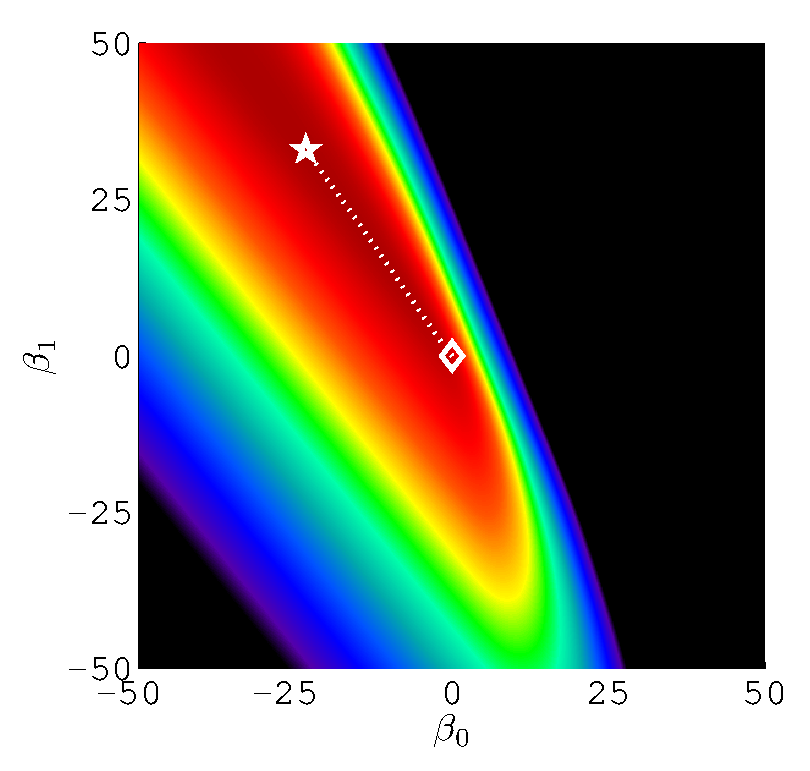
\includegraphics[height=7cm]{objective-surf}
    \caption{$\J(\bb)$ surface}%
    \label{fig:obj-surf}
  \end{subfigure}
  \begin{subfigure}{\plotwidth}
    \centering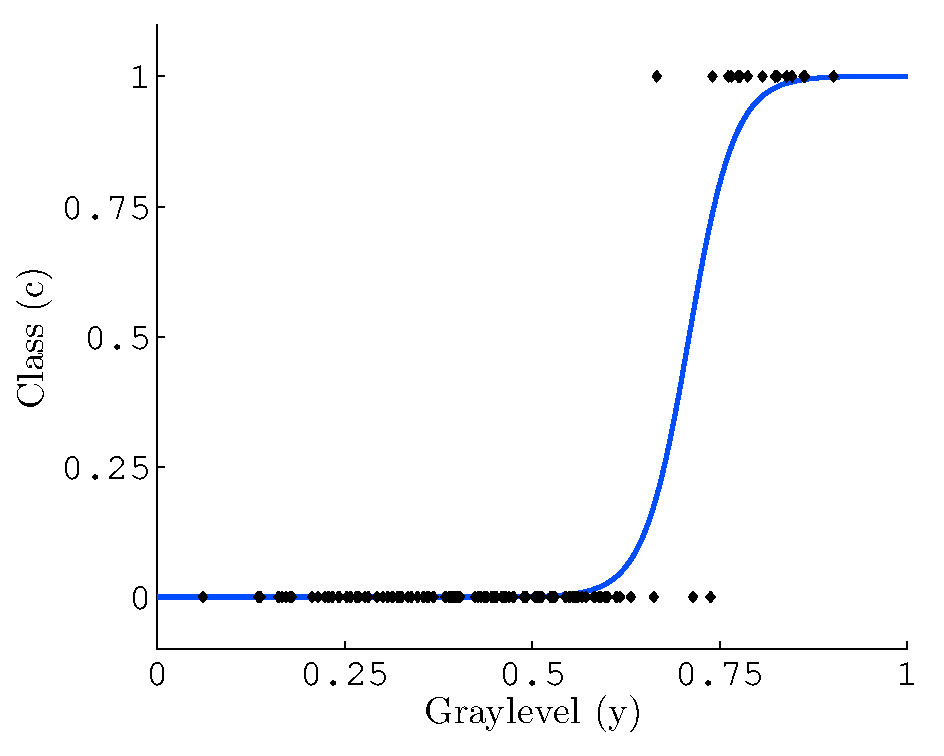
\includegraphics[height=7cm]{objective-LR}
    \caption{Optimal model}%
    \label{fig:obj-lr}
  \end{subfigure}
  \caption{MAP objective function in 2D\@;
    initialization (diamond), fitting (dotted), optimum (star).}
\end{figure}

%%%%%%%%%%%%%%%%%%%%%%%%%%%%%%%%%%%%%%%%%%%%%%%%%%%%%%%%%%%%%%%%%%%%%%%%%%%%%%%%%%%%%%%%%%%%%%%%%%%%
\section{Full Model}
% ==================================================================================================
\subsection{Convergence}
The rate of convergence in each voxel will be unique.
During parallel fitting, it is prudent to stop training after a reasonable number of iterations,
rather than wait for all voxels to achieve a certain stopping criterion,
in case a few aberrant voxels do not converge.
In order to determine this number, the model was fitted using [X] selection(s) of the training data,
and the value of the MAP objective 
%__JK__ not sure how to chose this: see which are faster / slower?


% ==================================================================================================
\subsection{Parameter Images}\label{ss:paramimg}

For comparison with the LPA algorithm, the
\begin{figure}
  \centering
  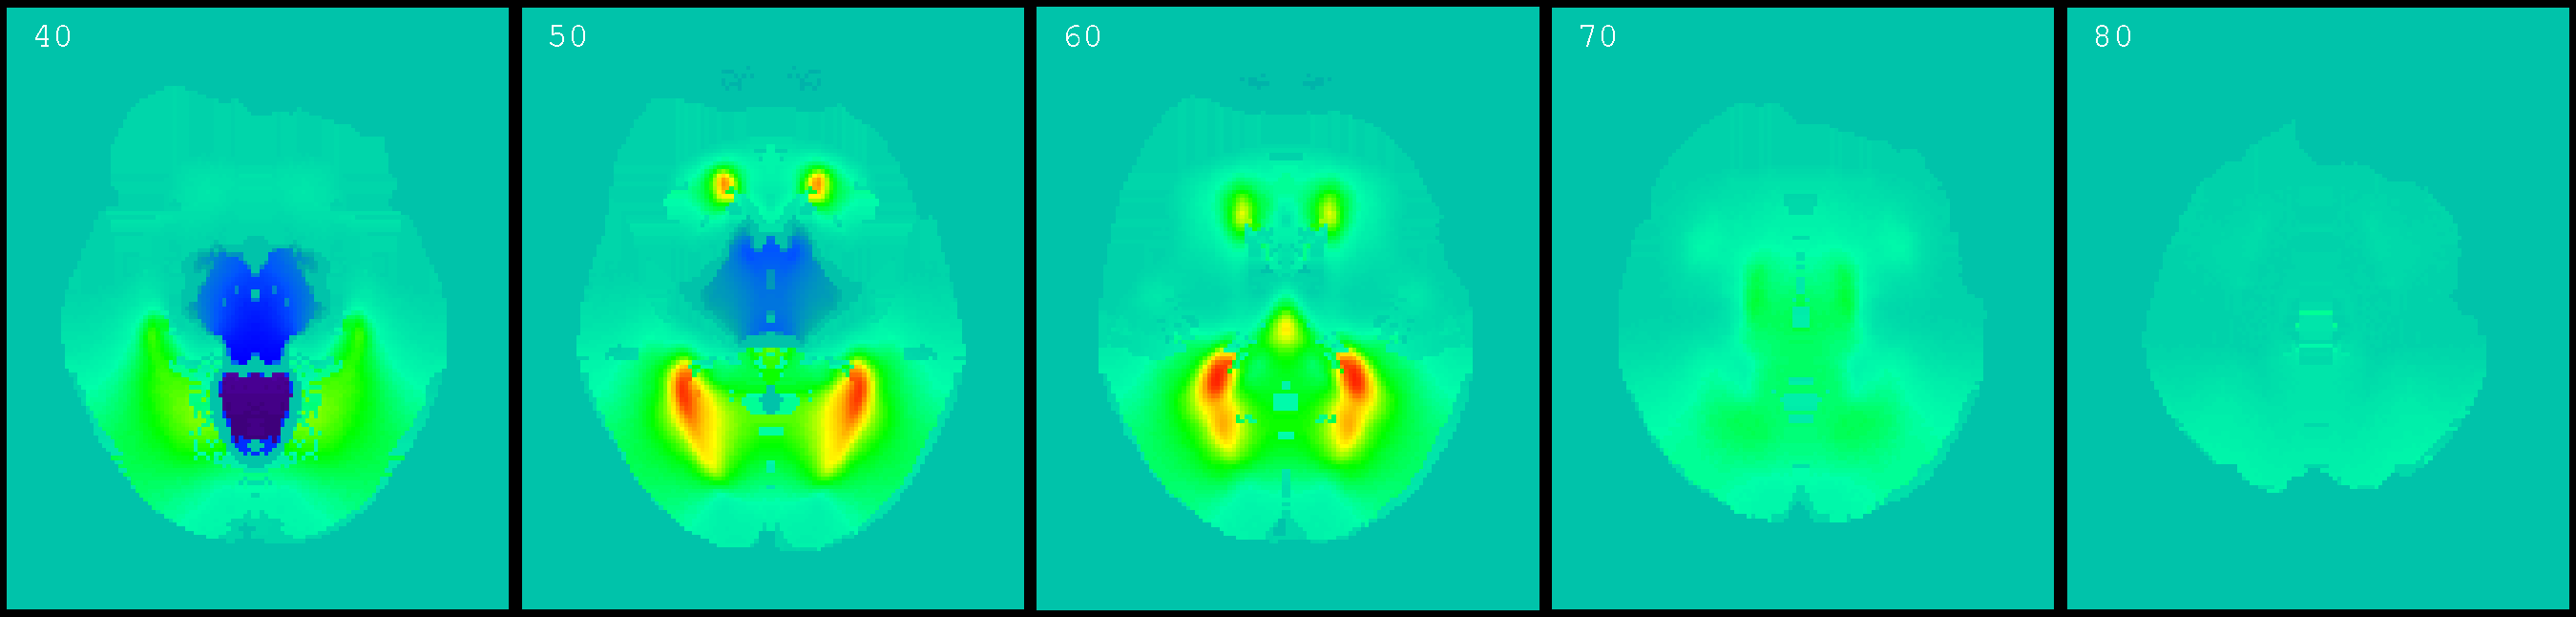
\includegraphics[height=\sliceheight]{beta-LPA.png}
  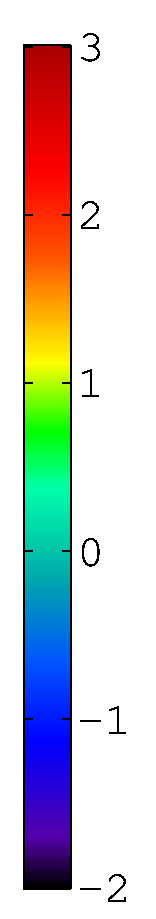
\includegraphics[height=\sliceheight]{cbar-NIH3-LPA}
  \caption{Spatial effect parameter image from the LPA toolbox after registration to MNI space.}%
  \label{fig:B-lpa}
\end{figure}

% ==================================================================================================
\subsection{Quantitative Performance}
% --------------------------------------------------------------------------------------------------
\subsubsection{Regularization}
% ==================================================================================================
\subsection{Comparison with Another Method}
%%%%%%%%%%%%%%%%%%%%%%%%%%%%%%%%%%%%%%%%%%%%%%%%%%%%%%%%%%%%%%%%%%%%%%%%%%%%%%%%%%%%%%%%%%%%%%%%%%%%
\section{Discussion}
%To discuss:
%\begin{itemize}
%  \item central tendency in lesion load: due to histogram equalization. Solution: iteration
%\end{itemize}
% --------------------------------------------------------------------------------------------------
% ==================================================================================================
%%%%%%%%%%%%%%%%%%%%%%%%%%%%%%%%%%%%%%%%%%%%%%%%%%%%%%%%%%%%%%%%%%%%%%%%%%%%%%%%%%%%%%%%%%%%%%%%%%%%

%Finally,  ... (cf. Training / Validation / Test Sets in~\cite{Ripley1995})
  %%%%%%%%%%%%%%%%%%%%%%%%%%%%%%%%%%%%%%%%%%%%%%%%%%%%%%%%%%%%%%%%%%%%%%%%%%%%%%%%%%%%%%%%%%%%%%%%%%%%
% ==================================================================================================
% --------------------------------------------------------------------------------------------------
\chapter{Conclusion}
%%%%%%%%%%%%%%%%%%%%%%%%%%%%%%%%%%%%%%%%%%%%%%%%%%%%%%%%%%%%%%%%%%%%%%%%%%%%%%%%%%%%%%%%%%%%%%%%%%%%
\section{Summary}
%%%%%%%%%%%%%%%%%%%%%%%%%%%%%%%%%%%%%%%%%%%%%%%%%%%%%%%%%%%%%%%%%%%%%%%%%%%%%%%%%%%%%%%%%%%%%%%%%%%%
\section{Future Work}
%Use SPM segment with the FLAIR + T1 to obtain nice GM/WM segmentation. This allows:
%- mixture-model-based standardization of graylevels, since now more accurate?
%- estimated GM to clean up false positives
%
%deep learning advantages:
%- context-aware
%- minimal graylevel standardization necessary
% 
%Graylevel standardization still the key to victory, I think -- need justification of this
%improved registration may also be helpful, since \cite{Klein2009} note that SPM is not the best (time constraints)
% ==================================================================================================
\subsection{Other Features}
% ==================================================================================================
\subsection{Supervised Graylevel Standardization}
% ==================================================================================================
\subsection{Integrative Models}
%There are several advantages to the unified models in the SPM and FSL Segment tools.
%In fact, early ambitions for the current work included integrating
%the WMH segmentation model within SPM Segment.
% advantages:
% - better estimation of bias field
% - more robust registration at low voxel resolution.
% - don't include WMH in estimated healthy tissue classes
% why not:
% - time constraints...
% - prelim investigations: using estimated WM / GM distributions for standardization didn't work.
% ==================================================================================================
\subsection{Open Sourcing}
% --------------------------------------------------------------------------------------------------
% ==================================================================================================
%%%%%%%%%%%%%%%%%%%%%%%%%%%%%%%%%%%%%%%%%%%%%%%%%%%%%%%%%%%%%%%%%%%%%%%%%%%%%%%%%%%%%%%%%%%%%%%%%%%%
	\begin{singlespace}
    \printbibliography%
  \end{singlespace}
  \appendix
  %%%%%%%%%%%%%%%%%%%%%%%%%%%%%%%%%%%%%%%%%%%%%%%%%%%%%%%%%%%%%%%%%%%%%%%%%%%%%%%%%%%%%%%%%%%%%%%%%%%%
% ==================================================================================================
% --------------------------------------------------------------------------------------------------
\chapter{Maths}
This section presents various mathematical results which are not crucial to the thesis.
%%%%%%%%%%%%%%%%%%%%%%%%%%%%%%%%%%%%%%%%%%%%%%%%%%%%%%%%%%%%%%%%%%%%%%%%%%%%%%%%%%%%%%%%%%%%%%%%%%%%
\section{FLAIR MRI Intensity Modelling}\label{s:flairmodel}

%%%%%%%%%%%%%%%%%%%%%%%%%%%%%%%%%%%%%%%%%%%%%%%%%%%%%%%%%%%%%%%%%%%%%%%%%%%%%%%%%%%%%%%%%%%%%%%%%%%%
\section{Histogram Equalization Properties}




% --------------------------------------------------------------------------------------------------
% ==================================================================================================
%%%%%%%%%%%%%%%%%%%%%%%%%%%%%%%%%%%%%%%%%%%%%%%%%%%%%%%%%%%%%%%%%%%%%%%%%%%%%%%%%%%%%%%%%%%%%%%%%%%%

  %%%%%%%%%%%%%%%%%%%%%%%%%%%%%%%%%%%%%%%%%%%%%%%%%%%%%%%%%%%%%%%%%%%%%%%%%%%%%%%%%%%%%%%%%%%%%%%%%%%%
% ==================================================================================================
% --------------------------------------------------------------------------------------------------
\chapter{Implementation}
This appendix contains implementation details.
%%%%%%%%%%%%%%%%%%%%%%%%%%%%%%%%%%%%%%%%%%%%%%%%%%%%%%%%%%%%%%%%%%%%%%%%%%%%%%%%%%%%%%%%%%%%%%%%%%%%
\section{Computing}
All computation in the current work was performed using the following workstation and software:
\begin{itemize}[topsep=0pt,itemsep=-6pt]
  \item \textbf{CPU:} Intel Core i7-6700K 4.00 GHz
  \item \textbf{RAM:} 16.0 GB DDR4
  \item \textbf{GPU:} NVIDIA GeForce GTX 980 Ti
  \item \textbf{OS:} Windows 10 Pro
  \item \textbf{Code:} MATLAB R2011a
\end{itemize}
%%%%%%%%%%%%%%%%%%%%%%%%%%%%%%%%%%%%%%%%%%%%%%%%%%%%%%%%%%%%%%%%%%%%%%%%%%%%%%%%%%%%%%%%%%%%%%%%%%%%
\section{Parallelization}
Speed of model fitting is a significant factor during development,
particularly considering optimization of hyperparameters.
Faster training yields more model iterations, which inevitably bear improvements. 
% ==================================================================================================
\subsection{Model Estimation}\label{s:parallelfit}
While the estimation procedure outlined in \S~\ref{ss:modelfitting}
must be repeated for all standardized voxels in the brain mask,
it is possible to do this in parallel, since every estimation is independent.
To do so, the training data must first be vectorized with respect to spatial location $x$,
and matrix operations expanded explicitly to accommodate the new dimension.
\par
% __JK__ add some details about gpuArray in Matlab?
To begin, the standardized training data from all subjects
-- features $\tilde{\bm{\Y}}_{\gamma}(x)$, with $\tilde{\Y}_{\gamma}^{\et0}=1$,
and labels $\C_{\gamma}(x)$ --
are sampled from nonzero locations in the brain mask $M(x)$.
These data are stored in two matrices $\vox{Y}$ and $\vox{C}$,
with dimensions $[X,N,K+1]$ and $[X,N,1]$, respectively, where
$X$ is the total number of nonzero voxels in the brain mask,
$N$ is the number of subjects, and
$K$ is the number of features.
A similar matrix is constructed for the initial parameters $\bb^{(0)}(x)$, denoted $\vox{B}^{(0)}$,
with dimensions $[X,1,K+1]$.
Let $\vox{Y}_n^k$ denote the vector of data
from all voxels for the $k$\ss{th} feature from the $n$\ss{th} subject,
and so on for $\vox{C}$ and $\vox{B}$.
\par
In order to simplify subsequent calculations,
the feature data are rectified according to the class labels,
before the first iteration, as in
\begin{equation}
  \vox{Y}_n^k =
  \begin{cases}
    +\vox{Y}_n^k, & \vox{C}_n \ge 0.5\\
    -\vox{Y}_n^k, & \vox{C}_n  <  0.5\\
  \end{cases},\qquad\forall\et k \in \{1,\dots,K\}.
\end{equation}
Next, for a given iteration $t$,the following vector-compatible expansions of Equations
(\ref{eq:llgradient}), (\ref{eq:llhessian}), and (\ref{eq:newtonmap})
yield the desired update matrix $\Delta\vox{B}^{(t)}$.
These calculations are performed in \nameref{m:logreg.m}.
Regarding notation:
1.\ the iteration index ${}^{(t)}$ is omitted for clarity,
2.\ element-wise multiplication is denoted by $\circ$, and
3.\ the variable $K$ is now defined as $1$, since this is essential to the simplification.
\par
\begin{align}
  \vox{S} &= \frac{1}{1+e^{+\eta}},\qquad \eta = \vox{B}^0 + \left(\vox{B}^1\ep\vox{Y}^1\right)\\
  \vox{A} &= \vox{S}\ep\left(1-\vox{S}\right)\\
  \vox{G} &= \nabla_{\vox{B}}\L - \lambda\vox{B} \nonumber\\
          &= \left[\begin{array}{c}
               \vox{G}^0 \\
               \vox{G}^1
             \end{array}\right] \nonumber\\
          &= \left[\begin{array}{c}
               \sum_{n=1}^{N}\left( \vox{Y}_n^0\ep\vox{S} \right) \\
               \sum_{n=1}^{N}\left( \vox{Y}_n^1\ep\vox{S} \right)
             \end{array}\right]
           - \lambda\left[\begin{array}{c}
               \vox{B}^0 \\
               \vox{B}^1
             \end{array}\right] \\
  \vox{H} &= \nabla_{\vox{B}}^1\L -\lambda\vox{I} \nonumber\\
          &= \left[\begin{array}{cc}
               \vox{H}^{0,0} & \vox{H}^{0,1} \\
               \vox{H}^{1,0} & \vox{H}^{1,1}
              \end{array}\right] \nonumber\\
          &= \left[\begin{array}{cc}
               \sum_{n=1}^{N}\left( \vox{A}\ep\vox{Y}_n^0\ep\vox{Y}_n^0 \right) & 
               \sum_{n=1}^{N}\left( \vox{A}\ep\vox{Y}_n^1\ep\vox{Y}_n^0 \right) \\
               \sum_{n=1}^{N}\left( \vox{A}\ep\vox{Y}_n^0\ep\vox{Y}_n^1 \right) & 
               \sum_{n=1}^{N}\left( \vox{A}\ep\vox{Y}_n^1\ep\vox{Y}_n^1 \right)
             \end{array}\right] - \lambda\left[\begin{array}{cc} 1 & \\ & 1\end{array}\right]\\
  \vox{D} &= \det{\vox{H}} \nonumber\\
          &= \left(\vox{H}^{0,0}\ep\vox{H}^{1,1}\right)
           - \left(\vox{H}^{0,1}\ep\vox{H}^{1,0}\right) \\
  \Delta\vox{B} &= -\vox{H}^{-1}\vox{G} \nonumber\\
          &= \dfrac{1}{\vox{D}}
             \left[\begin{array}{cc}
               \left(\vox{H}^{1,1}\ep\vox{G}^{0} - \vox{H}^{1,0}\ep\vox{G}^{1} \right) & 
               \left(\vox{H}^{0,1}\ep\vox{G}^{1} - \vox{H}^{0,0}\ep\vox{G}^{0} \right)
             \end{array}\right]^{T}
\end{align}
% ==================================================================================================
\subsection{Image Deformations}
% __JK__ describe the SPM deformations workflow
% Following training, ...
%
% While these deformations are saved after initial estimation,
% their application is computationally expensive.
%%%%%%%%%%%%%%%%%%%%%%%%%%%%%%%%%%%%%%%%%%%%%%%%%%%%%%%%%%%%%%%%%%%%%%%%%%%%%%%%%%%%%%%%%%%%%%%%%%%%
\section{Manual Segmentations}
It was necessary to create and edit a small number of binary segmentation masks during this work.
To do this, the Editor module from the 3D Slicer imaging platform~\cite{Fedorov2012} was used,%
\footnote{3D Slicer Editor tool documentation is available here:
  \hreftt{https://www.slicer.org/wiki/Documentation/4.6/Modules/Editor}.}
including the Wand, Paint, and Erase functions.
Figure~\ref{fig:m08-rev-slicer} shows the user interface during a lesion segmentation.
\begin{figure}[h]
  \centering
  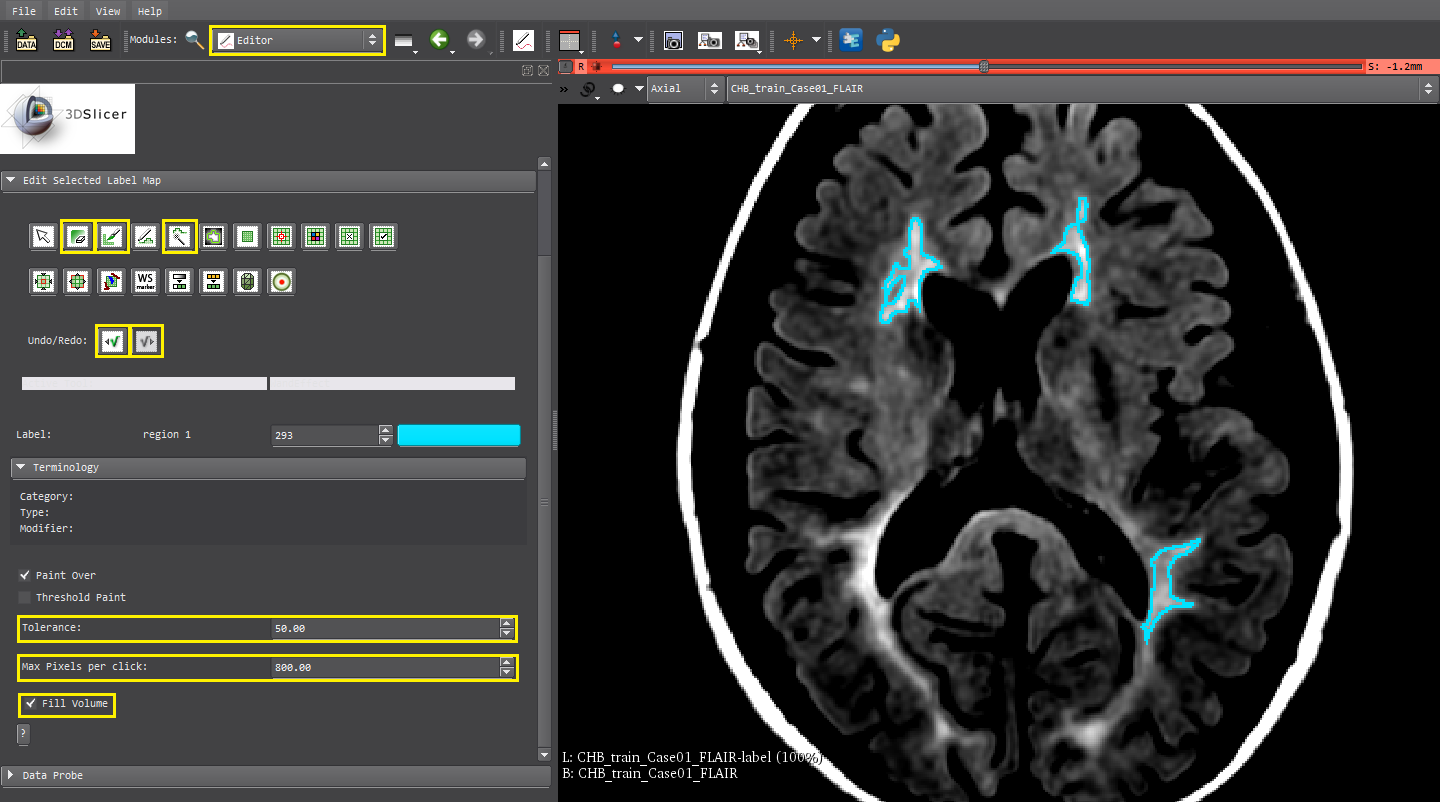
\includegraphics[width=\textwidth]{m08rev-slicer.png}
  \caption{3D Slicer user interface for performing in-house manual segmentations and revisions.
    The tools used are highlighted in yellow, while the in-progress segmentation is shown in blue.}%
  \label{fig:m08-rev-slicer}
\end{figure}
% ==================================================================================================
\subsection{MS 2008 WMH Masks}\label{ss:m08-rev}
Since the reported performance of an automatic segmentation algorithm depends on
the manual segmentations to which it is compared,
it is important to obtain good manual segmentations.
Unfortunately, the original manuals in the MS 2008 Segmentation Challenge
contained obvious artifacts and inconsistencies,
as shown at left in Figure~\ref{fig:m08-rev}.
Therefore, it was deemed necessary to redo these manuals.
The resulting revisions are shown at right in Figure~\ref{fig:m08-rev}.
\begin{figure}
  \centering
  \begin{minipage}{6cm}
    \begin{subfigure}{\textwidth}
      \centering\subcaption{Original}%
      \label{fig:m08-rev-o}
      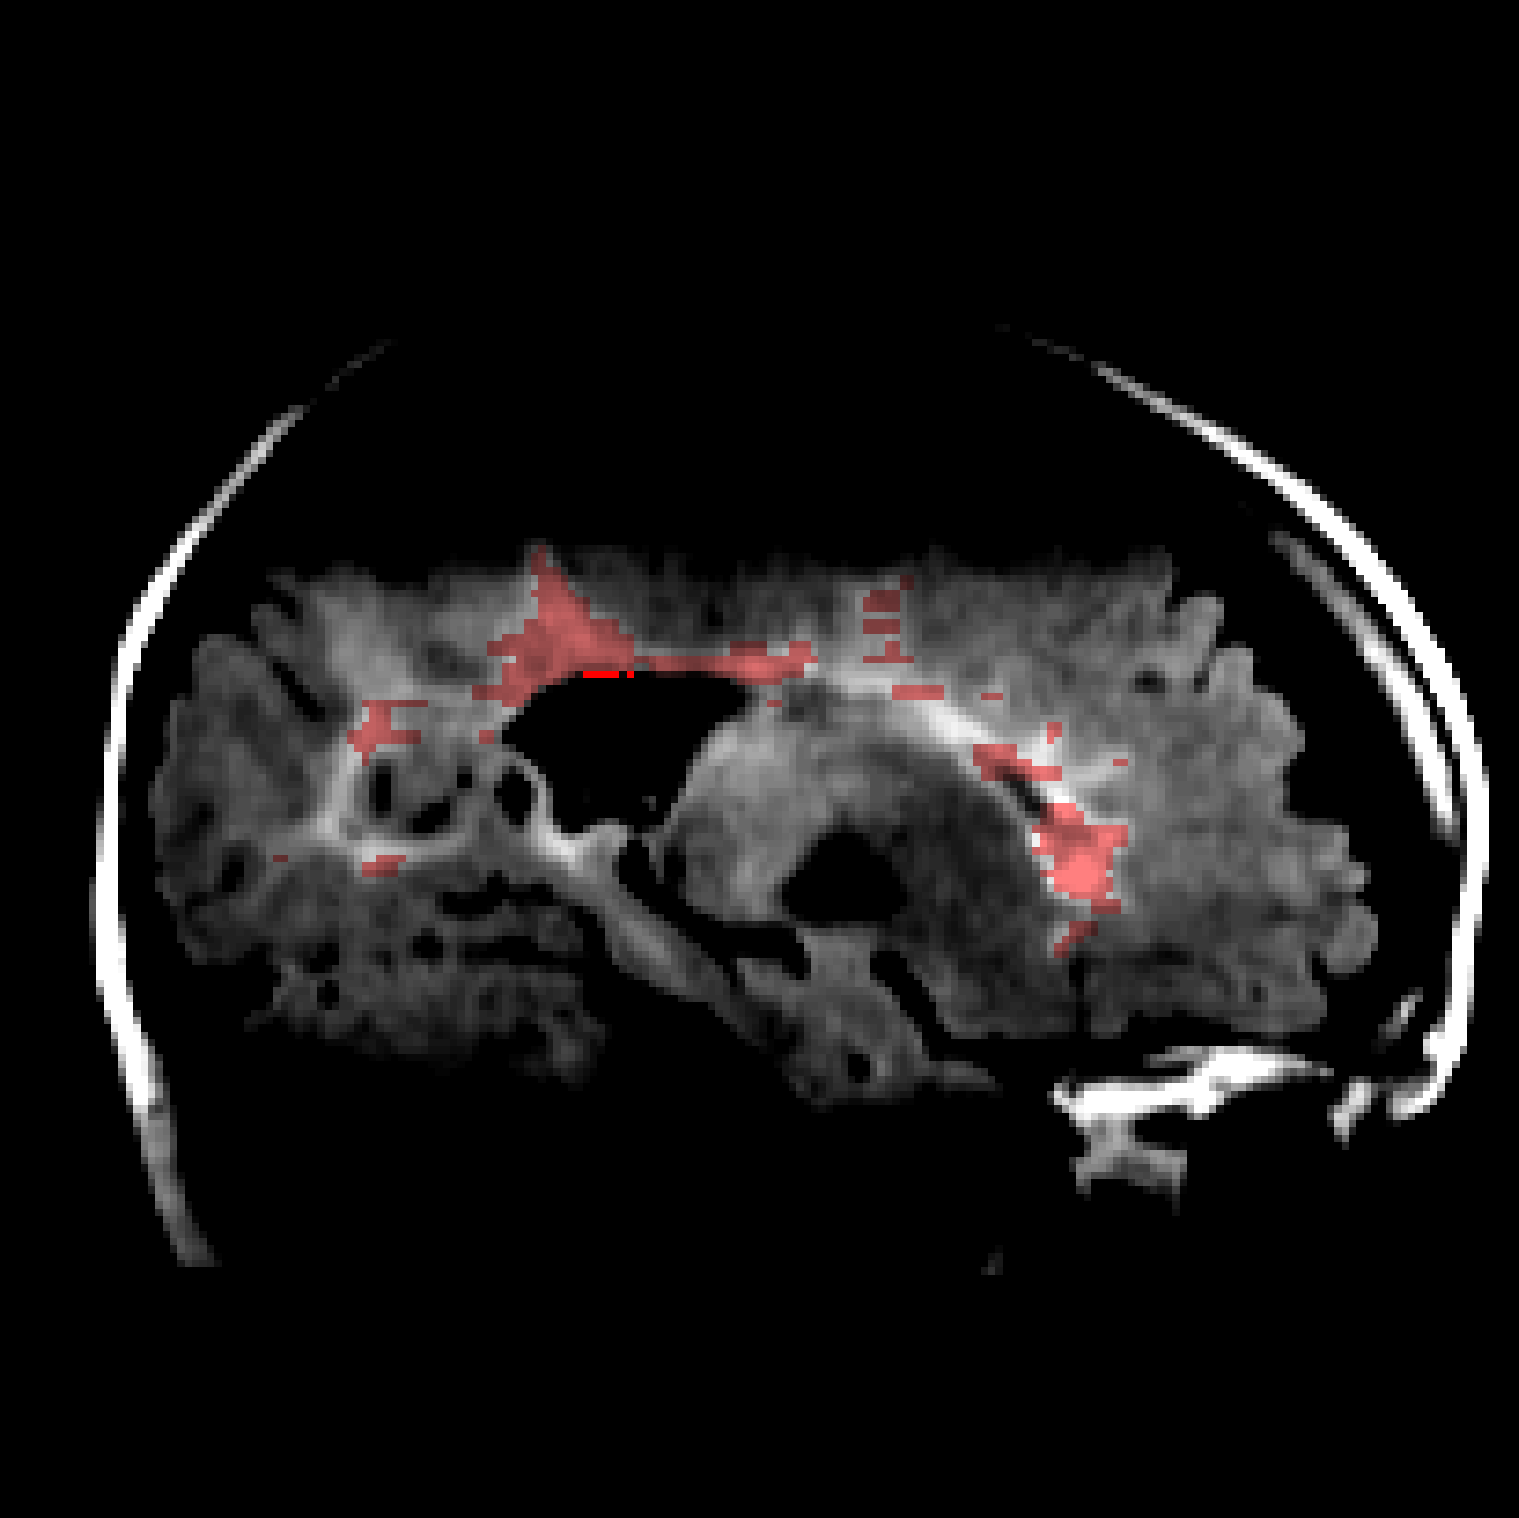
\includegraphics[height=6cm]{m08rev-01-d2-z146-o}\\[0.2em]
      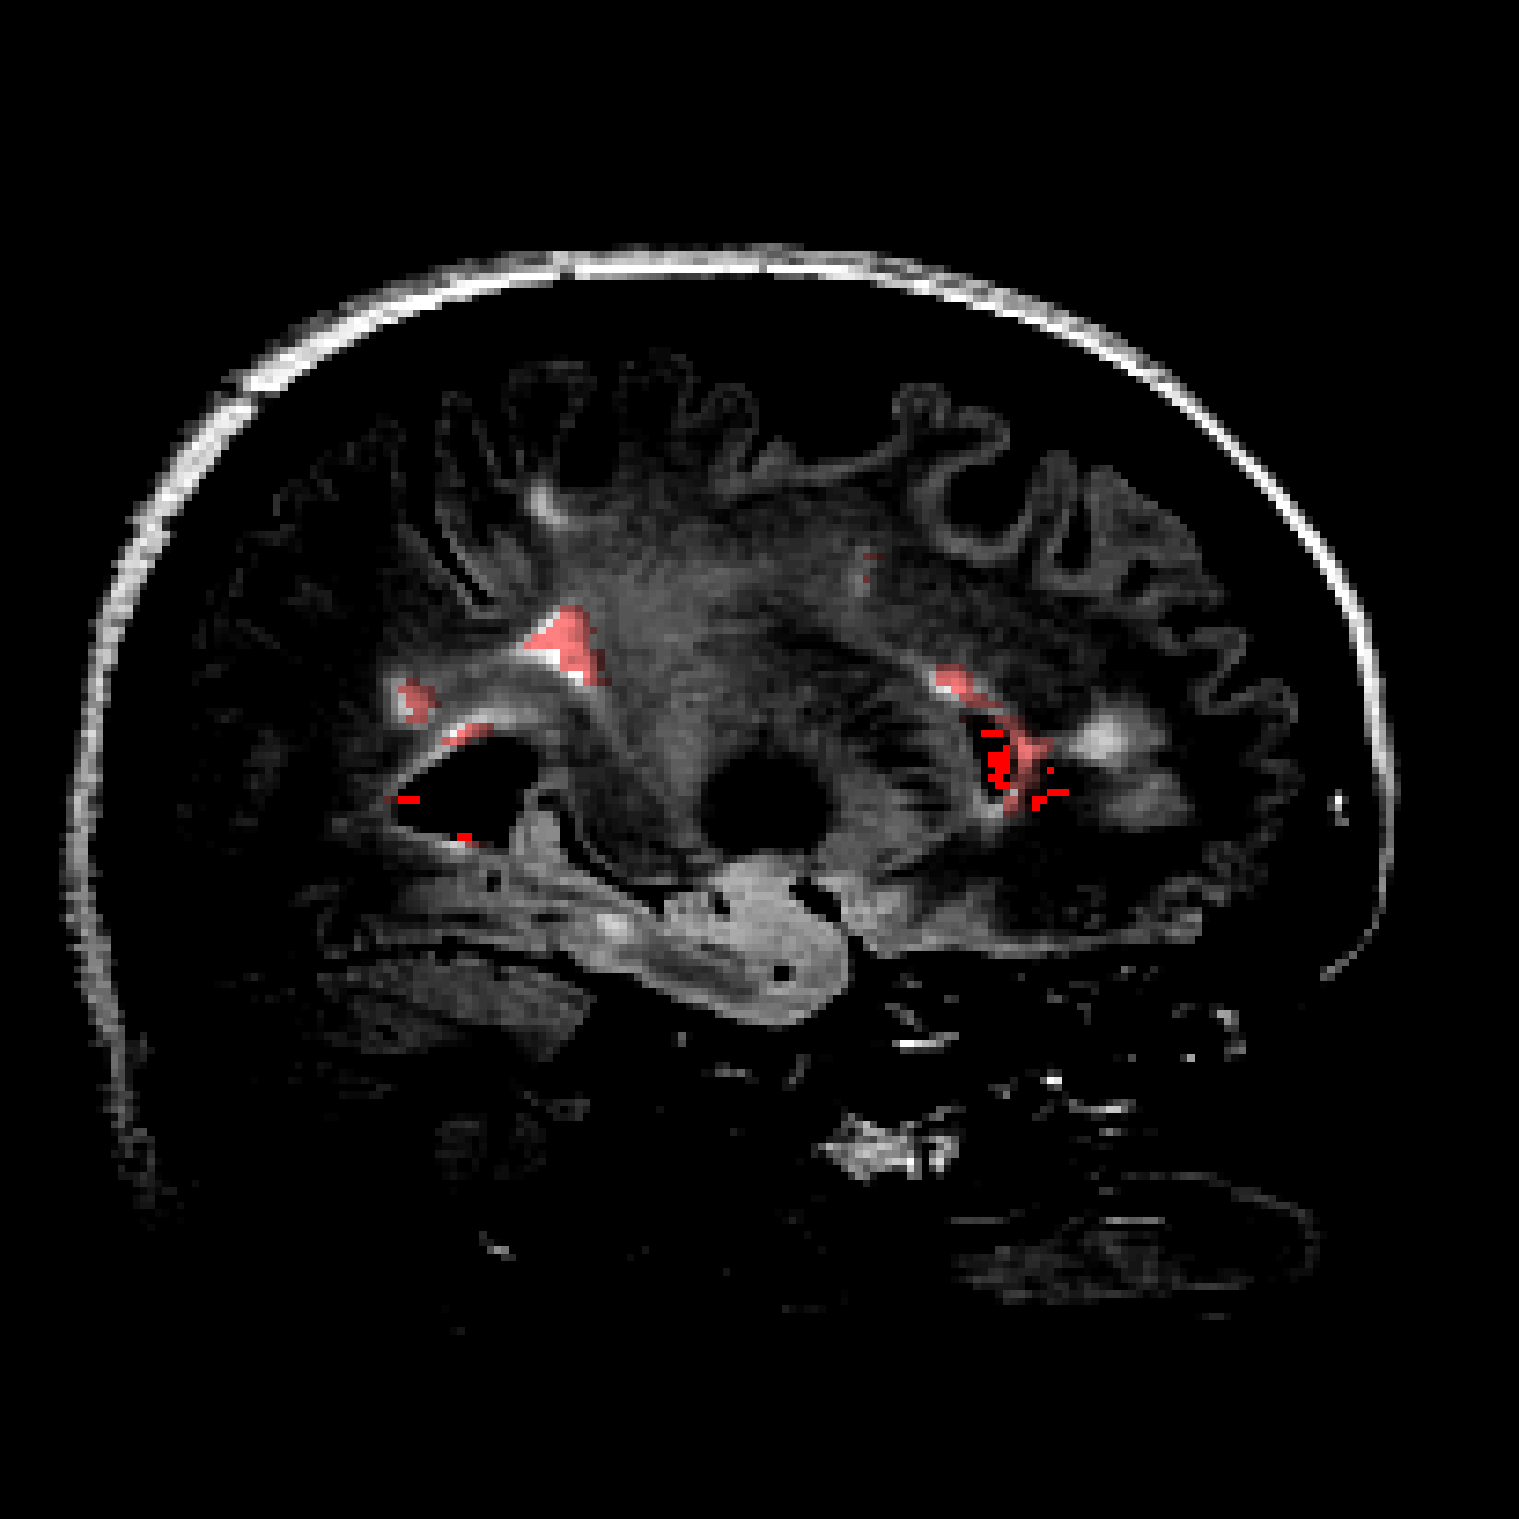
\includegraphics[height=6cm]{m08rev-05-d2-z107-o}\\[0.2em]
      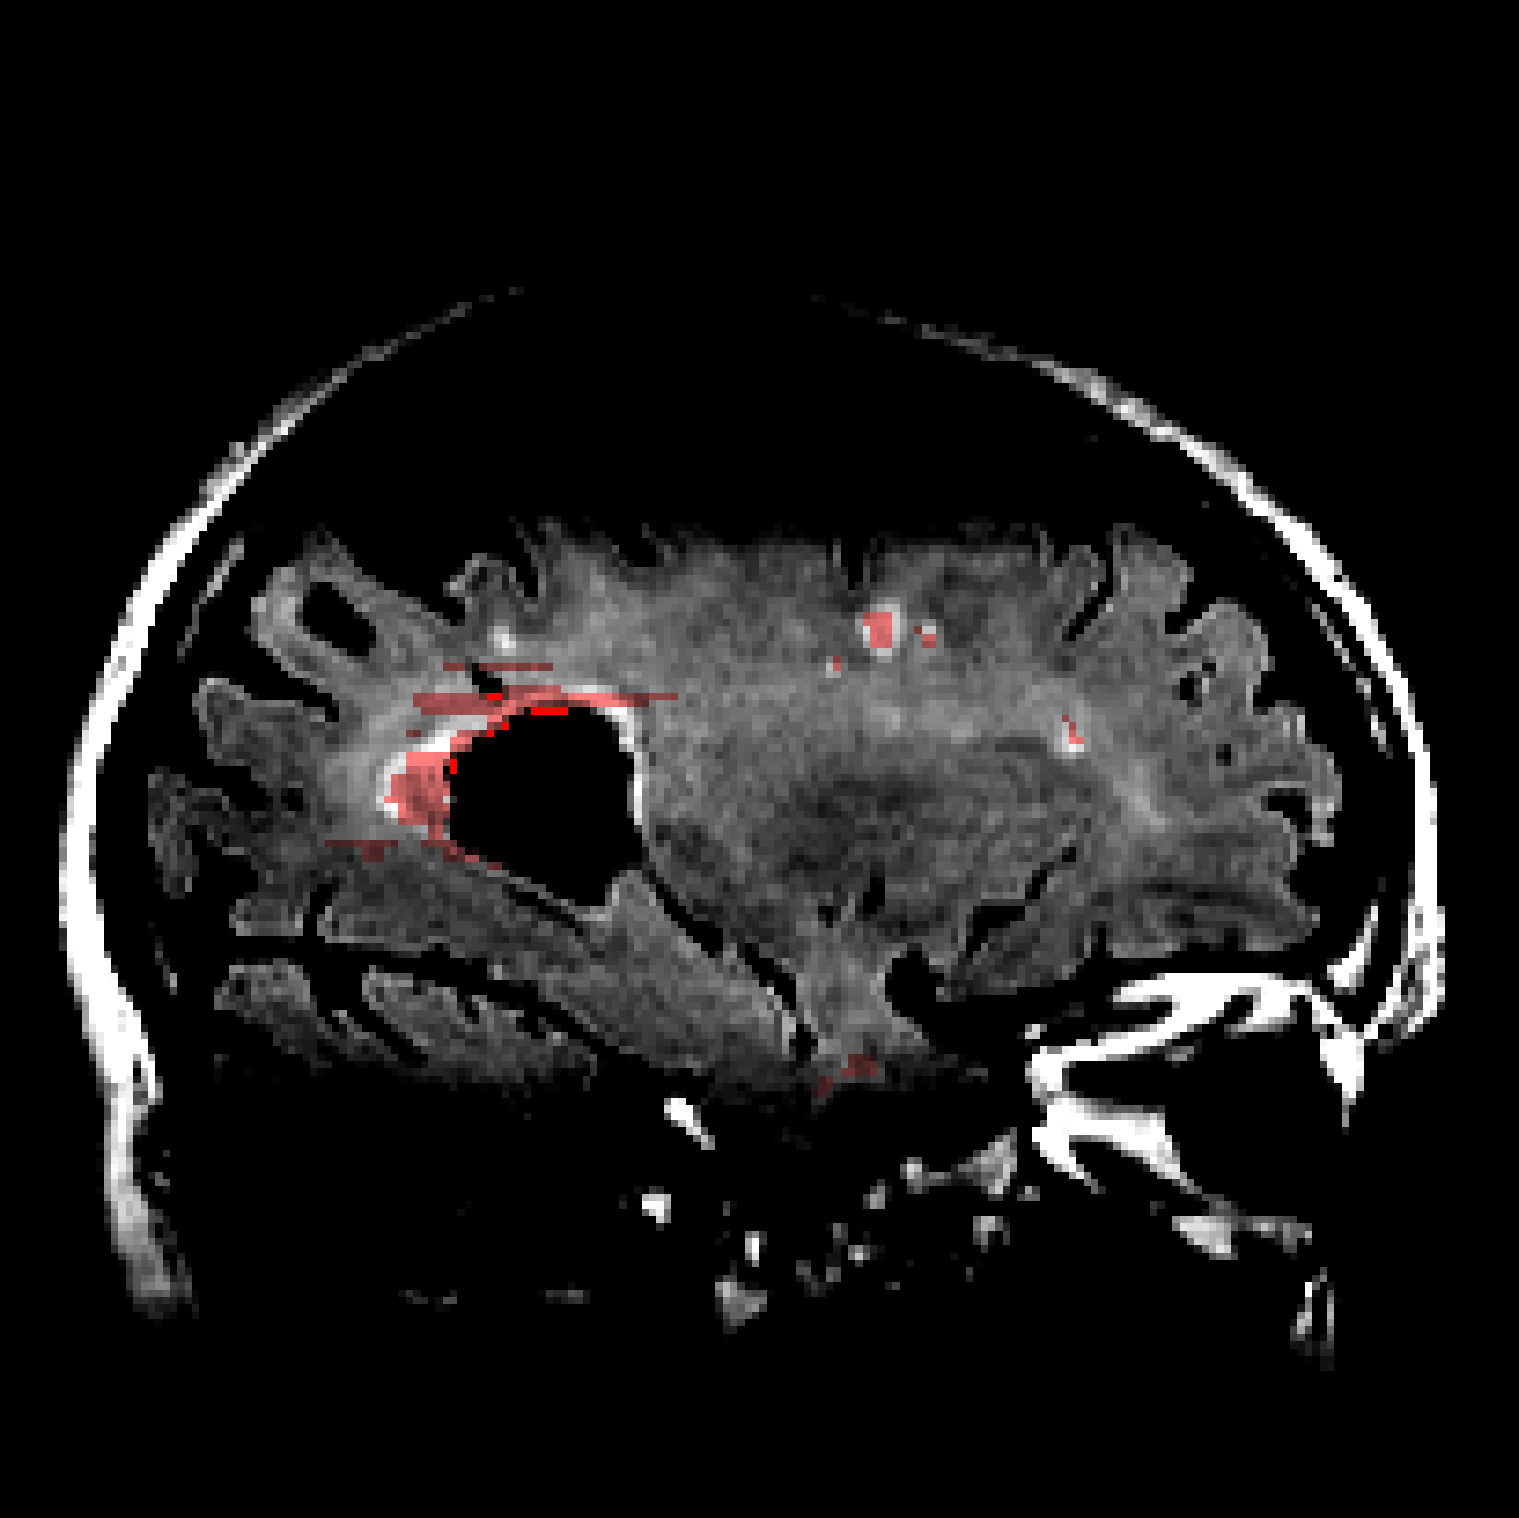
\includegraphics[height=6cm]{m08rev-06-d2-z101-o}
    \end{subfigure}
  \end{minipage}
  \begin{minipage}{6cm}
    \begin{subfigure}{\textwidth}
      \centering\subcaption{Revision}%
      \label{fig:m08-rev-r}
      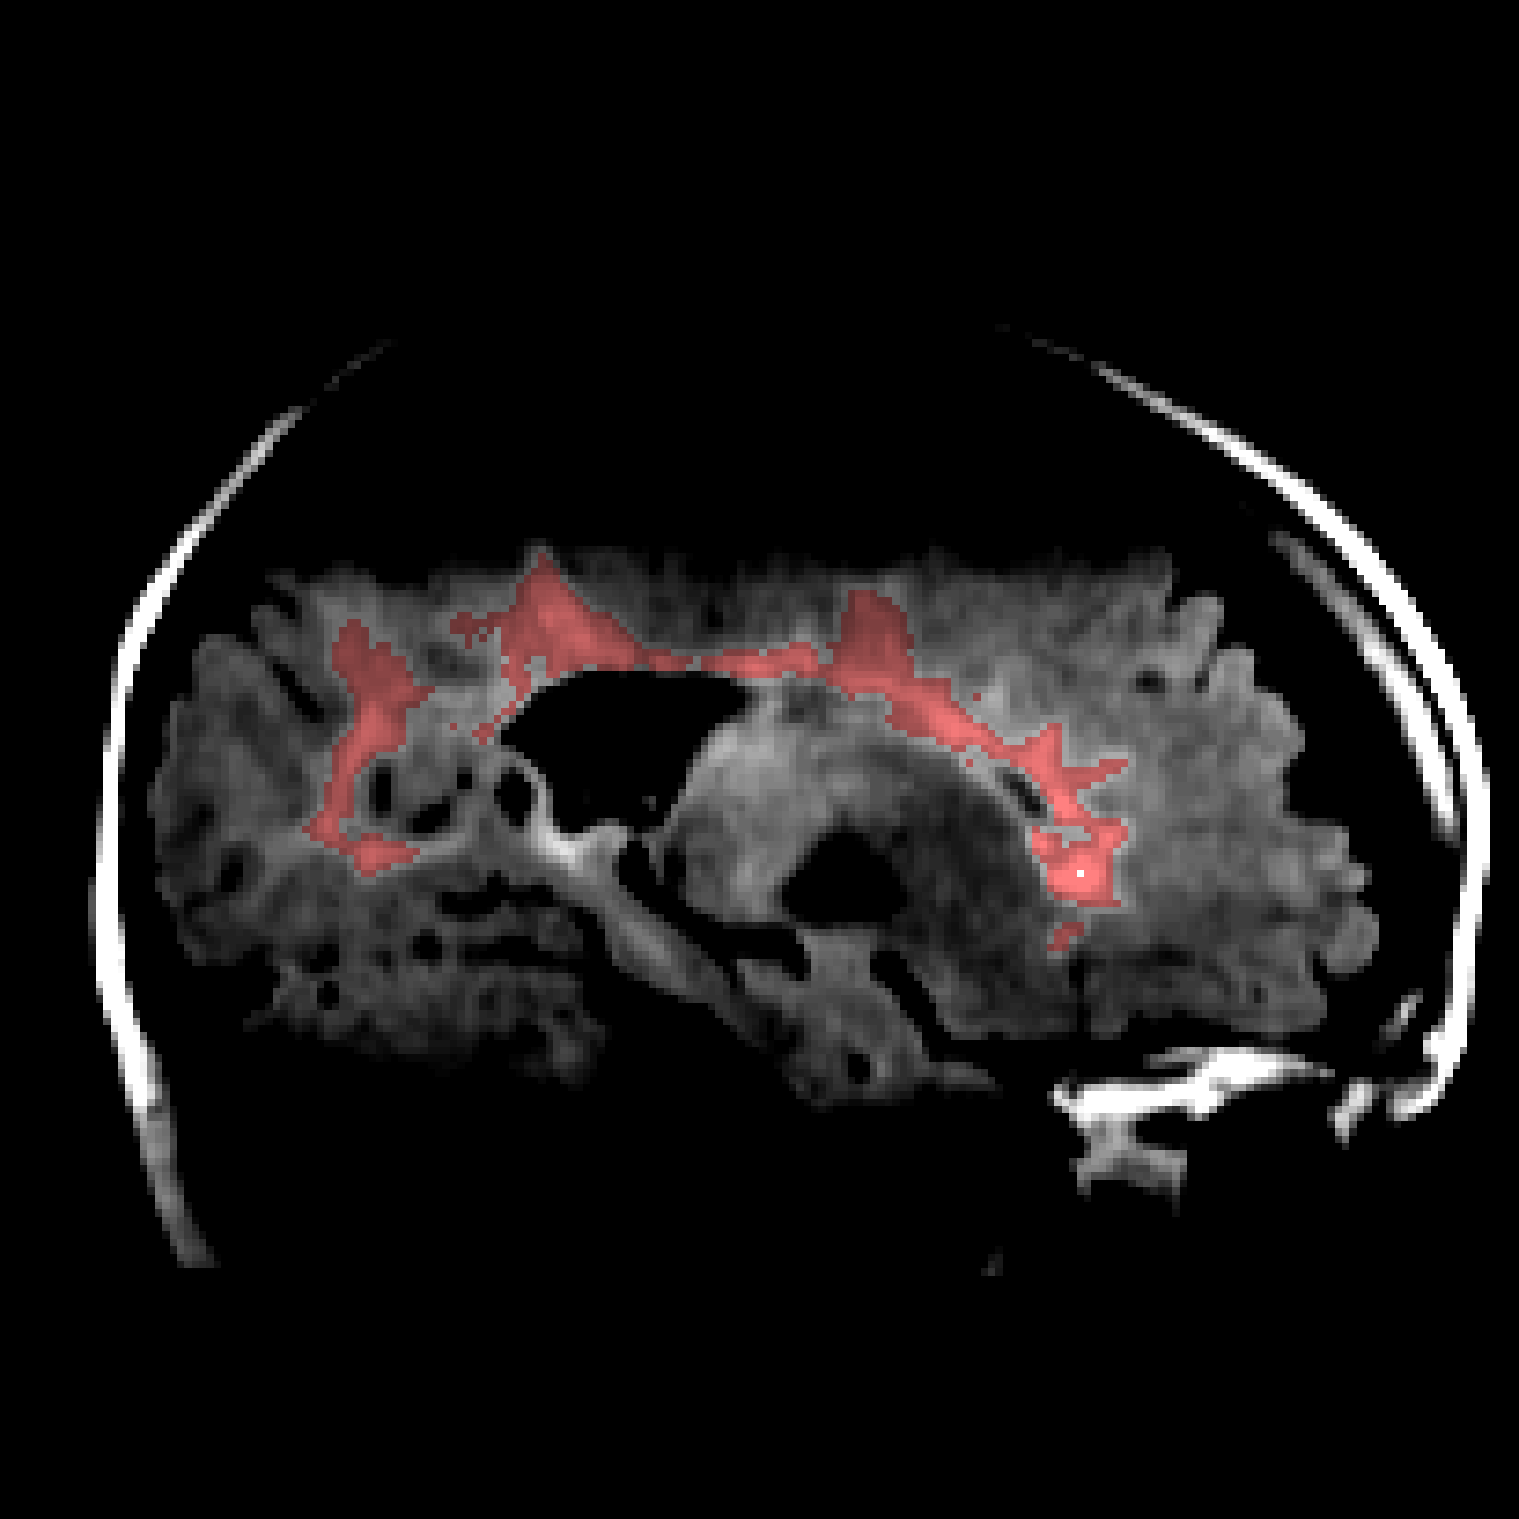
\includegraphics[height=6cm]{m08rev-01-d2-z146-r}
        \makebox[0pt][r]{\textcolor{white}{ CHB 01 }}\\[0.2em]
      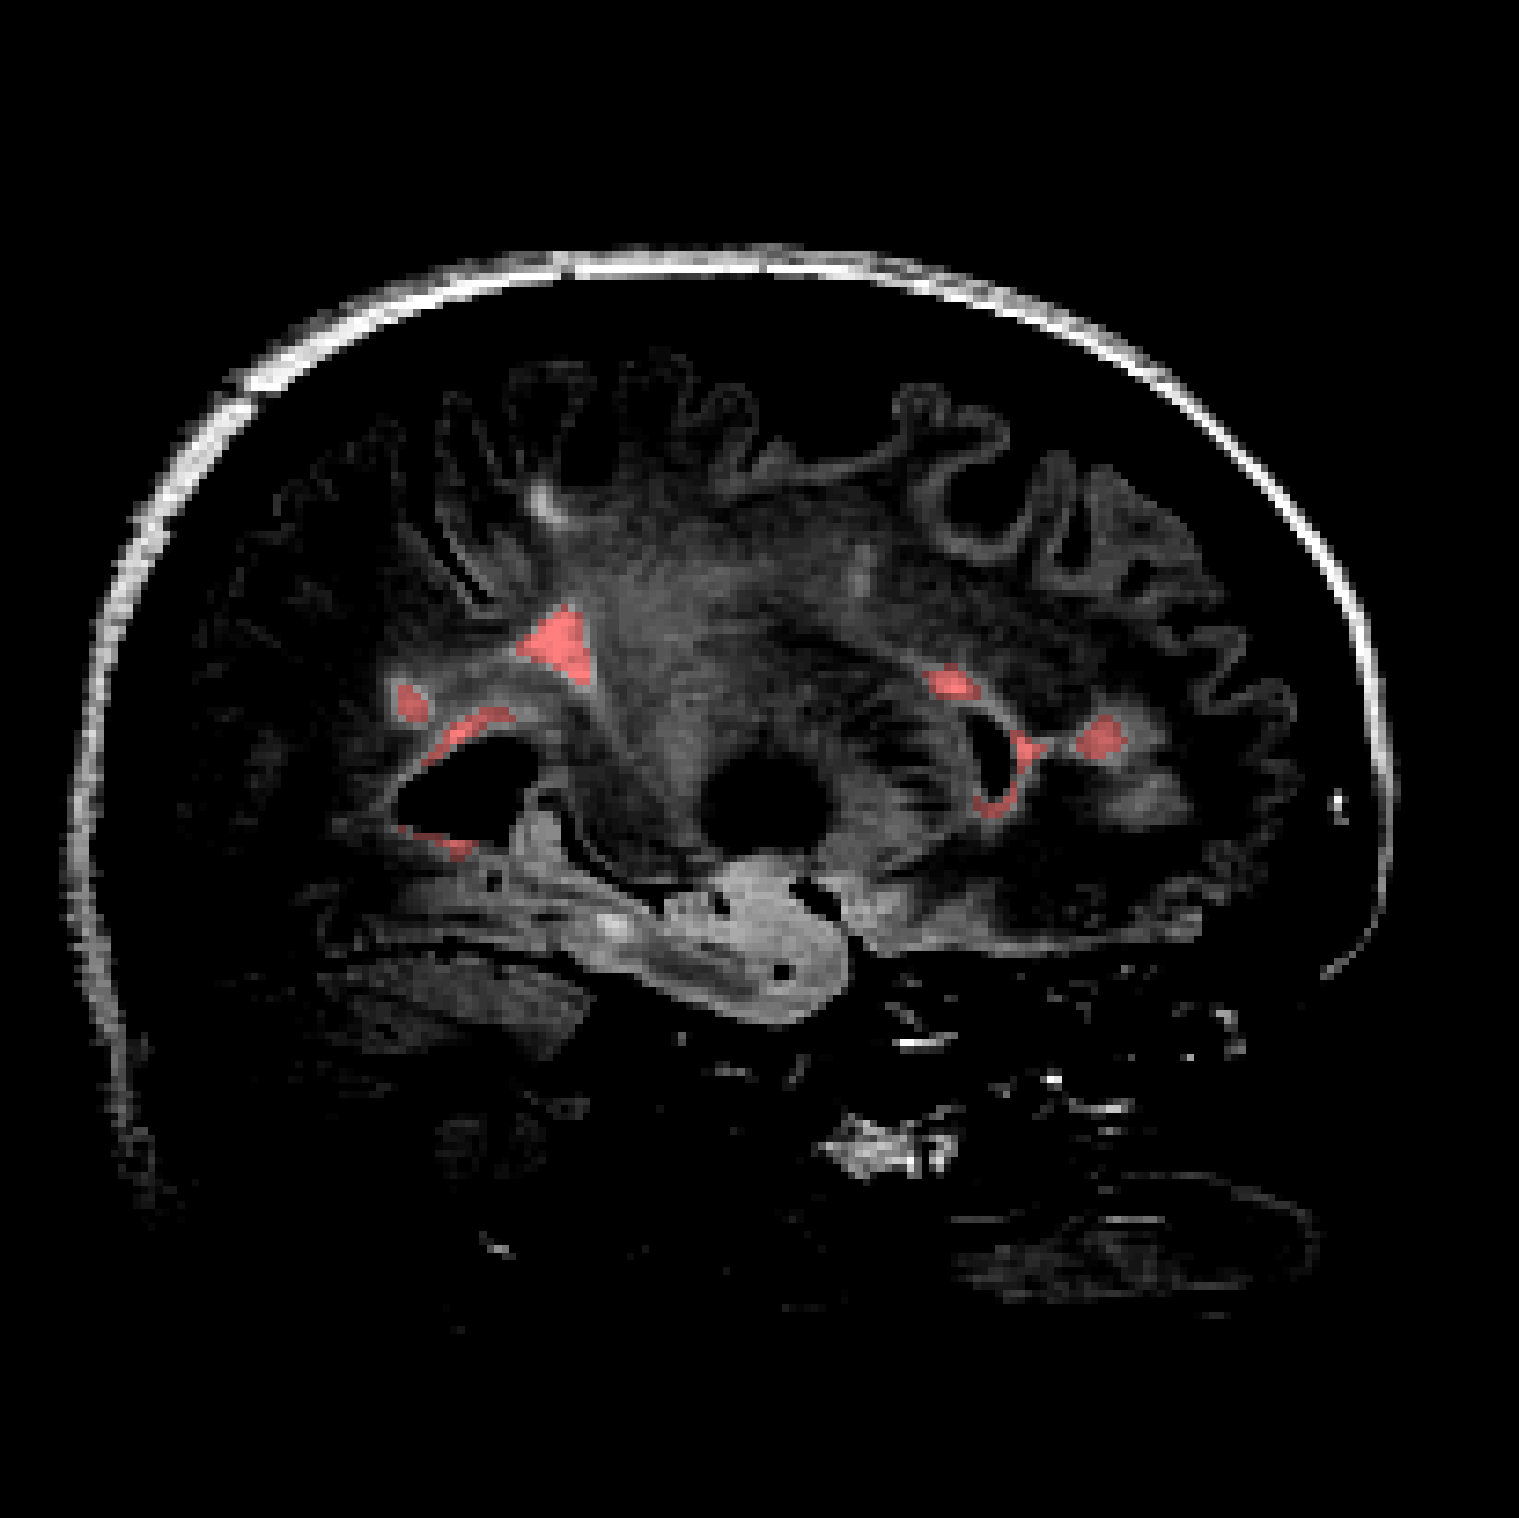
\includegraphics[height=6cm]{m08rev-05-d2-z107-r}
        \makebox[0pt][r]{\textcolor{white}{ CHB 05 }}\\[0.2em]
      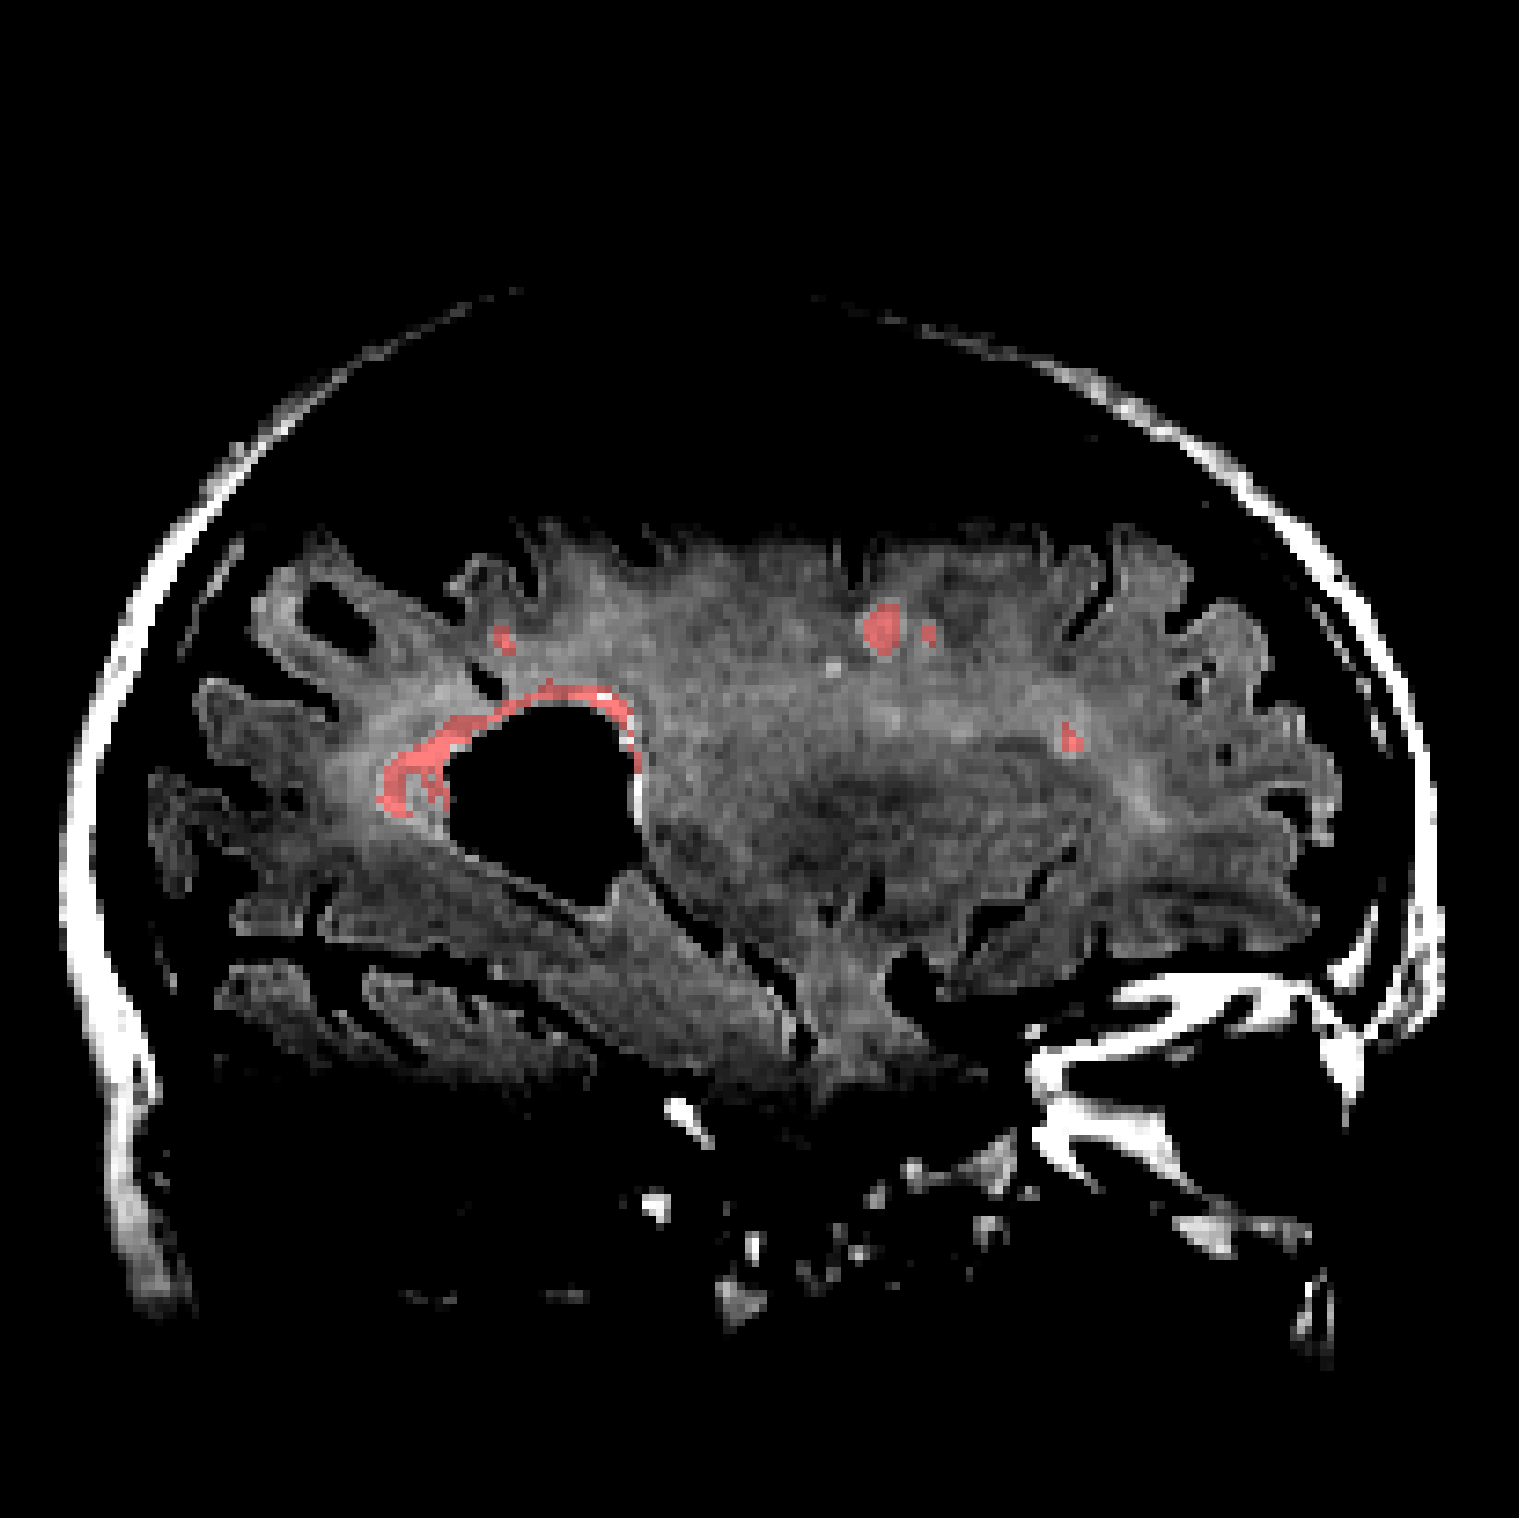
\includegraphics[height=6cm]{m08rev-06-d2-z101-r}
        \makebox[0pt][r]{\textcolor{white}{ CHB 06 }}
    \end{subfigure}
  \end{minipage}
  \caption{Example revisions to the manual segmentations for the MS 2008 challenge dataset.}%
  \label{fig:m08-rev}
\end{figure}
% ==================================================================================================
\subsection{Brain Mask}\label{ss:brainmask}
In order to vectorize image data for parallel processing,
a binary mask selecting voxels of interest in standardized space is also required.
Since only voxels in the brain are of interest, this mask is called a ``brain mask''.
The brain mask used here was derived from
the ICBM tissue prior images~\cite{Mazziotta2001} in MNI space:
after initial thresholding of the combined $\gm{}+\wm{}+\csf{}$ probabilities at 0.5,
manual refinements were completed and symmetry was enforced.
The mask is slightly small on purpose,
since tissues outside the brain are frequently bright in FLAIR images,
and can be mistaken for lesions by naive models.
The resulting mask is shown in Figure~\ref{fig:brainmask}.
\begin{figure}
  \centering
  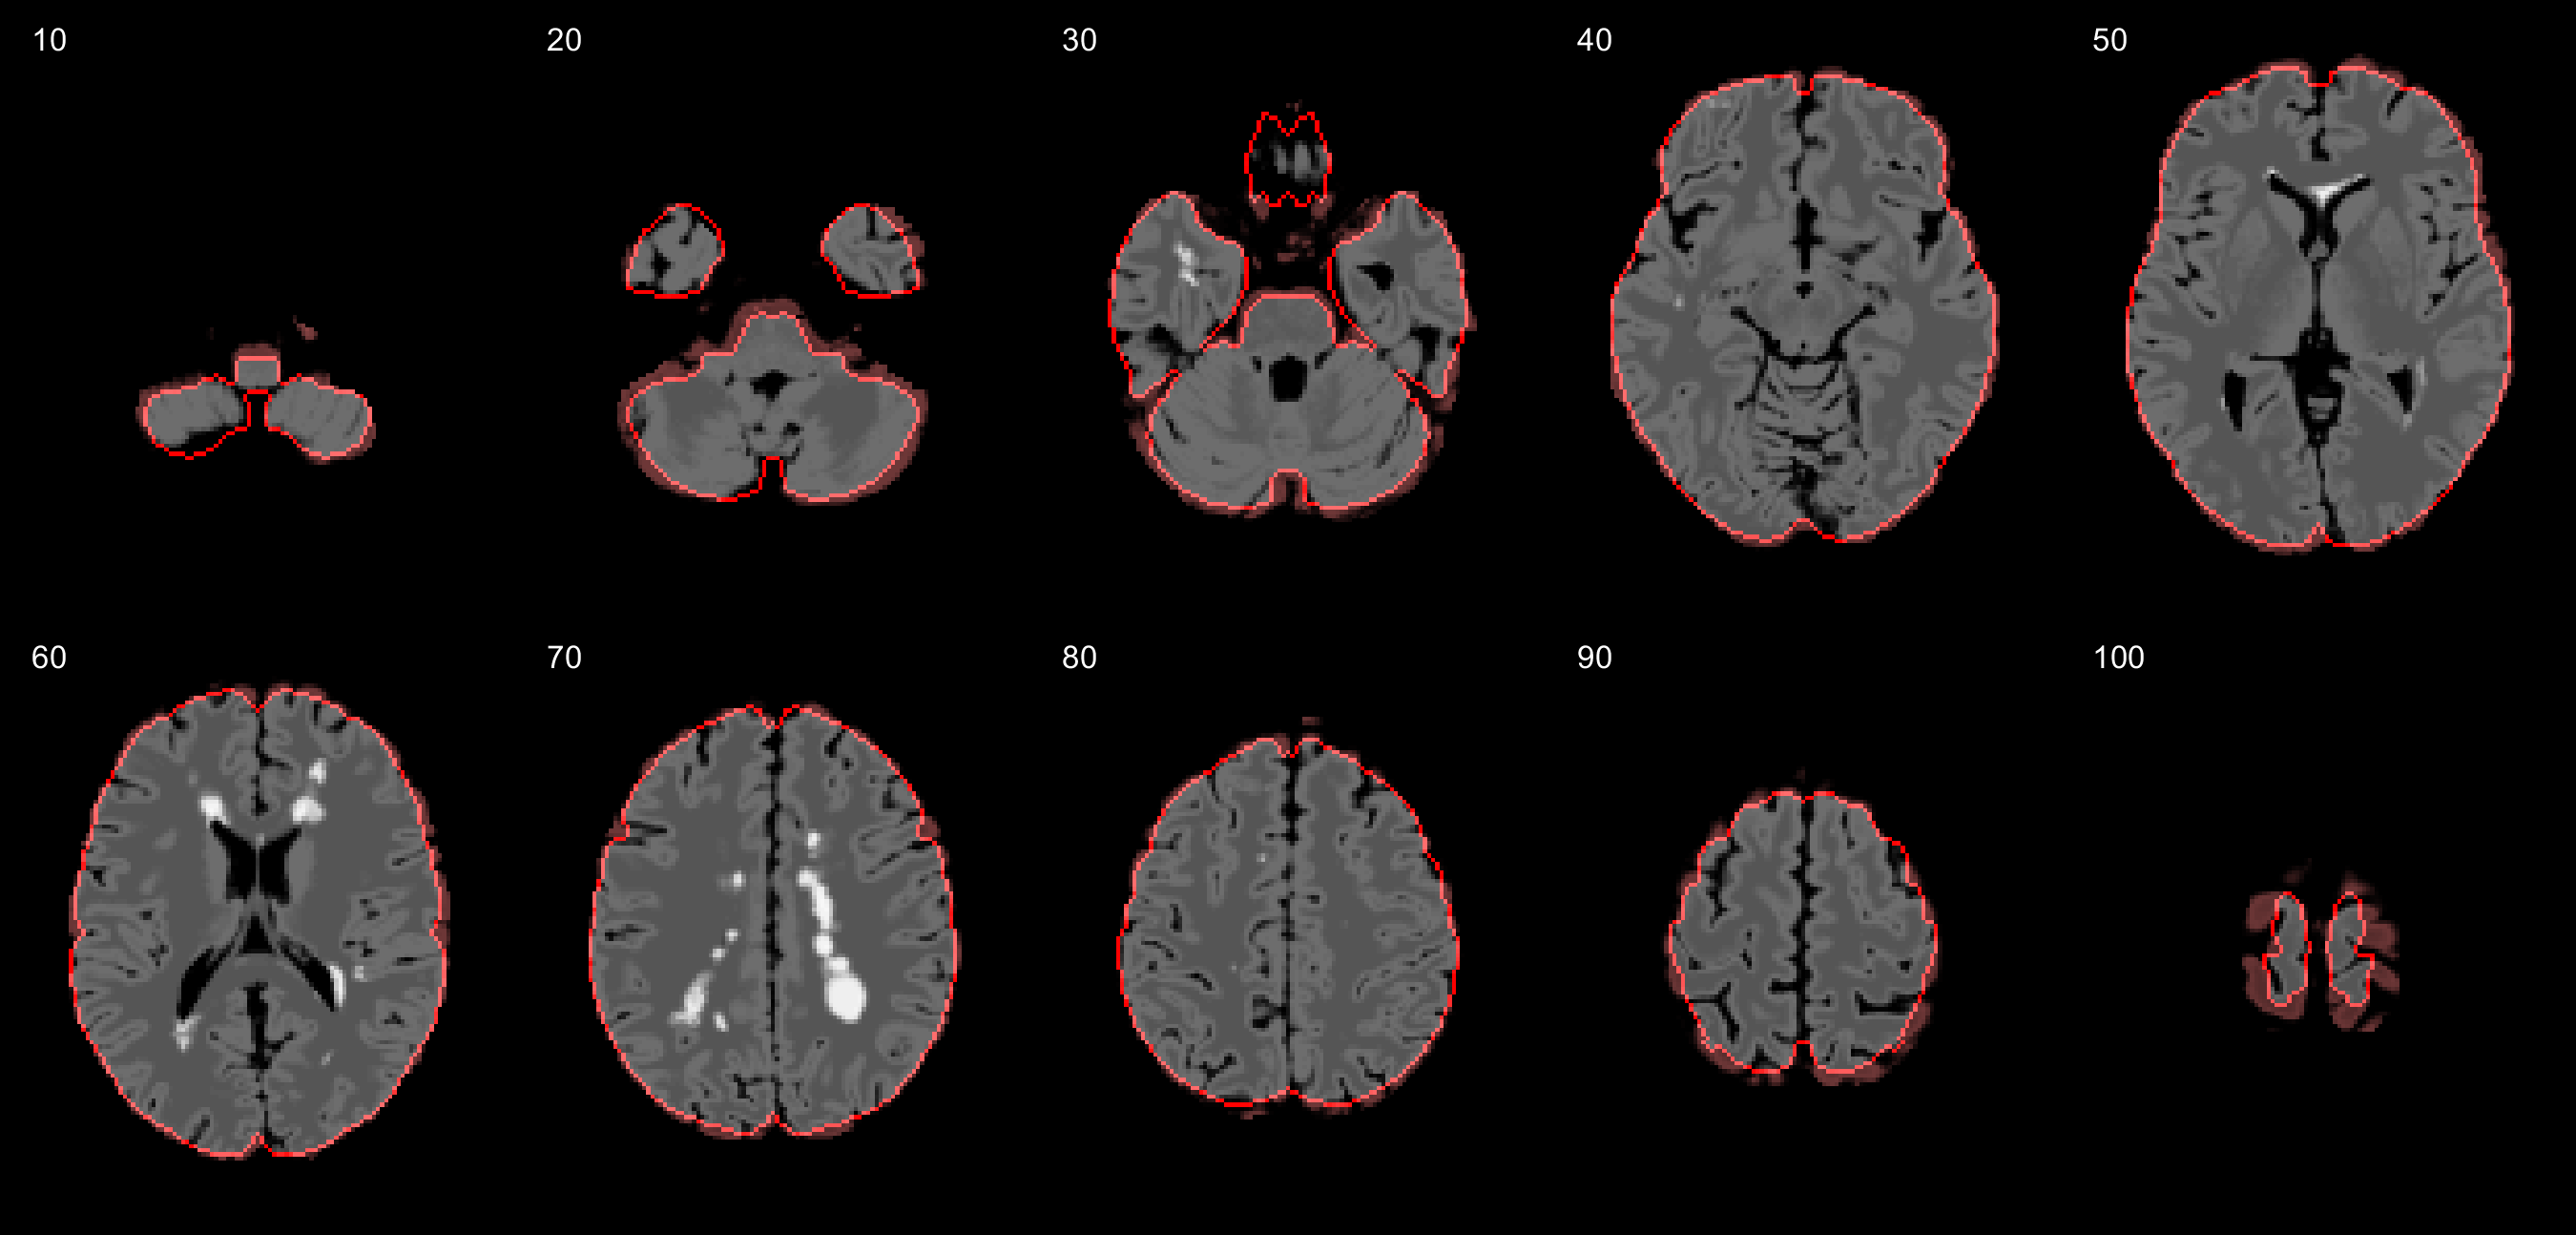
\includegraphics[height=2\sliceheight]{brainmask.png}
  \caption{Manually refined brain mask in MNI space, overlaid on a simulated BrainWeb FLAIR image.
    Mask outline is highlighted in red; inclusions are shown in grayscale; exclusions tinted red.}%
  \label{fig:brainmask}
\end{figure}
% --------------------------------------------------------------------------------------------------
% ==================================================================================================
%%%%%%%%%%%%%%%%%%%%%%%%%%%%%%%%%%%%%%%%%%%%%%%%%%%%%%%%%%%%%%%%%%%%%%%%%%%%%%%%%%%%%%%%%%%%%%%%%%%%

  %%%%%%%%%%%%%%%%%%%%%%%%%%%%%%%%%%%%%%%%%%%%%%%%%%%%%%%%%%%%%%%%%%%%%%%%%%%%%%%%%%%%%%%%%%%%%%%%%%%%
% ==================================================================================================
% --------------------------------------------------------------------------------------------------
\chapter{Code}
\includecode{hypdef.m}
%\includecode{arbiter.m}
%\includecode{logreg.m}
% --------------------------------------------------------------------------------------------------
% ==================================================================================================
%%%%%%%%%%%%%%%%%%%%%%%%%%%%%%%%%%%%%%%%%%%%%%%%%%%%%%%%%%%%%%%%%%%%%%%%%%%%%%%%%%%%%%%%%%%%%%%%%%%%

  %%%%%%%%%%%%%%%%%%%%%%%%%%%%%%%%%%%%%%%%%%%%%%%%%%%%%%%%%%%%%%%%%%%%%%%%%%%%%%%%%%%%%%%%%%%%%%%%%%%%%
% ==================================================================================================
% --------------------------------------------------------------------------------------------------
\chapter{Resources}
Here are some helpful links for WMH segmentation research.
\section{Toolboxes}

\section{Neuroimaging Toolboxes}

\section{WMH Segmentation Toolboxes}
LST: Lesion Segmentation Tool~\cite{Schmidt2012,Schmidt2015} for SPM
-- \hreftt{http://www.statistical-modelling.de/lst.html}

\section{Prior Work}
\subsection{Competitions \& Open Access Data}
\begin{tabu} to \textwidth {llcl}
	\toprule
	Name                & Conference  &        Ref.         & Link                                                     \\ \midrule
	MS LSC              & MICCAI 2008 & ~\cite{MSSEG2008}~  & \hreftt{http://www.ia.unc.edu/MSseg/}                    \\
	Longitudinal MS LSC & ISBI 2015   & ~\cite{MSISBI2015}~ & \hreftt{http://iacl.ece.jhu.edu/index.php/MSChallenge}   \\
	MS LSC              & MICCAI 2016 & ~\cite{MSSEG2016}~  & \hreftt{https://portal.fli-iam.irisa.fr/msseg-challenge} \\
	WMH LSC             & MICCAI 2017 & ~\cite{WMHSEG2017}~ & \hreftt{http://wmh.isi.uu.nl/}                           \\ \bottomrule
\end{tabu}\\
``LSC'' -- Lesion Segmentation Challenge
\subsection{Prior Work Table}
\hreftt{www.uoguelph.ca/~jknigh04/wmlseg/table.html}

% --------------------------------------------------------------------------------------------------
% ==================================================================================================
%%%%%%%%%%%%%%%%%%%%%%%%%%%%%%%%%%%%%%%%%%%%%%%%%%%%%%%%%%%%%%%%%%%%%%%%%%%%%%%%%%%%%%%%%%%%%%%%%%%%

\end{document}
%%%%%%%%%%%%%%%%%%%%%%%%%%%%%%%%%%%%%%%%%%%%%%%%%%%%%%%%%%%%%%%%%%%%%%%%%%%%%%%%%%%%%%%%%%%%%%%%%%%%
